\documentclass[
	noindent
]{elteikthesis}[2024/04/26]

\title{Fotográfiai témafelismerés neurális hálózatokkal nagy adathalmazon.} 
\date{2025}

% Author's metadata
\author{Sándor Balázs}
\degree{Programtervező informatikus MSc}

% Superivsor(s)' metadata
\supervisor{Dr. Kiss Attila Elemér}
\affiliation{Habilitált docens, tanszékvezető}

% University's metadata
\university{Eötvös Loránd Tudományegyetem} % university's name
\faculty{Informatikai Kar} % faculty's name
\department{ Információs rendszerek Tanszék} % department's name
\city{Budapest} % city
\logo{elte_cimer_szines} % logo

% Add bibliography file
\addbibresource{elteikthesis.bib}

% The document
\begin{document}

% Set document language
\documentlang{hungarian}

% Title page (mandatory)
\maketitle

% Topic declaration page (mandatory)

\includepdf{temabejelento.pdf}

% Table of contents (mandatory)
\tableofcontents
\cleardoublepage

% Main content--------------------------------------------------
\chapter{Absztrakt}
\label{ch:abstract}

A dolgozat célja egy nagyméretű, saját készítésű képadatbázis létrehozása és ezen mély neurális hálózatok osztályozási teljesítményének vizsgálata volt. 
Az SBphotothemes180k nevű adatbázis 180 750 egyedi, címkézett fényképet tartalmaz, kétféle annotációval: az ImageNet1K-ből szűrt 114, valamint a Places365-ből származó 121 kategóriával. Az osztályeloszlás erősen torzított, természetes adatok esetén tipikus, long-tail eloszlást mutatott (aszimmetria(skewness): 8,4; szórás: ~3200), de a nagy adatmennyiség és a szortírozási metodika révén kellően nagyra adódott az átlagos kategóriaméret is (1500). 
Az adatokon háromfázisú tesztelést végeztem hét népszerű, de különböző felépítésű neurális hálózaton (pl. ResNet50, EfficientNet-B0, ViT-B/16), különböző tanítóhalmaz-méretekkel. 
Az első lépés a tanítás nélküli modellek tesztelése volt a beépített súlyokkal, ezt követte a teljes tanítás, majd végül az iteratívan növekvő tanítóhalmazokon történő tesztelés. A modellek közül összességében az EfficientNet-B0 és a ConvNeXt-Tiny emelkedtek ki. A teljes adathalmazon tanított modellek közül az EfficientNet-B0 és a NASNet mutatták a legjobb teljesítményt (Top-1 pontosság ~76\%, Top-5 ~94\%). Az utolsó fázisban a fokozatosan növelt tanítóhalmazokon mért teljesítményt vizsgáltam, hogy látható legyen a tanítóhalmaz méretének hatása.
Ezen túl saját, erőforrástakarékos osztályozó modellt is fejlesztettem ResNet18-alapon, különféle fejrészekkel. Az egyszerű egyrétegű modell hasonló pontosságot ért el, mint az új modern fejrész, de az új modell számítási igénye jóval kisebb és pontossága összemérhető a nagy modellekével, így mobil eszközökön való alkalmazásra is alkalmas lehet. 
A nagyméretű adathalmaz, a többféle osztályozás, a nagy mennyiségű mért adat és a saját modellek további vizsgálatok alapját képezhetik a jövőben.

\chapter{Bevezető}

    \section{Motiváció}

    \section{Elérhetőség}

        \subsection{Adatok elérhetősége}

        \subsection{Finomhangolt modellek elérhetősége}

        \subsection{Programkódok elérhetősége}

        \subsection{Mellékletek}

    \section{A feladat}

        \subsection{Képosztályozás mint feladat}

        \subsection{A konvolúciós neurális hálózatok mint megoldás}

        \subsection{Képadatbázisok mint tanító eszközök}

\chapter{Saját képadatbázis építése}

A mesterséges intelligencia alapú képosztályozás hatékony működésének alapfeltétele a megfelelő minőségű és kellően reprezentatív tanítóadatbázis. Jelen dolgozat egyik legfontosabb és legidőigényesebb eleme volt egy ilyen képadatbázis összeállítása, amely nemcsak mennyiségében, hanem tartalmában és szerkezetében is jól illeszkedik a konvolúciós neurális hálózatok igényeihez. Mivel rendelkezésemre állt egy saját fotóarchívum, amely két évtizednyi, gondosan rendszerezett és archivált felvételt tartalmaz, adódott a lehetőség, hogy egyéni képtáramból építsek fel egy teljes értékű osztályozási adatbázist.

A kiindulási anyag döntő többsége NEF (Nikon Electronic Format) típusú RAW formátumban volt elérhető, amely minden színcsatorna és világossági komponens részletes információit tartalmazza. Ez a formátum ideális alapot nyújt a professzionális feldolgozáshoz, ugyanakkor szükségessé tette egy egyedi konverziós pipeline megtervezését és megvalósítását. A cél az volt, hogy a képek átalakítása során a lehető legkevesebb információ vesszen el, ugyanakkor teljesüljön minden olyan követelmény, amely a neurális hálózatok betanításához szükséges: fix képméret, egységes képarány, szabványos formátum, egyértelmű osztályozás, ismétlődésmentes elrendezés és metaadatok megőrzése.

A teljes fotóarchívum mérete meghaladta a 2 terabájtot, így a képek feldolgozása szakaszosan, 10 GB-os csomagokban történt, a saját gépem SSD tárhelyének igénybevételével. Ez nemcsak a feldolgozási sebességet növelte, hanem csökkentette az archiváló háttértárolók elhasználódásának kockázatát is. A képfeldolgozó pipeline automatikusan hajtotta végre a következő lépéseket: a NEF fájlok EXIF metaadatait megtartó konverzióját JPEG formátumba (80-as tömörítéssel), méretezést 224 képpont szélességre, középre vágást 1:1 képarány eléréséhez, MD5-alapú fájlnév-képzést az ismétlődések kiszűrésére, valamint osztályozási és szűrési lépéseket. A kezdeti automatikus osztályozást többszörös kézi ellenőrzés és újraosztályozás követte, így fokozatosan alakult ki az adatbázis végleges struktúrája.

A kategóriák számát és tartalmát az osztályok kiegyensúlyozottságának elve, valamint a képanyag tartalmi homogenitása alapján határoztam meg. Az alacsony elemszámú osztályokat átcsoportosítottam, a túl nagy kategóriákat finomabb alkategóriákra bontottam, az irreleváns vagy túl heterogén osztályokat pedig elhagytam. A végső adatbázis több mint 180 000 képet tartalmaz, gondosan strukturált mappaszerkezetben, amely a tanító, validációs és tesztadatok 80-10-10 százalékos megosztását is tartalmazza.

A képadatbázis építése közben számos saját fejlesztésű segédprogram készült, amelyek automatizálták és nyomon követhetővé tették az egyes lépéseket. Ezek a programok nemcsak a képfeldolgozásért, hanem a statisztikai elemzésekért, vizualizációkért és a kategóriaeloszlás értékeléséért is felelősek. A fejezet hátralévő részében részletesen bemutatom az egyes lépéseket, a megvalósított pipeline-t, a feldolgozási logikát, valamint az e szakaszban keletkezett eredményeket és tapasztalatokat.

%ITT TARTOK----------------------

\section{A forrásképek}
A képadatbázis építése közben számos saját fejlesztésű segédprogram készült, amelyek automatizálták és nyomon követhetővé tették az egyes lépéseket. Ezek a programok nemcsak a képfeldolgozásért, hanem a statisztikai elemzésekért, vizualizációkért és a kategóriaeloszlás értékeléséért is felelősek. A fejezet hátralévő részében részletesen bemutatom az egyes lépéseket, a megvalósított pipeline-t, a feldolgozási logikát, valamint az e szakaszban keletkezett eredményeket és tapasztalatokat.

        \subsection{Motiváció}
        A képadatbázis építése közben számos saját fejlesztésű segédprogram készült, amelyek automatizálták és nyomon követhetővé tették az egyes lépéseket. Ezek a programok nemcsak a képfeldolgozásért, hanem a statisztikai elemzésekért, vizualizációkért és a kategóriaeloszlás értékeléséért is felelősek. A fejezet hátralévő részében részletesen bemutatom az egyes lépéseket, a megvalósított pipeline-t, a feldolgozási logikát, valamint az e szakaszban keletkezett eredményeket és tapasztalatokat.

        \subsection{Források}
        A képadatbázis építése közben számos saját fejlesztésű segédprogram készült, amelyek automatizálták és nyomon követhetővé tették az egyes lépéseket. Ezek a programok nemcsak a képfeldolgozásért, hanem a statisztikai elemzésekért, vizualizációkért és a kategóriaeloszlás értékeléséért is felelősek. A fejezet hátralévő részében részletesen bemutatom az egyes lépéseket, a megvalósított pipeline-t, a feldolgozási logikát, valamint az e szakaszban keletkezett eredményeket és tapasztalatokat.

    \section{Forrás adathalmaz elemzése}

        \subsection{Darabszámok}

        \subsection{Méretek}

        \subsection{Kategóriák}

    \section{Adatbázis szerkezete}

        \subsection{Képméret, formátum}

        \subsection{Osztályozás}

        \subsection{Kategóriák}

        \subsection{Mappaszerkezet}

    \section{Előfeldolgozás}

        \subsection{Kötegelt adatgyűjtés}

        \subsection{Méret és teljesítmény koráltok}

    \section{Saját feldolgozó futószalag}

        \subsection{Tulajdonságok}

        \subsection{Szkript futószalag}

            \subsubsection{Konvertálás}

            \subsubsection{Méretezés}

            \subsubsection{Vágás}

            \subsubsection{Átnevezés}

            \subsubsection{Ismétlődés szűrése}

            \subsubsection{Kategorizálás}

            \subsubsection{Csomagolás, véglegesítés}

        \subsection{Performancia}

        \subsection{Automata osztályozás}

        \subsection{Places365}

        \subsection{ImageNet1K}

        \subsection{Kézi osztályozás}

        \subsection{Véglegesítés}

    \section{Utófeldolgozás}

        \subsection{Kézi Adattisztítás, szűrés, törlés}

        \subsection{Alkategóriák elminiálása}

        \subsection{300 kép alatti kategóriák megszüntetése}

        \subsection{A rendezés finomítása, kézi és automata}

        \subsection{Arcfelismerés}
        
        \subsection{Nagy kategóriák szétosztása}

        \subsection{Üres kategóriák megszüntetése}

    \section{Kész adatbázis elemzése}

    \section{Statisztikák}

        \subsection{Darabszámok, méretek}

        \subsection{Mappavizsgáló szkript}

        \subsection{Kategóriák, statisztikák, méretek}

        \subsection{EXIF Statisztika szkript}

            \subsubsection{Tulajdonságok}

        \subsection{EXIF statisztika}

    \section{Az elkészült adatbázis értékelése}
        

\chapter{Modellek és metrikák kiválasztása}

\section{Kiválasztási és vizsgálati metodika}

A modellek kiválasztásánál elsődleges szempont volt, hogy a különböző mélységi tanulási irányzatok és architekturális paradigmák reprezentálva legyenek. A cél nem pusztán a pontossági versenyeztetés volt, hanem annak megértése is, hogy eltérő típusú architektúrák miként teljesítenek egy valósághű, heterogén, több ezer képből álló, különböző tematikájú képeket tartalmazó adathalmazon (SBphotoThemes180K). A kiválasztott modellek együttesen lefedik:

\begin{itemize}
    \item a klasszikus \textbf{konvolúciós} hálózatokat (pl. \textit{ResNet50}, \textit{Inception-v3}),
    \item a \textbf{sűrű kapcsolatokra építő} architektúrákat (pl. \textit{DenseNet121}),
    \item a \textbf{méretezhető hatékonyságra optimalizált} modelleket (pl. \textit{EfficientNet-B0}),
    \item a \textbf{modern konvolúciós továbbfejlesztéseket} (pl. \textit{ConvNeXt-Tiny}),
    \item a \textbf{transzformer-alapú vizuális feldolgozást} (pl. \textit{ViT-B/16}),
    \item valamint a \textbf{neurális architektúra keresés eredményét} (pl. \textit{NASNet}).
\end{itemize}

Ez a változatosság lehetővé teszi, hogy a vizsgálatokból mélyebb következtetéseket vonjunk le arra vonatkozóan, hogyan skálázhatók, milyen erőforrásigényűek és mennyire robusztusak ezek az architektúrák változatos képi bemenetekkel szemben.

\section{Vizsgált modellek áttekintése és indoklása}

\subsubsection{ResNet50}
A ResNet50 a „Deep Residual Learning” család legismertebb és legszélesebb körben használt tagja. A residual blokk architektúra bevezetésével sikerült megoldani a mély hálózatokban jelentkező gradienseltűnés problémáját. A ResNet egyfajta „alapvonalat” (baseline) is képez, amivel szinte minden új architektúrát össze szoktak vetni, így természetes választás volt a vizsgálathoz.

\textbf{Kategória:} klasszikus konvolúciós hálózat  
\textbf{Fő technológia:} residual kapcsolatok (skip connections), mély konvolúciós blokkok  
\textbf{Miért fontos:} etalonmodell a CNN-ek között, stabil és jól skálázható teljesítmény

\subsubsection{DenseNet121}
A DenseNet egy innovatív megközelítés, amely minden réteget összekapcsol az összes korábbi réteggel (dense connectivity). Ez hatékonyabb információáramlást és gradiens-terjedést biztosít, miközben csökkenti a paraméterszámot a ResNethez képest.

\textbf{Kategória:} sűrű kapcsolású konvolúciós hálózat  
\textbf{Fő technológia:} dense block-ok, átvitt jellemzőtér-bővítés  
\textbf{Miért fontos:} kiváló teljesítmény kisebb hálózati méretek mellett, paraméterhatékony

\subsubsection{EfficientNet-B0}
Az EfficientNet család az architektúrák méretezésének egy új paradigmáját vezette be, ahol a háló mélységét, szélességét és bemeneti felbontását egyidejűleg optimalizálják (compound scaling). Az \textit{B0} verzió a család legkisebb tagja, mégis meglepően jó teljesítményt nyújt alacsony számítási igény mellett.

\textbf{Kategória:} skálázható CNN  
\textbf{Fő technológia:} compound scaling, MBConv blokkok  
\textbf{Miért fontos:} erőforrástakarékos, mégis kiváló pontosságú, ideális mobileszközökre

\subsubsection{ConvNeXt-Tiny}
A ConvNeXt a klasszikus CNN-ek modernizálását célozza, a transzformer architektúrák (főként a Swin Transformer) inspirációival. A ConvNeXt-Tiny modell teljesítményben közel áll a ViT modellekhez, miközben a CNN-ek előnyeit – például hatékony konvolúciót – megőrzi.

\textbf{Kategória:} modern CNN  
\textbf{Fő technológia:} layer normalization, nagyobb kernellek, transzformerszerű blokkok  
\textbf{Miért fontos:} a CNN-ek új generációja, amelyek megközelítik a transzformerek teljesítményét

\subsubsection{ViT-B/16 (Vision Transformer)}
A Vision Transformer a képfeldolgozás egy paradigmaváltó modellje, amely teljesen mellőzi a konvolúciókat. A képet nem pixelenként, hanem patch-enként (16x16) kezeli, és ezekre alkalmaz transzformer blokkokat. Bár hatalmas adatigénye van, érdekes összehasonlítási alapot kínál a CNN-ekhez képest.

\textbf{Kategória:} transzformer-alapú képfeldolgozó modell  
\textbf{Fő technológia:} attention mechanizmus, patch embedding  
\textbf{Miért fontos:} CNN-ek nélküli, tisztán transzformer architektúra; új irány a képfeldolgozásban

\subsubsection{Inception-v3}
Az Inception-v3 a Google által fejlesztett, „Network-in-Network” koncepcióra épülő modell, amely párhuzamosan többféle konvolúciós szűrőt alkalmaz egy rétegen belül. Célja a paraméterhatékonyság és a hálózat komplexitásának optimalizálása.

\textbf{Kategória:} moduláris konvolúciós hálózat  
\textbf{Fő technológia:} inception blokkok, factorized convolutions  
\textbf{Miért fontos:} jól optimalizált, kiegyensúlyozott teljesítmény, mégis alacsony erőforrásigény

\subsubsection{NASNet}
A NASNet (Neural Architecture Search Network) teljesen automatikusan generált architektúra, amely neurális hálózat kereséssel (AutoML) jött létre. Az emberi tervezés helyett algoritmus döntötte el a hálózat blokkjait és struktúráját.

\textbf{Kategória:} automatikusan generált CNN (AutoML)  
\textbf{Fő technológia:} reinforcement learning alapú architektúra keresés  
\textbf{Miért fontos:} betekintést ad az algoritmusok által optimalizált struktúrák előnyeibe és hátrányaiba

\section{Mit tanulhatunk a vizsgálatból?}

Ezen modellek összehasonlítása nemcsak teljesítménybeli különbségekre világít rá, hanem arra is, hogy különböző architektúrák miként kezelik a valósághű, kategória- és témagazdag képi adatokat. A tanulmány során választ kapunk az alábbi kérdésekre:

\begin{itemize}
    \item Mely architektúra típus a leghatékonyabb különböző adatdisztribúciók mellett?
    \item Hogyan teljesítenek a konvolúciós modellek a transzformerekkel szemben?
    \item Érdemes-e automatikusan generált modellekhez nyúlni kézi tervezésű helyett?
    \item Mely modellek mutatnak nagyobb robusztusságot a kisebb elemszámú vagy heterogén kategóriákkal szemben?
\end{itemize}

Ezek megválaszolása elősegíti a jövőbeni adatbázis-építési, modellválasztási és tanítási stratégiák tudatosabb tervezését.

\note{A következő részben szereplő ábrákat saját programból generáltam a torchview draw\_graph könyvtárával. A programkód megtalálható a GitHub repository notebooks/models mappában és a mellékletben.}

\section{Kiválasztott modellek részletes ismertetése}

\subsection{ResNet50}

\begin{figure}[H]
    \centering
    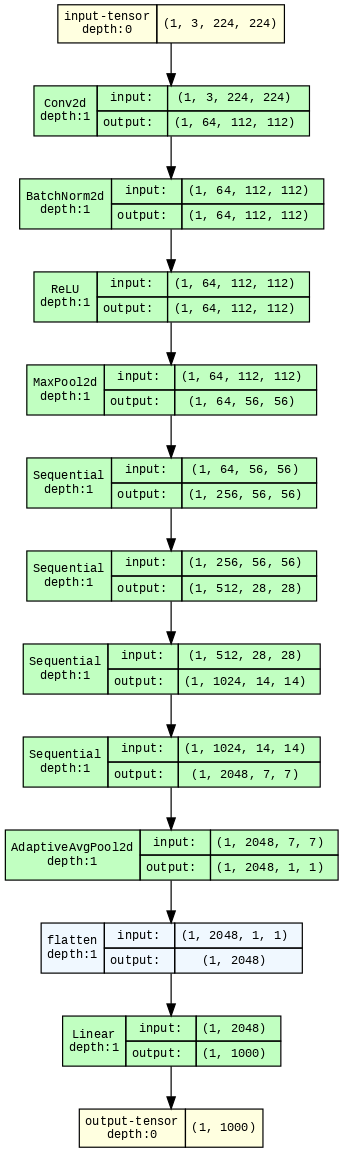
\includegraphics[width=0.4\textwidth]{images/models/ResNet50_overview.png}
    \caption{A ResNet50 szerkezete.}
    \label{fig:ResNet50_overview}
\end{figure}

A \textbf{ResNet50} (Residual Network, 50 réteg mélységű változat) az egyik legmeghatározóbb konvolúciós neurális hálózat, amelyet a Microsoft Research mutatott be 2015-ben a Deep Residual Learning for Image Recognition című tanulmányban \cite{article_resnet50}. Az innováció lényege az ún. \textit{residual blokk}, amely lehetővé teszi a gradiens hatékony terjedését mély rétegeken keresztül.

\paragraph{Működési elve:} A ResNet az identitástér leképezését támogatja azáltal, hogy ún. \textit{skip connection}-öket használ, azaz az inputot változatlanul átadja több rétegen keresztül. Ezzel megelőzi a tanulási nehézségeket, amelyek mély hálók esetén jelentkeznek (pl. gradiens eltűnés, torzulás).

\paragraph{Felépítése:} A ResNet50 50 konvolúciós rétegből áll, melyek \textit{bottleneck} struktúrákba rendeződnek: egy $1\times1$, egy $3\times3$ majd újra egy $1\times1$ konvolúciót tartalmaz minden blokk. Az így kialakított architektúra mély, de mégis hatékonyan tanítható.

\paragraph{Előnyei:}
\begin{itemize}
    \item Rendkívül mély hálózat is stabilan tanítható
    \item Széles körben elérhető előtanított súlyok
    \item Jól működik sokféle feladaton, „baseline”-modellként is tekinthető
\end{itemize}

\paragraph{Hátrányai:}
\begin{itemize}
    \item Nagyobb memóriaigény, főleg inference során
    \item A későbbi, modernebb architektúrákhoz képest nem optimális hatékonyság
\end{itemize}

A ResNet50 tehát egy rendkívül erős és megbízható kiindulópont, amely kiváló összehasonlítási alapként szolgálhat más, újabb modellek értékelésekor.

\subsection{DenseNet121}

\begin{figure}[H]
    \centering
    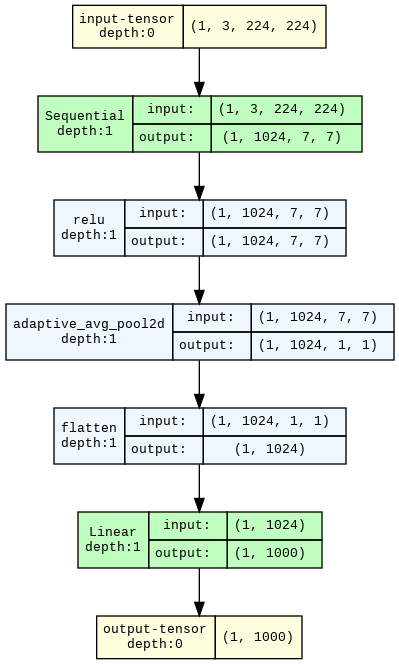
\includegraphics[width=0.4\textwidth]{images/models/DenseNet121_overview.png}
    \caption{A DenseNet121 szerkezete.}
    \label{fig:DenseNet121_overview}
\end{figure}

A \textbf{DenseNet121} (Densely Connected Convolutional Network) szintén egy mély konvolúciós architektúra, amelyet 2017-ben mutattak be \cite{article_densenet}. A DenseNet fő újítása az, hogy minden réteg bemenete az összes korábbi réteg kimenetét is tartalmazza. Ez a „sűrű kapcsolódás” (dense connectivity) elméletileg és gyakorlatilag is javítja az információáramlást és a tanulást.

\paragraph{Működési elve:} A DenseNet nem egyszerűen egymásra épülő rétegeket tartalmaz, hanem minden réteg minden korábbi réteg kimenetét megkapja inputként. Ezáltal az információ és a gradiens nagyon hatékonyan tud terjedni a hálózatban, és kevésbé fordul elő információvesztés.

\paragraph{Felépítése:} A DenseNet121 négy dense blokkot tartalmaz, melyek között ún. \textit{transition} rétegek találhatók, ezek csökkentik a méretet és a csatornaszámot. Az architektúra 121 mély rétegből áll, de a sűrű kapcsolódás miatt a paraméterszáma jóval alacsonyabb, mint a ResNet50-é.

\paragraph{Előnyei:}
\begin{itemize}
    \item Magas hatékonyság kis paraméterszámmal
    \item Kiváló gradiens- és információáramlás
    \item Jó generalizációs képesség, főleg kis adathalmazoknál
\end{itemize}

\paragraph{Hátrányai:}
\begin{itemize}
    \item Lassabb tanítás, mivel sok kapcsolatot kell kezelni
    \item Nagyobb memóriahasználat az összesített rétegbemenetek miatt
\end{itemize}

A DenseNet121 különösen hasznos olyan feladatoknál, ahol fontos a finom részletek megőrzése és hatékony gradiensáramlás, ugyanakkor a paraméterhatékonyság is számít.

\subsection{EfficientNet-B0}

\begin{figure}[H]
    \centering
    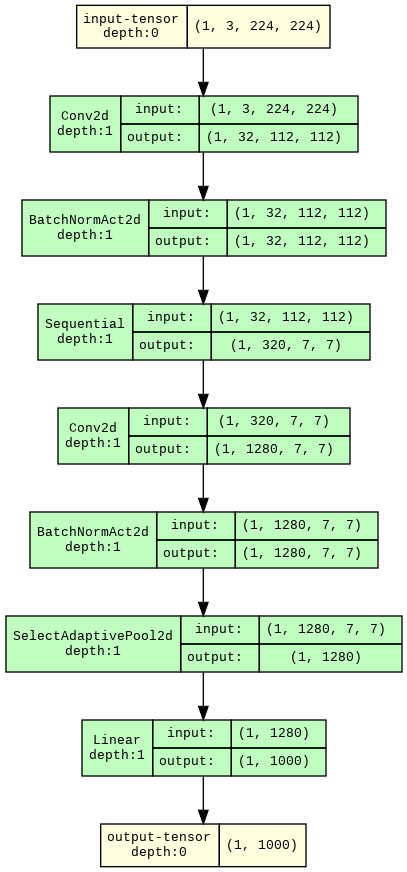
\includegraphics[width=0.4\textwidth]{images/models/EfficientNet-B0_overview.png}
    \caption{A EfficientNet-B0 szerkezete.}
    \label{fig:EfficientNet-B0_overview}
\end{figure}

Az \textbf{EfficientNet-B0} a Google Brain által bemutatott EfficientNet család legalapvetőbb és legkisebb változata \cite{article_efficientnet}. A család célja a hálózati méretezés (scaling) szisztematikus, egységesített megközelítése, amely egyszerre optimalizálja a mélységet, szélességet és felbontást egy ún. „compound scaling” képlettel.

\paragraph{Működési elve:} Ahelyett, hogy egyetlen dimenzió mentén növelnénk a háló méretét (mint pl. csak mélység vagy csak szélesség), az EfficientNet minden dimenziót együtt skáláz a legjobb hatékonyság elérése érdekében. Az alapot egy optimalizált NASNet-féle „mobilbarát” blokk, az \textit{MBConv} adja, amely depthwise separable convolutions-t használ.

\paragraph{Felépítése:} Az EfficientNet-B0 7 MBConv-blokk szintből áll, amelyek kombinálják a bővített konvolúciókat (expansion), depthwise konvolúciót és squeeze-and-excitation (SE) modulokat. Mindez együtt egy kompakt, de rendkívül hatékony architektúrát eredményez.

\paragraph{Előnyei:}
\begin{itemize}
    \item Kiemelkedő pontosság alacsony számítási költségek mellett
    \item Ideális mobil- vagy beágyazott rendszerekre
    \item Modern méretezési elv, amelyet az egész család kiterjeszt
\end{itemize}

\paragraph{Hátrányai:}
\begin{itemize}
    \item Az MBConv blokkok miatt nehezebben értelmezhető, „black-box” jellege lehet
    \item A kis modellváltozatok érzékenyebbek a bemeneti adatok minőségére
\end{itemize}

Az EfficientNet-B0 egy remek választás minden olyan környezetben, ahol fontos a hatékonyság, de nem akarunk kompromisszumot kötni a pontosság terén.

\subsection{ConvNeXt-Tiny}

\begin{figure}[H]
    \centering
    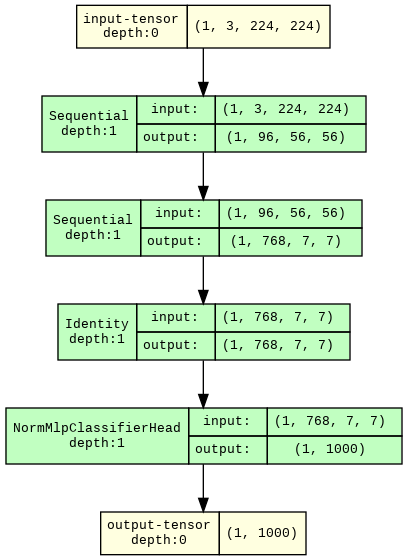
\includegraphics[width=0.4\textwidth]{images/models/ConvNeXt-Tiny_overview.png}
    \caption{A ConvNeXt-Tiny szerkezete.}
    \label{fig:ConvNeXt-Tiny}
\end{figure}

A \textbf{ConvNeXt-Tiny} a 2022-ben bemutatott ConvNeXt architektúra legkisebb változata, amely a konvolúciós neurális hálózatokat (\textit{CNN}) modernizálja a Vision Transformer (ViT) modellek elveinek figyelembevételével \cite{article_convnext}. A cél az volt, hogy újra felélesszék a CNN-ek relevanciáját a transformer-alapú modellek dominanciájával szemben, különösen a számítástechnikai hatékonyság szempontjából.

\paragraph{Működési elve:} A ConvNeXt megőrzi a klasszikus konvolúciós rétegek használatát, de számos architekturális újítást alkalmaz: például normalizációk sorrendje, nagyobb kernelméretek ($7\times7$), LayerNorm használata BatchNorm helyett, és az aktivációk újraértelmezése. Ezek az elemek kombinálva adják az „evolved CNN” karaktert.

\paragraph{Felépítése:} A „Tiny” változat négy szintű hierarchiát alkalmaz, összesen 28 blokkal, és mindössze 28 millió paraméterrel. Az architektúra hatékony és méretében optimalizált, kimondottan jól teljesít kis számítási költségű környezetekben is.

\paragraph{Előnyei:}
\begin{itemize}
    \item Megőrzi a CNN-ek hatékonyságát, de modern ViT-ihlette frissítésekkel
    \item Kompakt modell – gyors tanítás és alacsony memóriaigény
    \item Kimagasló teljesítmény ViT szintjén, de egyszerűbb tanítási folyamat
\end{itemize}

\paragraph{Hátrányai:}
\begin{itemize}
    \item Még viszonylag új architektúra – kevesebb ipari alkalmazás és benchmark
    \item A ViT-nél kisebb képesség a hosszú távú kapcsolatok felismerésére
\end{itemize}

A ConvNeXt-Tiny ideális választás minden olyan feladathoz, ahol a legkorszerűbb CNN-technológia hatékonysága és egyszerűsége is előnyt jelent.

\subsection{ViT-B/16}

\begin{figure}[H]
    \centering
    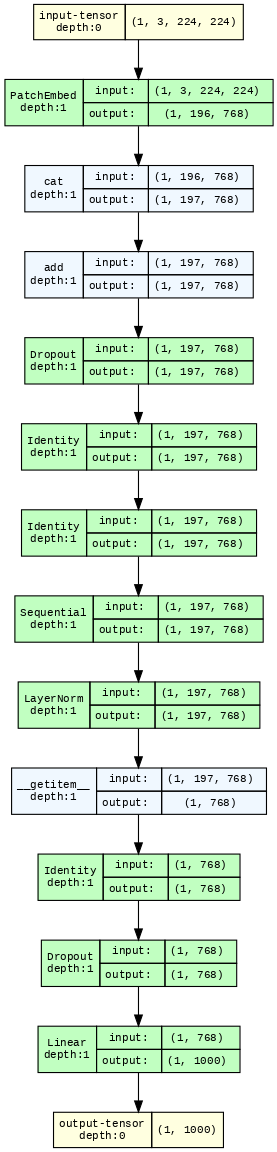
\includegraphics[width=0.2\textwidth]{images/models/ViT-B16_overview.png}
    \caption{A ViT-B/16 szerkezete.}
    \label{fig:B16_overview}
\end{figure}

A \textbf{Vision Transformer Base/16} (röviden \textbf{ViT-B/16}) az első, széles körben elismert \textit{pure transformer} architektúra, amely képeket dolgoz fel a természetes nyelvfeldolgozásban használt transformer architektúra átalakításával \cite{article_vit_b16}. A modell a képeket fix méretű patch-ekre bontja, és ezeket a patch-eket sorozatként kezeli, hasonlóan a szavakhoz egy nyelvi modellben.

\paragraph{Működési elve:} A ViT modellek nem használnak konvolúciókat. Ehelyett a képeket $16\times16$ pixeles foltokra bontják, amelyek lineáris rétegen keresztül kerülnek embed-elésre. Ezután klasszikus transformer encoder blokkok következnek – többfejű figyelemmel (multi-head attention) és feed-forward rétegekkel.

\paragraph{Felépítése:} A ViT-B/16 12 transformer blokkból áll, összesen 86 millió paraméterrel. A „/16” azt jelenti, hogy a bemenet $16\times16$ pixeles foltokra van osztva. A képeket egy „class token” egészíti ki, amelyre a végső predikció épül.

\paragraph{Előnyei:}
\begin{itemize}
    \item Kiváló hosszú távú kapcsolat-érzékelő képesség
    \item Skálázhatóság – nagyobb modellekkel arányosan nő a teljesítmény
    \item Egyszerű, elegáns architektúra konvolúciók nélkül
\end{itemize}

\paragraph{Hátrányai:}
\begin{itemize}
    \item Nagy adatmennyiséget igényel a hatékony tanuláshoz
    \item Lassabb konvergencia, érzékenyebb a hiperparaméterekre
    \item Kevésbé hatékony kis modellek és kisebb adathalmazok esetén
\end{itemize}

A ViT-B/16 segítségével összehasonlítható, hogy a „pure attention” alapú modellek hogyan teljesítenek a klasszikus és új generációs CNN-ekhez képest.

\subsection{Inception-v3}

\begin{figure}[H]
    \centering
    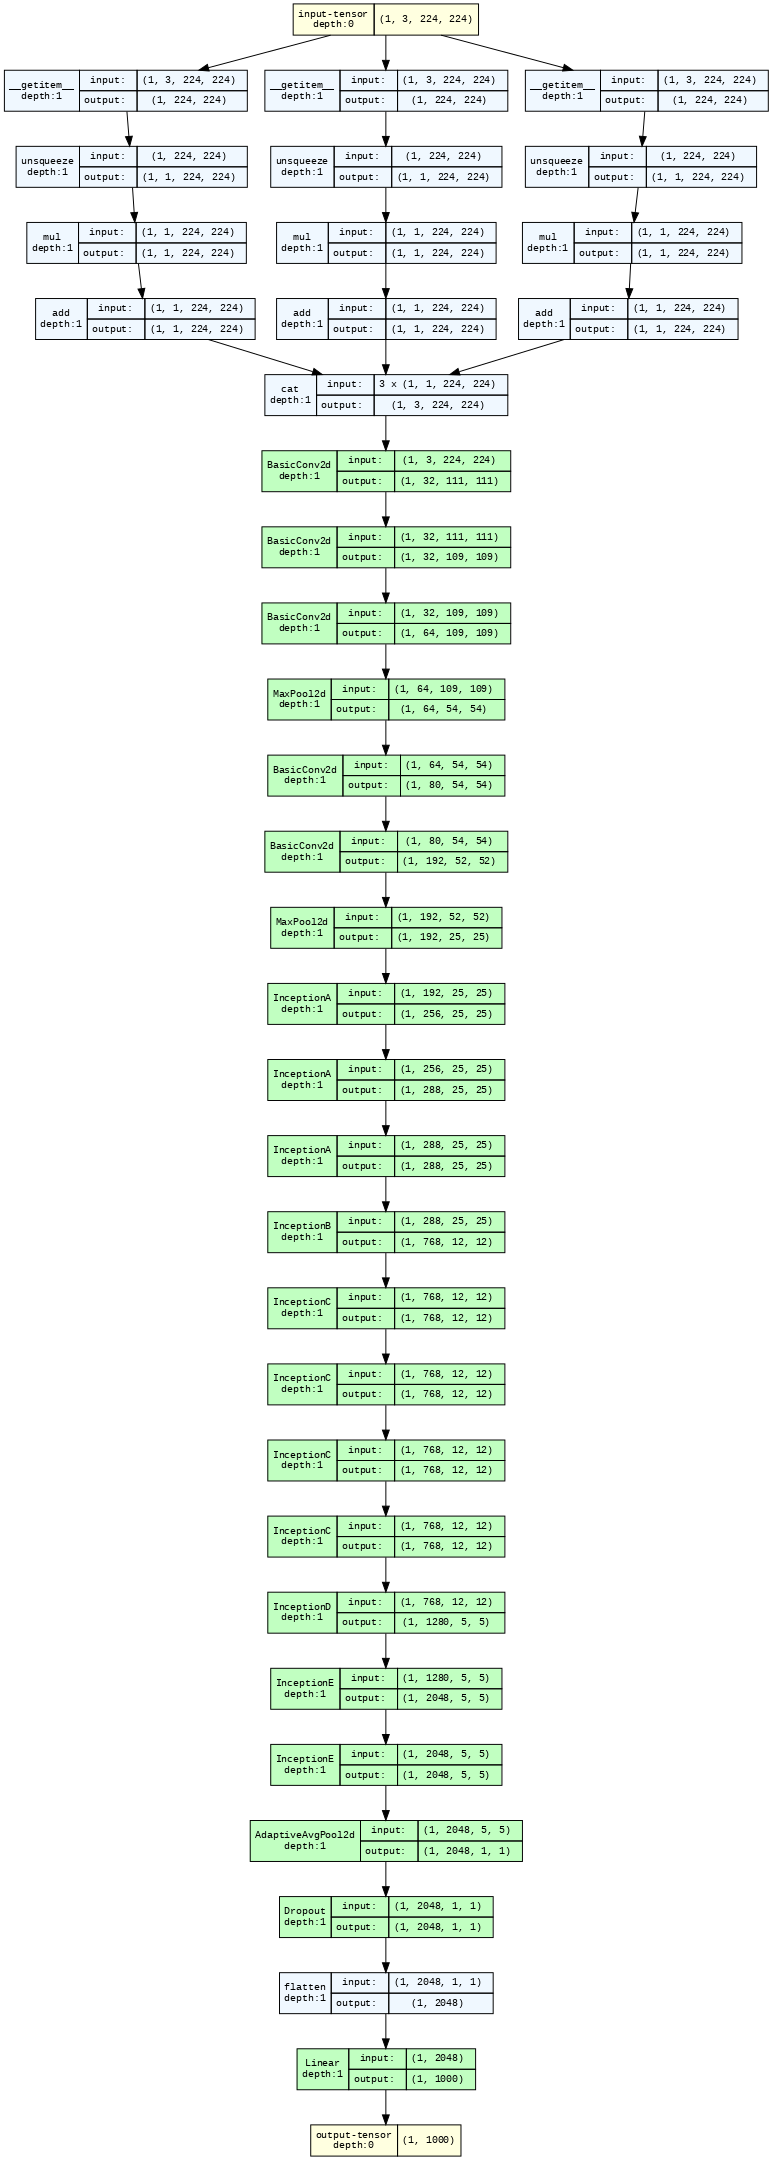
\includegraphics[width=0.35\textwidth]{images/models/Inception-v3_overview.png}
    \caption{A Inception-v3 szerkezete.}
    \label{fig:Inception-v3_overview}
\end{figure}

Az \textbf{Inception-v3} a Google által fejlesztett Inception-sorozat egyik legnépszerűbb és legsikeresebb verziója, amelyet 2015-ben mutattak be \cite{article_inception_v3}. A fő cél a számítási hatékonyság növelése anélkül, hogy csökkenne a pontosság. Az architektúra újdonsága az Inception-modul, amely különböző méretű konvolúciókat párhuzamosan futtat, így több skálán is képes információt kinyerni.

\paragraph{Működési elve:} Az Inception-v3 egy összetett architektúra, amelyben a konvolúciós rétegeket párhuzamosan, különböző szűrőméretekkel (pl. $1\times1$, $3\times3$, $5\times5$) alkalmazzák, és ezek kimenetét egyesítik. Ez lehetővé teszi a hatékony, mély és széles jellemzők kinyerését különböző felbontásokon.

\paragraph{Felépítése:} A hálózat több Inception-modulból áll, melyek között redukciós (méretcsökkentő) blokkok találhatók. A teljes modell körülbelül 24 millió paraméterből áll, ami viszonylag kis szám az akkori modellekhez képest.

\paragraph{Előnyei:}
\begin{itemize}
    \item Hatékony architektúra – kevesebb paraméter, mégis magas pontosság
    \item Több skálán történő reprezentációtanulás
    \item Jó választás korlátozott erőforrások mellett is
\end{itemize}

\paragraph{Hátrányai:}
\begin{itemize}
    \item Bonyolultabb architektúra, nehezebb reprodukálni
    \item A későbbi modellek hatékonyabban kihasználják a modern hardvereket
\end{itemize}

Az Inception-v3 egy történetileg fontos, hatékony CNN-architektúra, amely értékes összehasonlítási alap a modernebb, komplexebb modellekhez képest.

\subsection{NASNet}

\begin{figure}[H]
    \centering
    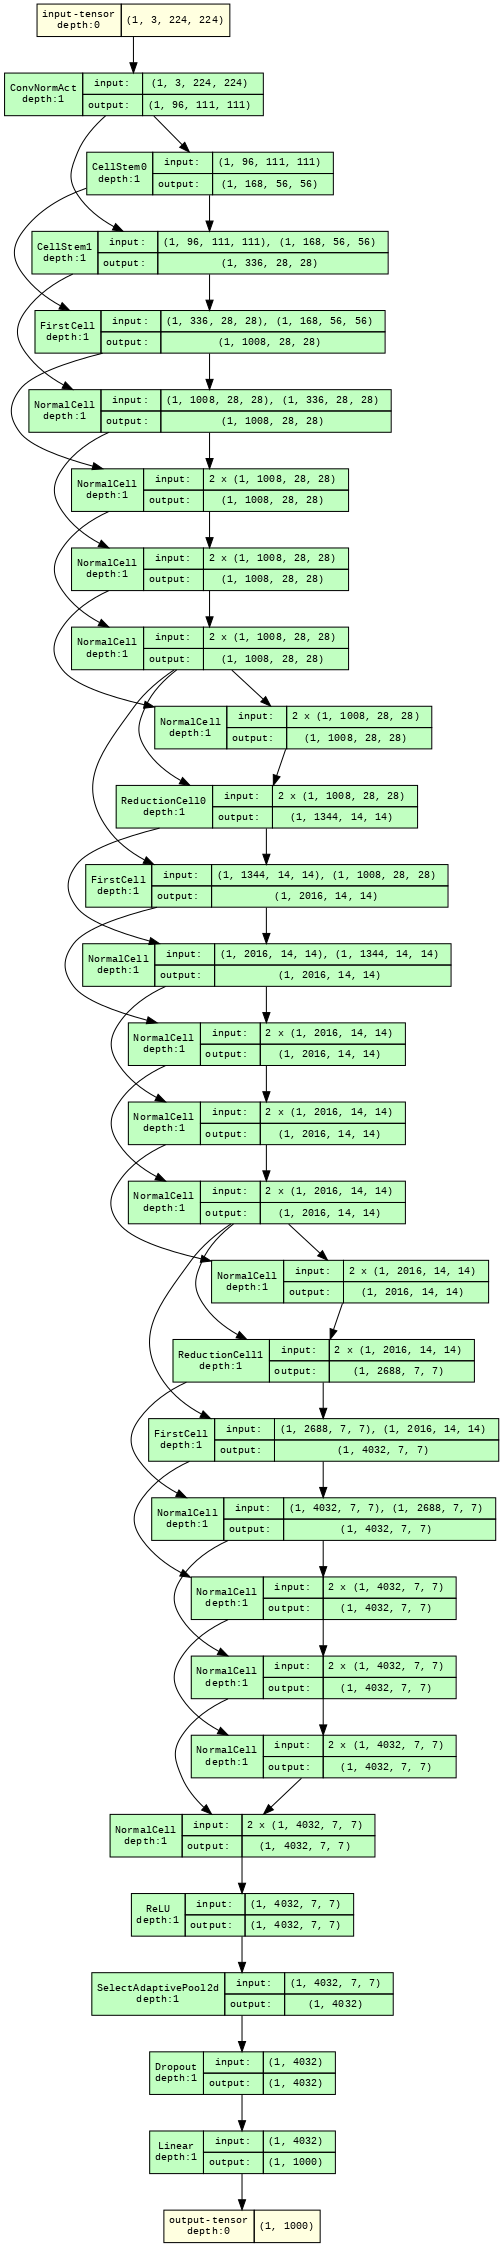
\includegraphics[width=0.25\textwidth]{images/models/NASNet_overview.png}
    \caption{A NASNet szerkezete.}
    \label{fig:NASNet_overview}
\end{figure}

A \textbf{NASNet} (Neural Architecture Search Network) egy olyan architektúra, amelyet nem ember, hanem gépi tanulás által optimalizált keresőalgoritmus (NAS – Neural Architecture Search) hozott létre. A Google AutoML csapata mutatta be 2018-ban \cite{article_nasnet}. A cél az volt, hogy automatikusan találjanak kiemelkedően teljesítő neurális hálóarchitektúrákat.

\paragraph{Működési elve:} A NASNet modulokat kis, ismétlődő „cellákra” bontják: egy „normal cell”-re és egy „reduction cell”-re. Ezeket egy keresőalgoritmus iteratívan optimalizálja egy kisebb adathalmazon (pl. CIFAR-10), majd a végső architektúrát átméretezik a célfeladathoz (pl. ImageNet).

\paragraph{Felépítése:} A NASNet nagyméretű, moduláris modell, amely tipikusan 88 millió paramétert tartalmaz a „NASNet-A Large” változatban, de léteznek kisebb, mobilos verziók is (pl. NASNet-Mobile).

\paragraph{Előnyei:}
\begin{itemize}
    \item Automatikus optimalizálás – gyakran jobb eredmények emberi tervezés nélkül
    \item Moduláris, skálázható architektúra
    \item Jó teljesítmény mind számításigényes, mind mobil környezetben
\end{itemize}

\paragraph{Hátrányai:}
\begin{itemize}
    \item Komplex tanítási folyamat – a NAS futtatása rendkívül erőforrás-igényes
    \item Nehezebben interpretálható, mint a kézzel tervezett modellek
\end{itemize}

A NASNet betekintést enged az architektúra-keresésen alapuló modern modellek világába, és összehasonlítási lehetőséget nyújt az ember által tervezett modellekkel szemben.


\section{A kiválasztott metrikák}

A modellek kiértékelése során olyan metrikák alkalmazása szükséges, amelyek átfogó és megbízható képet adnak a tanítás hatékonyságáról, a generalizációs képességekről, valamint az adott feladathoz való illeszkedésről. A kiválasztott metrikák jól bevált, nemzetközileg elismert szabványok a számítógépes látás és osztályozási feladatok körében. A következőkben részletesen ismertetem ezen metrikák jelentését és indoklását.

\subsection{Top-1 pontosság}

A \textbf{Top-1 pontosság} azt méri, hogy a modell legnagyobb valószínűséggel megjósolt osztálya megegyezik-e a valódi címkével. Ez a leggyakoribb és legegyszerűbb értékelési mód képosztályozási feladatok esetén. Különösen fontos, amikor a cél az, hogy a modell első próbálkozásra pontosan eltalálja a helyes kategóriát.

\textit{Miért választottam?}  
Mivel az alkalmazás célja pontos osztályozás, ezért elengedhetetlen látni, hogy az elsődleges (legvalószínűbb) predikciók milyen mértékben feleltethetők meg a valóságos címkéknek.

\subsection{Top-5 pontosság}

A \textbf{Top-5 pontosság} azt vizsgálja, hogy a modell által megjósolt öt legvalószínűbb kategória között szerepel-e a helyes válasz. Ezt gyakran használják olyan osztályozási problémáknál, ahol sok a hasonló kategória (pl. madárfajok, járműtípusok), és a teljesen pontos becslés helyett a „jó irány” is informatív.

\textit{Miért választottam?}  
Mivel az SBphotoThemes180K adathalmazban számos átfedő és vizuálisan hasonló kategória található, a Top-5 pontosság segít feltárni, ha a modell ugyan nem találja el elsőre a helyes kategóriát, de erősen közelíti azt.

\subsection{Precision}

A \textbf{precision} (pozitív predikciós érték) megmutatja, hogy az adott osztályra vonatkozóan a modell által „pozitívnak” vélt találatok közül hány volt valóban helyes. Ez fontos ott, ahol a téves pozitív eredmények költségesek lehetnek.

\textit{Miért választottam?}  
Ez a metrika különösen hasznos annak vizsgálatára, hogy mennyire „megalapozottak” a modell predikciói: azaz, ha a modell valamit „biztosra” mond, az milyen arányban bizonyul igaznak.

\subsection{Recall}

A \textbf{recall} (érzékenység) azt mutatja meg, hogy az adott osztályba tartozó valódi példányok közül mennyit ismer fel a modell. Ez akkor fontos, ha nem akarunk elvéteni fontos eseteket (pl. egészségügyi vagy biztonsági alkalmazásokban).

\textit{Miért választottam?}  
Segít annak feltérképezésében, hogy a modell mennyire képes felismerni az adott osztályba tartozó képeket, még akkor is, ha azok eltérnek a tipikus mintától.

\subsection{F1-score}

Az \textbf{F1-score} a precision és a recall harmonikus átlaga. Ez kiegyensúlyozott mérőszám, amely akkor is informatív, ha a két előző mutató eltérő tendenciát mutat.

\textit{Miért választottam?}  
Az F1-score révén egyetlen értékben kaphatunk képet a modell általános osztályozási képességéről, figyelembe véve mind a túlzott pozitív predikciókat, mind a kihagyott eseteket.

\subsection{Train és Val loss}

A \textbf{train loss} és a \textbf{validation loss} a modell tanítása során keletkező veszteség (loss function értéke) alakulását mutatja. A train loss a tanítóhalmazon, míg a val loss az ismeretlen validációs adatokon mért érték.

\textit{Miért választottam?}  
Ezek elengedhetetlen metrikák a tanulási folyamat nyomon követéséhez. A két görbe összehasonlításával feltárható a modell túlilleszkedése (\textit{overfitting}) vagy alulilleszkedése (\textit{underfitting}).

\subsection{Train és Val pontosság}

A \textbf{train accuracy} és a \textbf{validation accuracy} megmutatják, hogy a modell milyen arányban jósolja meg helyesen a címkéket a tanító, illetve a validációs halmazon. Ezek értéke szorosan összefügg a loss értékekkel, de intuitívabbak és könnyebben értelmezhetők.

\textit{Miért választottam?}  
A pontosság segít vizuálisan és numerikusan követni a tanítás sikerességét. Az eltérés a tanító és a validációs pontosság között utalhat az általánosító képesség hiányosságaira.

\section{Összegzés}

Ebben a fejezetben részletesen bemutattam azokat a mélytanulási modelleket, amelyeket az SBphotoThemes180K adathalmaz osztályozási teljesítményének értékelésére kiválasztottam. A modellek között megtalálhatók a klasszikus konvolúciós architektúrák, mint a ResNet50 és az Inception-v3, a paraméterhatékonyságra optimalizált megközelítések, mint az EfficientNet-B0 és a NASNet, valamint a korszerűbb, transzformer-alapú ViT-B/16 modell és a ConvNeXt, amely a modern ViT-hatásokkal bővített konvolúciós architektúrák új hullámát képviseli.

A modellek kiválasztását indokolja az, hogy különböző architekturális iskolákat képviselnek, eltérő számítási igénnyel, parametrikus komplexitással és általánosító képességgel rendelkeznek. Ez lehetővé teszi a mély tanulási megközelítések közötti összehasonlítást egy viszonylag nagy, valóságból származó képadatbázison.

A teljesítmény értékeléséhez használt metrikák szintén tudatos választás eredményei: a Top-1 és Top-5 pontosság alapvető osztályozási mutatók, míg a Precision, Recall és F1-score lehetővé teszik az egyensúlyi hibák feltérképezését, különösen sokosztályos feladatoknál. A tanulási folyamat megértéséhez és optimalizálásához pedig a loss és pontosság alakulásának idősoros vizsgálata szolgál alapul.

Ezen modellek és metrikák együttes vizsgálata biztosítja, hogy a későbbi fejezetekben bemutatott kísérleti eredmények nemcsak technikai szempontból megalapozottak, hanem mélyebb következtetések levonására is alkalmasak a modellválasztás, az architektúra-hatékonyság, valamint az adathalmaz minőségének és nehézségi szintjének szempontjából.

\chapter{Vizsgálati metodika}

\section{A mérési környezet}
  A méréseket Google Colab Pro környezetben végeztem el Colab (Jupyter) notebook-ok segítségével Python nyelven CUDA gyorsítással. Az adatbázis építése az automatikus rendezés kivételével (ami Colab-on történt) lokálisan történt python és shell szkriptek segítségével. 

  \subsection{Az alkalmazott grafikus kártyák}
  \begin{itemize}
    \item NVIDIA A100-SXM4-40GB
    \item NVIDIA L4 GPU
  \end{itemize}
  Az esetek többségében az L4 GPU-t használtam, ez óránként 2 számítási egységet használt fel, így gazdaságosabb volt. A különsen számításigényes tanításokhoz alkalmaztam az A100 GPU-t a sebessége miatt, de az 8 számítási egyéget fogyasztott óránként, így költséges volt használni. 
  \note{
  Az Inference time és az Epoch iterációs idő a két időérzékeny mérési eredmény, ilyenkor az alkalmazott GPU feltüntetésre kerül.
  }

\subsection{Az alkalmazott szoftveres környezet}
  A méréseket Google Colab Pro környezetben végeztem el Colab (Jupyter) notebook-ok segítségével Python nyelven CUDA gyorsítással. Az adatbázis építése az automatikus rendezés kivételével lokálisan történt python és shell szkriptek segítségével. 
  Az elkészített mérési és adatbázis építő szoftver a mellékelt tömörített fájlban, vagy a projekt Github repository-jában található.
  A szoftverek működésének ismeretése a Melléklet B: Elkészített szoftverek részben található.
  note {A "k" rövidítés a kilo mint ezer jelölésére szolgál}

  \section{Mérésmetodika}

  A mérési metodika célja, hogy különböző mélytanulási modellek képességeit objektíven, összehasonlítható módon vizsgálja egy egységes, valóságból származó, sokosztályos képadatbázison. A kiválasztott modellek sokfélesége (klasszikus konvolúciós hálók, hatékonyságra optimalizált architektúrák, transzformer-alapú modellek) megköveteli, hogy az értékelés többdimenziós és fokozatosan mélyülő legyen.
  
  A vizsgálat során két osztályozás került előállításra az SBphotoThemes180K adathalmazon:
  \begin{itemize}
    \item \textbf{ImageNet1k osztályozás}: 114 kategóriába sorolt képek – ez a vizsgálatok fő fókusza.
    \item \textbf{Places365 osztályozás}: 121 kategória – ez jövőbeli kutatások alapja lesz.
  \end{itemize}
  
  Az adatbázis három részre lett osztva:
  \begin{itemize}
    \item \textbf{Train (80\%)}: 144600 kép – a tanítási adathalmaz.
    \item \textbf{Validation (10\%)}: 18075 kép – a validációs teljesítmény mérése a tanítás alatt.
    \item \textbf{Test (10\%)}: 18075 kép – minden mérés azonos, változatlan teszthalmazon történt.
  \end{itemize}
  
  A méréseket négy, külön célt szolgáló fázisban hajtottam végre. Mindegyik fázis eltérő megközelítést képvisel, és más-más szempontból szolgáltat információt a modellek viselkedéséről.
  
  %---
  
  \section{I. Fázis: Tanítás nélküli tesztelés}
  
  Ebben a fázisban minden kiválasztott modellt úgy teszteltem a teljes teszthalmazon, hogy nem történt semmiféle finomhangolás vagy tanítás – vagyis a modellek előtanított állapotban, az ImageNet súlyokkal kerültek kiértékelésre.
  
  \textbf{Cél:} A kiindulási teljesítmény meghatározása, amely megmutatja, hogy a modellek milyen mértékben képesek generalizálni az új, de hasonló doménből származó képekre a tanítás nélkül.
  
  \textbf{Jelentősége:}
  \begin{itemize}
    \item Segít megérteni, mennyire adaptálható egy adott modell nulladik lépésben.
    \item Alapvető referenciaértékeket biztosít a későbbi tanítások eredményének értelmezéséhez.
    \item Fény derülhet arra, hogy bizonyos architektúrák már a pre-trainelt állapotban is előnyt élveznek.
  \end{itemize}
  
  Ez különösen fontos volt az SBphotoThemes180K adathalmaz esetén, mivel az osztályok egy része átfedést mutat az ImageNet1k alap kategóriáival.
  
  %---
  
  \section{II. Fázis: Teljes tanítás}
  
  Ebben a fázisban minden modellt teljesen betanítottam a teljes 144600 képet tartalmazó tanítóhalmazon. A tanítás során 10 epochon keresztül zajlott a modell optimalizálása, kivéve a NASNet modellt, ahol a számítási kapacitás korlátai miatt csak 2 epochig tartott a tréning.
  
  \textbf{Cél:} A modellek maximális, hosszú távú tanulási potenciáljának feltérképezése az egész adathalmazon.
  
  \textbf{Jelentősége:}
  \begin{itemize}
    \item Megmutatja, hogyan képesek a modellek a teljes adathalmaz információtartalmát kihasználni.
    \item Objektív összehasonlítást nyújt a különböző architektúrák generalizációs és tanulási képességeiről.
    \item Részletes metrikák (Top-1, Top-5, Precision, Recall, F1, Train/Val loss) segítségével pontosan mérhető a tanulás dinamikája.
  \end{itemize}
  
  A tanítás után minden modell ugyanazon a teszthalmazon került kiértékelésre, így közvetlen összehasonlítás vált lehetővé.
  
  %---
  
  \section{III. Fázis: Iteratív tanítás}
  
  Ebben a vizsgálati lépésben azt kutattam, hogyan alakul a modellek teljesítménye különböző méretű tanítóhalmazok mellett. Minden modell négy lépésben tanult: 1k, 5k, 10k, és 25k méretű tanítóhalmazokon, külön-külön. Minden esetben 10 epochon keresztül történt a tréning, kivéve a NASNet esetében, ahol az erőforrásigények miatt csökkentett epoch számokat alkalmaztam.
  
  \textbf{Cél:} A modellek tanulási görbéjének és érzékenységének vizsgálata eltérő adatmennyiség mellett.
  
  \textbf{Jelentősége:}
  \begin{itemize}
    \item Segít meghatározni, mely modellek tanulnak hatékonyan már kisebb adathalmazon is.
    \item Rávilágít a modellek adatéhségére és generalizációs képességeire az adatméret függvényében.
    \item Lehetővé teszi a modellválasztás optimalizálását korlátozott adatkészletek esetén.
  \end{itemize}
  
  Az iteratív mérések alapján tanulási görbék és részletes statisztikai kimutatások készültek, amelyek jól szemléltetik az architektúrák különbségeit a korai fázisú tanulásban.
  
  %---
  
  \section{IV. Fázis: Saját modell fejlesztése}
  
  A méréssorozat negyedik fázisában saját, egyedileg kialakított modell kifejlesztésére és kiértékelésére került sor, a korábbi eredmények és tanulságok alapján.
  
  \textbf{Cél:} Egy hatékony, célzottan az SBphotoThemes180K adathalmazhoz optimalizált neurális háló létrehozása.
  
  \textbf{Jelentősége:}
  \begin{itemize}
    \item A vizsgálatok tapasztalataira építve lehetőség nyílik egy könnyű, mégis pontos osztályozó modell kialakítására.
    \item Az egyedi modell összehasonlítása a „nagy” modellekkel segít feltárni, hogy az adaptált architektúrák mikor tudnak versenyképesek lenni.
    \item Az ilyen fejlesztések irányt mutathatnak jövőbeli alacsony számítási igényű, valós idejű alkalmazások számára.
  \end{itemize}
  
  Ez a fázis különösen fontos abban az esetben, ha a cél egy deployálható, hatékony rendszer létrehozása, nem csupán kutatási célú összehasonlítás.
  
  %---
  

\chapter{Szoftveres környezet}
    A gördülékeny munkához minden lépéshez saját egyedi szoftvereket kellett készítenem. Ezek érdekesebb részleteit kiemelem a következőkben, teljes terjedelmében a projekt GitHub repository-jában érhetőek el, bővebben pedig a mellékletben.

    \section{A mérési környezet}
    A méréseket Google Colab Pro környezetben végeztem el Colab (Jupyter) notebook-ok segítségével Python nyelven CUDA gyorsítással. Az adatbázis építése az automatikus rendezés kivételével (ami Colab-on történt) lokálisan történt python és shell szkriptek segítségével. 
  
    \subsection{Az alkalmazott grafikus kártyák}
    \begin{itemize}
      \item NVIDIA A100-SXM4-40GB
      \item NVIDIA L4 GPU
    \end{itemize}

    Az esetek többségében az L4 GPU-t használtam, ez óránként 2 számítási egységet használt fel, így gazdaságosabb volt. A különsen számításigényes tanításokhoz alkalmaztam az A100 GPU-t a sebessége miatt, de az 8 számítási egyéget fogyasztott óránként, így költséges volt használni.

    \note{
    Az Inference time és az Epoch iterációs idő a két időérzékeny mérési eredmény, ilyenkor az alkalmazott GPU feltüntetésre kerül.
    }
  
  \subsection{Az alkalmazott szoftveres környezet}
    A méréseket Google Colab Pro környezetben végeztem el Colab (Jupyter) notebook-ok segítségével Python nyelven CUDA gyorsítással. Az adatbázis építése az automatikus rendezés kivételével lokálisan történt python és shell szkriptek segítségével. 
    Az elkészített mérési és adatbázis építő szoftver a mellékelt tömörített fájlban, vagy a projekt Github repository-jában található.
    A szoftverek működésének ismeretése a Melléklet B: Elkészített szoftverek részben található.

    \section{Lokális vagy Online környezet}
        A vizsgálat során döntő kérdés volt, hogy a mérések és modellfuttatások lokális gépen vagy felhőalapú (online) környezetben történjenek. A rendelkezésre álló lokális hardver nem tette lehetővé nagy számításigényű neurális hálók (pl. NASNet vagy ViT-B/16) hatékony betanítását, különösen többféle konfiguráció és adathalmaz-összeállítás mellett.

        A modellek tanítása során a memóriaigény gyakran meghaladta a 10-16 GB GPU memóriát, amihez lokálisan nem állt rendelkezésre megfelelő NVIDIA grafikus kártya. Emellett a hosszú tanítási idők (akár több óra/modell) a gép folyamatos elérhetőségét igényelték volna, amit egy nem dedikált kutatói workstation nem tudott garantálni.
        
        Ezért az online, skálázható és CUDA-gyorsított környezetet biztosító Google Colab Pro megoldást választottam. Ez lehetővé tette a mérések párhuzamos, hatékony elvégzését és a különösen számításigényes szakaszokhoz rugalmasan erősebb GPU-k igénylését.

    \section{Google Colab lehetőségek}
        A Google Colab Pro környezet többféle GPU-típushoz biztosít hozzáférést, köztük olyan erős architektúrákhoz, mint az NVIDIA A100 és L4. Ezek a kártyák a modern neurális hálózati modellekhez tervezett csúcshardverek, és kiválóan alkalmasak mélytanulási feladatokra.

        A Colab lehetővé teszi a Jupyter notebook-ok futtatását felhőben, közvetlenül Python nyelven. A Colab Pro előfizetéssel gyakrabban és hosszabb ideig érhetők el a prémium GPU-k, ez döntő fontosságú volt a 10 epoch-os betanításokhoz és az iteratív tanulási vizsgálatokhoz.
        
        A két alkalmazott GPU jellemzői:
            \begin{itemize}          
            \item NVIDIA L4 GPU: Gazdaságosabb, de modern architektúra, főként inference célokra optimalizálva. Egy Colab számítási egységből két L4 GPU-használati órát lehetett lefedni, így ez volt a fő választásom a kisebb modellekhez és gyorsabb kísérletekhez.
        
            \item NVIDIA A100-SXM4-40GB: Az egyik legerősebb, kutatásokhoz tervezett GPU. Kiemelkedő teljesítménye miatt az A100-at a legnagyobb modellek (pl. NASNet, ViT) tanításához és az időkritikus benchmarkok futtatásához alkalmaztam. Ugyanakkor egy A100-óra 8 számítási egységet igényelt, ezért korlátozottan volt használható.
            \end{itemize}
        
        A Colab környezet automatizálható, újraindítható, és kódosztással dokumentálható – ez a dolgozat replikálhatósága és nyíltsága szempontjából is előnyös volt.

    \section{Tárolási problémák}
        A teljes adathalmaz mintegy 180 750 darab 224x224-es JPEG kép volt, ami tömörítve is több gigabájtos állományt jelentett. A Google Colab felhasználói fiókjához csak korlátozott méretű ideiglenes tároló kapcsolódik (12-15 GB), ami nem volt elegendő a teljes adathalmaz kitömörített formában történő használatához.

        A probléma megoldásához a képeket csoportosított ZIP-állományokba rendeztem, amelyeket a Google Drive-on tároltam. A Colab notebook a mérés kezdetén ezeket a ZIP fájlokat lokálisan, szakaszosan csomagolta ki, csak az éppen szükséges adatokkal dolgozva. Ez a módszer:
        \begin{itemize}
            \item megkerülte a fájlrendszer méretkorlátját,
        
            \item biztosította a Colab és Google Drive közötti gyors adatelérést,
        
            \item lehetővé tette az adathalmaz többlépcsős tanításához szükséges szelektív betöltést.
        \end{itemize}
        A megközelítés nemcsak hatékony, de rugalmas is volt.




\chapter{I. Fázis: Tanítás nélküli tesztelés}
    Ebben a fázisban minden kiválasztott modellt úgy teszteltem a teljes teszthalmazon, hogy nem történt semmiféle finomhangolás vagy tanítás – vagyis a modellek előtanított állapotban, az ImageNet súlyokkal kerültek kiértékelésre.
    
    \textbf{Cél:} A kiindulási teljesítmény meghatározása, amely megmutatja, hogy a modellek milyen mértékben képesek generalizálni az új, de hasonló doménből származó képekre a tanítás nélkül.

    \section{ResNet50}
        \begin{center}
        \begin{longtable}{l c}
        \caption{ResNet50 tanítás nélküli vizsgálat eredményei} \label{tab:phase01_ResNet50} \\
        \toprule
        \textbf{Metrika} & \textbf{Érték} \\
        \midrule
        \endfirsthead
        \toprule
        \textbf{Metrika} & \textbf{Érték} \\
        \midrule
        \endhead
        Top-1 Accuracy & 0.4698 \\
        Top-5 Accuracy & 0.7962 \\
        Precision & 0.3934 \\
        Recall & 0.3797 \\
        F1-score & 0.3592 \\
        Inference time & 25.21 sec \\
        \bottomrule
        \end{longtable}
        \end{center}

        \subsubsection{ResNet50 tanítás nélküli normalizált Confusion Mátrix}
        \begin{figure}[H]
        \centering
        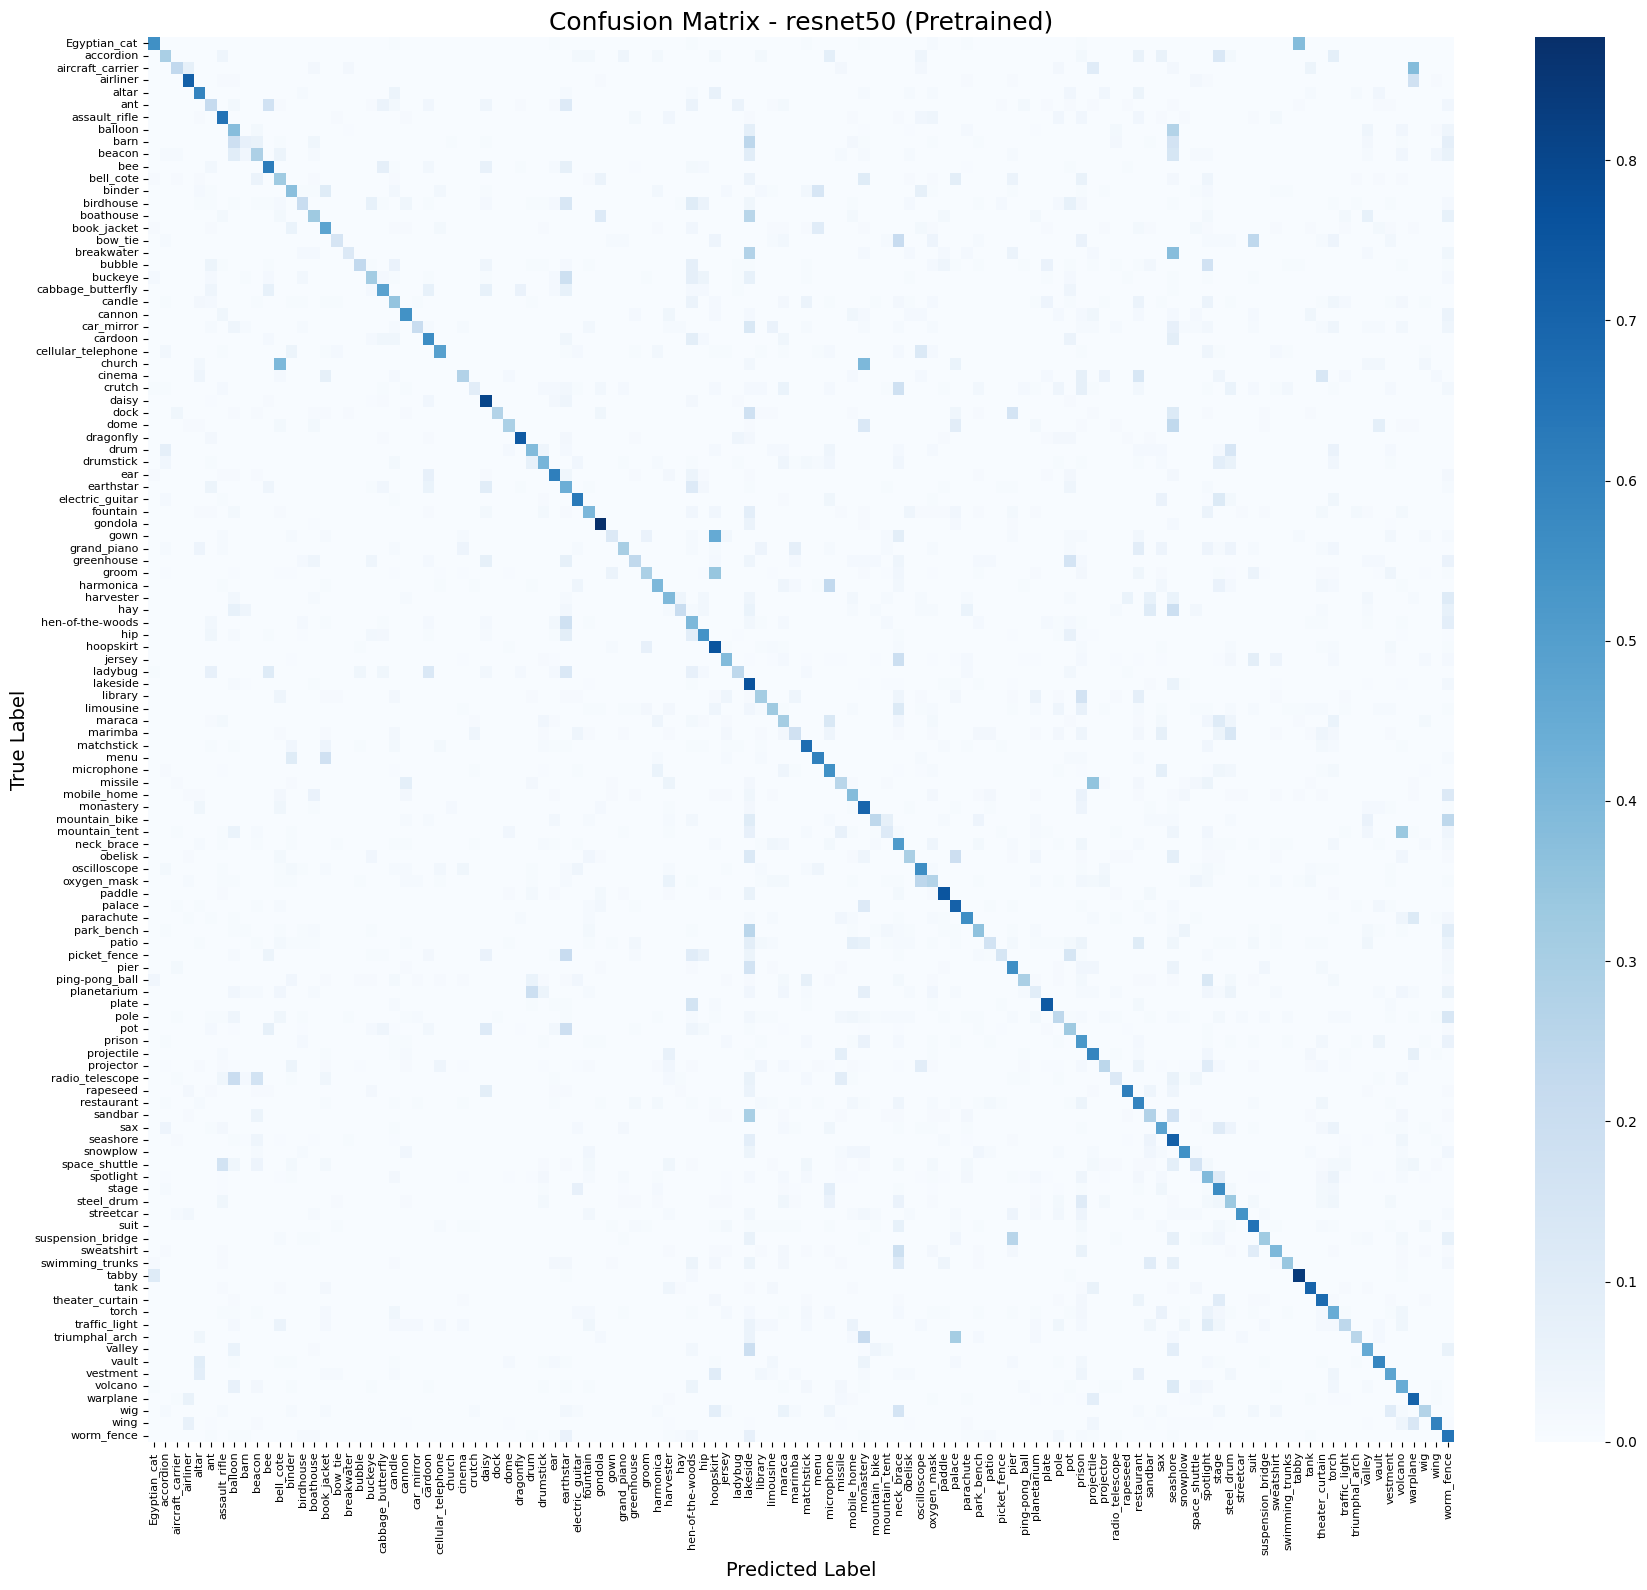
\includegraphics[width=0.8\textwidth]{images/phase01/ResNet50_normalised_conf_mat.png}
        \caption{ResNet50 tanítás nélküli normalizált Confusion Mátrix}
        \label{fig:phase01_ResNet50_normalised_conf_mat}
        \end{figure}

    \section{DenseNet121}
        \subsubsection{DenseNet121 tanítás nélkül teszt}
        \begin{center}
        \begin{longtable}{lc}
        \caption{DenseNet121 @ ImageNet1k tanítás nélküli vizsgálat eredményei}%
        \label{tab:phase01_DenseNet121} \\
        \toprule
        \textbf{Metrika} & \textbf{Érték} \\
        \midrule
        \endfirsthead
        \toprule
        \textbf{Metrika} & \textbf{Érték} \\
        \midrule
        \endhead
        Top-1 Accuracy & 0.4498 \\
        Top-5 Accuracy & 0.7806 \\
        Precision & 0.3874 \\
        Recall & 0.3611 \\
        F1-score & 0.3408 \\
        Inference time & 25.15 sec \\
        \bottomrule
        \end{longtable}
        \end{center}

        \subsubsection{DenseNet121 tanítás nélküli normalizált Confusion Mátrix}
        \begin{figure}[H]
            \centering
            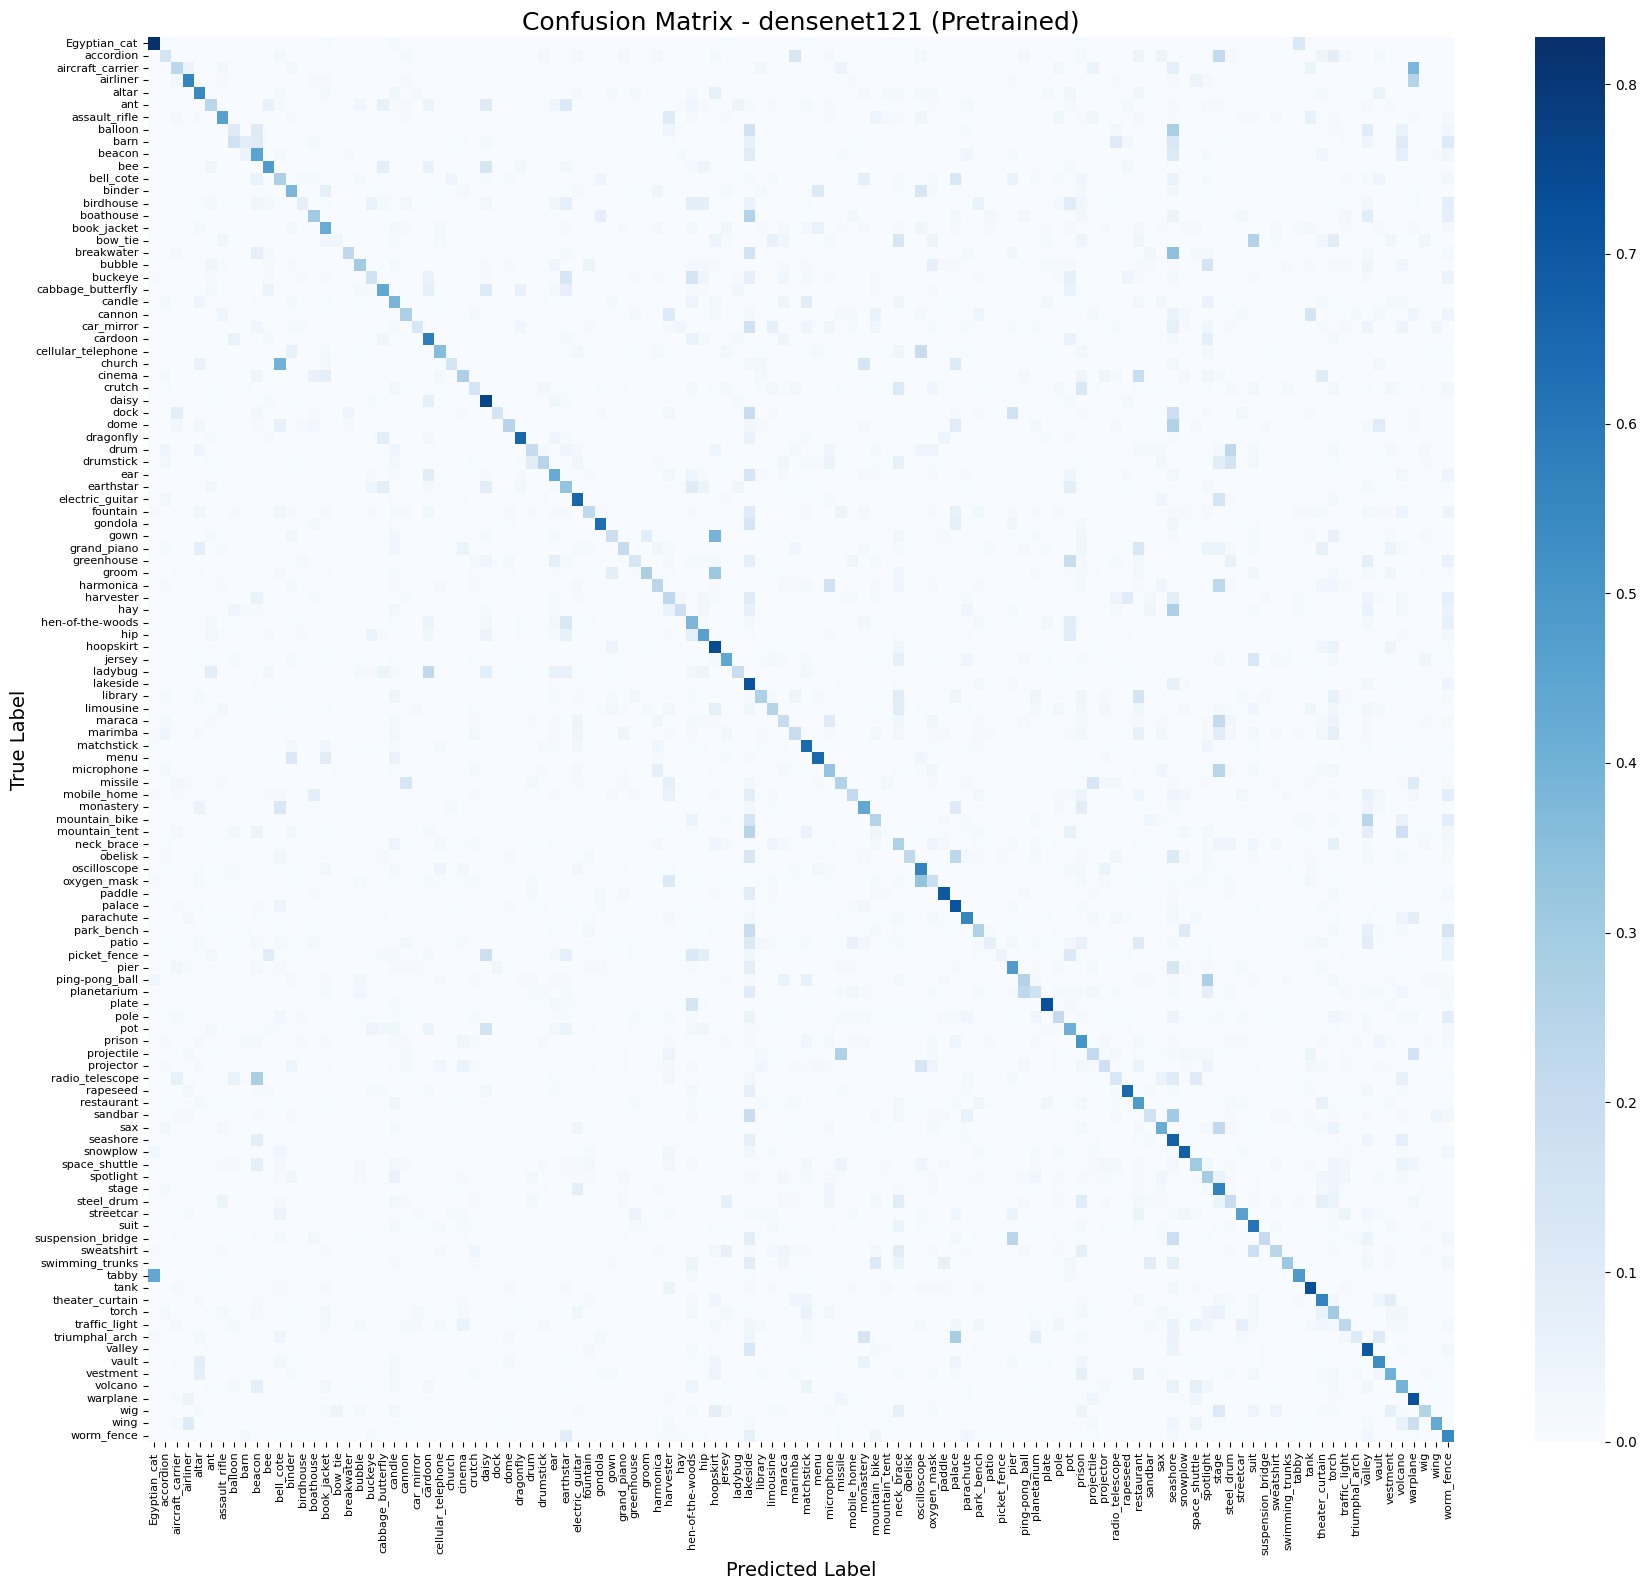
\includegraphics[width=0.8\textwidth]{images/phase01/DenseNet121_normalised_conf_mat.png}
            \caption{DenseNet121 tanítás nélküli normalizált Confusion Mátrix}
            \label{fig:phase01_DenseNet121_normalised_conf_mat}
        \end{figure}

    \section{EfficientNet-B0}
        \subsubsection{EfficientNet-B0 tanítás nélkül teszt}
        \begin{center}
        \begin{longtable}{l c}
        \caption{EfficientNet-B0 tanítás nélküli vizsgálat eredményei} \label{tab:phase01_EfficientNet-B0} \\
        \toprule
        \textbf{Metrika} & \textbf{Érték} \\
        \midrule
        \endfirsthead
        \toprule
        \textbf{Metrika} & \textbf{Érték} \\
        \midrule
        \endhead
        Top-1 Accuracy & 0.4802 \\
        Top-5 Accuracy & 0.8217 \\
        Precision & 0.4137 \\
        Recall & 0.4039 \\
        F1-score & 0.3829 \\
        Inference time & 28.89 sec \\
        \bottomrule
        \end{longtable}
        \end{center}

        \subsubsection{EfficientNet-B0 tanítás nélküli normalizált Confusion Mátrix}
        \begin{figure}[H]
          \centering
          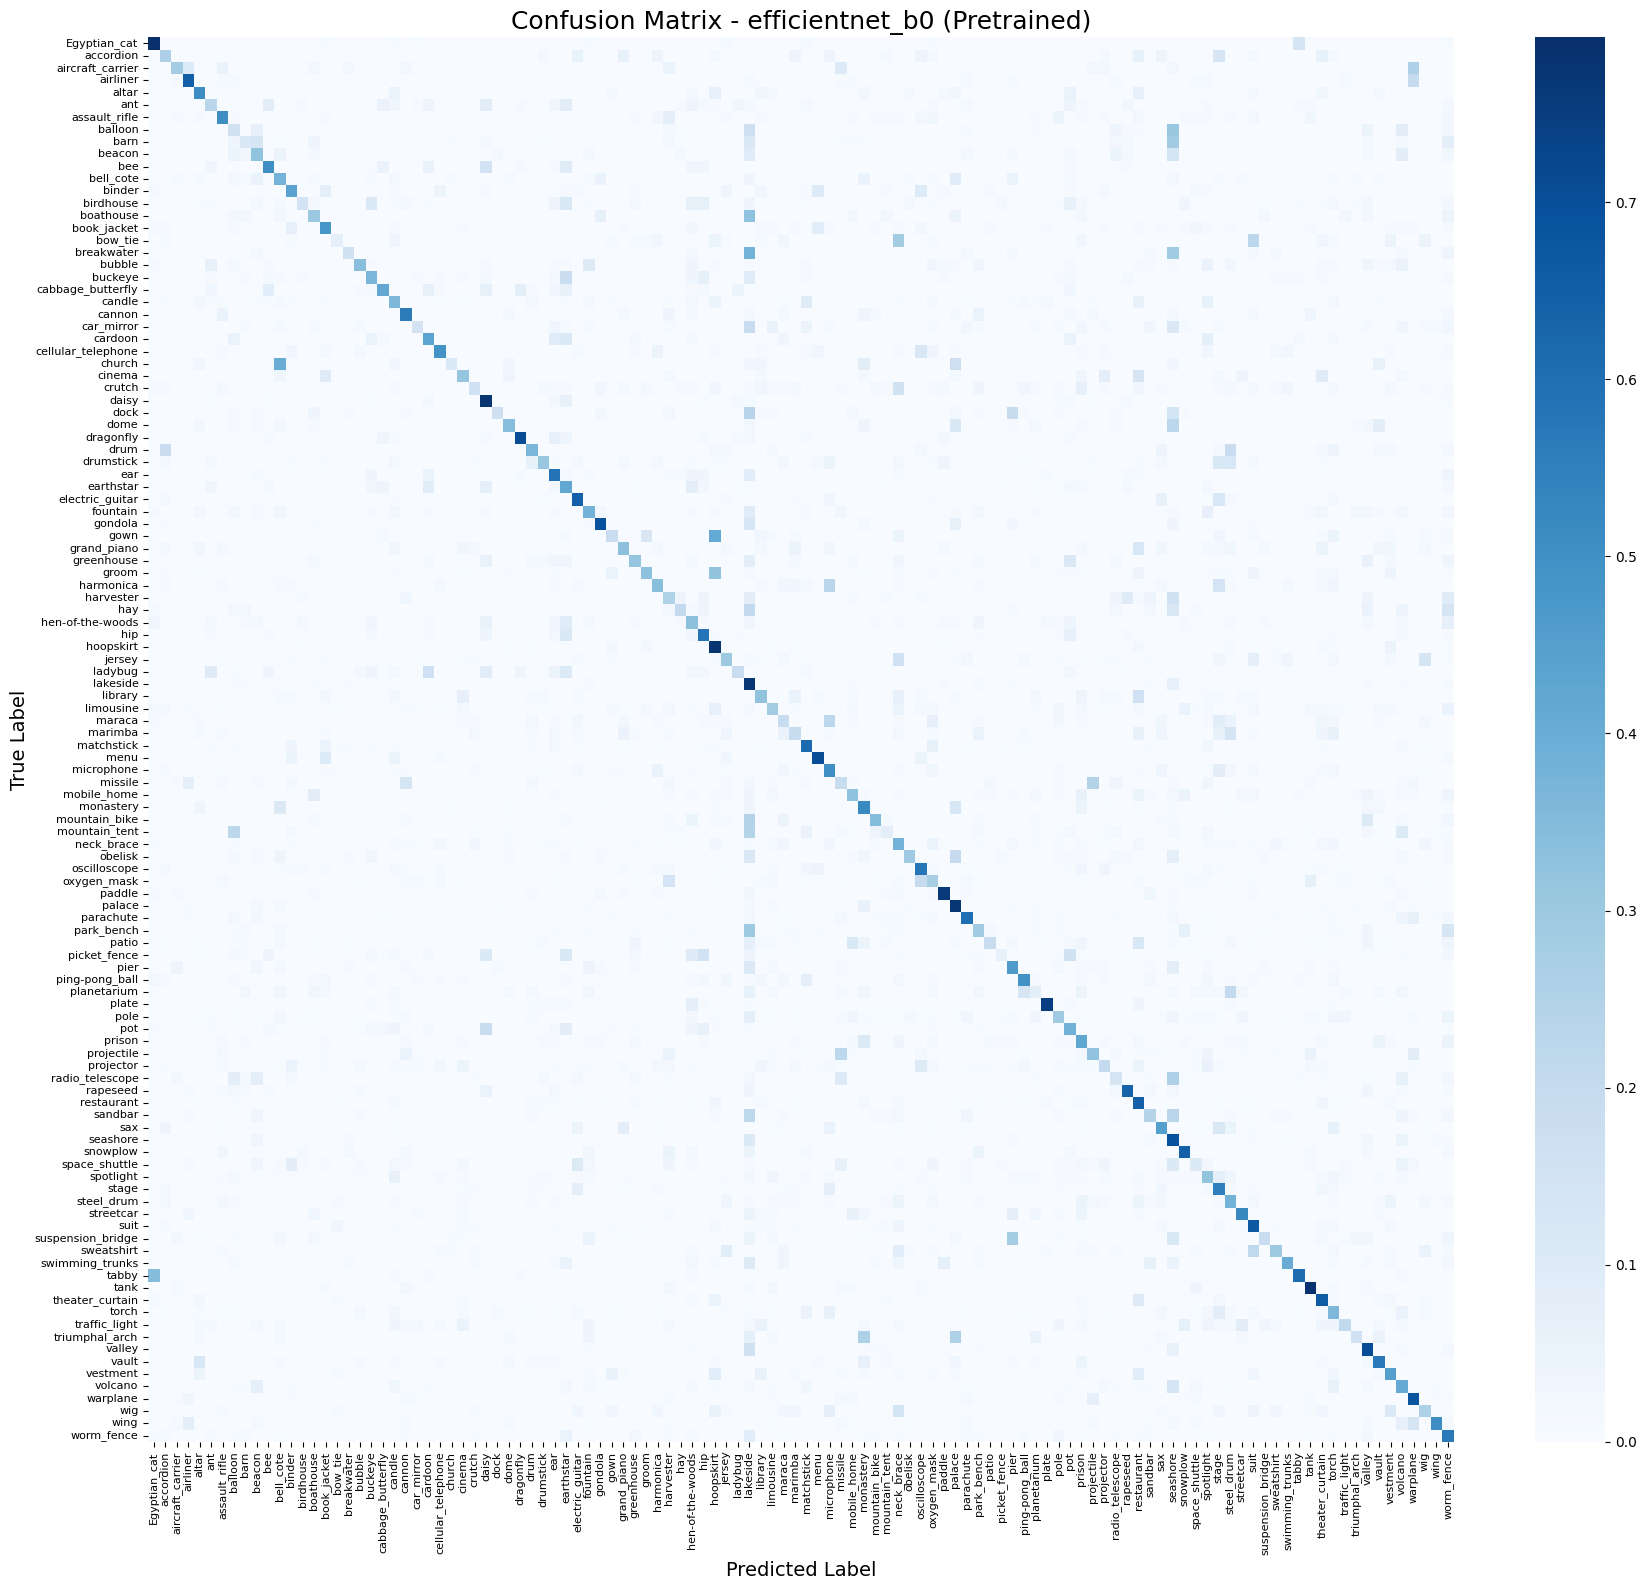
\includegraphics[width=0.8\textwidth]{images/phase01/EfficientNet-B0_normalised_conf_mat.png}
          \caption{EfficientNet-B0 tanítás nélküli normalizált Confusion Mátrix}
          \label{fig:phase01_EfficientNet-B0_normalised_conf_mat}
        \end{figure}

    \section{ConvNeXt-Tiny}
        \subsubsection{ConvNeXt-Tiny tanítás nélkül teszt}
        \begin{center}
        \begin{longtable}{l c}
        \caption{ConvNeXt-Tiny tanítás nélküli vizsgálat eredményei} \label{tab:phase01_ConvNeXt-Tiny} \\
        \toprule
        \textbf{Metrika} & \textbf{Érték} \\
        \midrule
        \endfirsthead
        \toprule
        \textbf{Metrika} & \textbf{Érték} \\
        \midrule
        \endhead
        Top-1 Accuracy & 0.5048 \\
        Top-5 Accuracy & 0.8471 \\
        Precision & 0.4917 \\
        Recall & 0.4369 \\
        F1-score & 0.4194 \\
        Inference time & 38.40 sec \\
        \bottomrule
        \end{longtable}
        \end{center}

        \subsubsection{ConvNeXt-Tiny tanítás nélküli normalizált Confusion Mátrix}
        \begin{figure}[H]
          \centering
          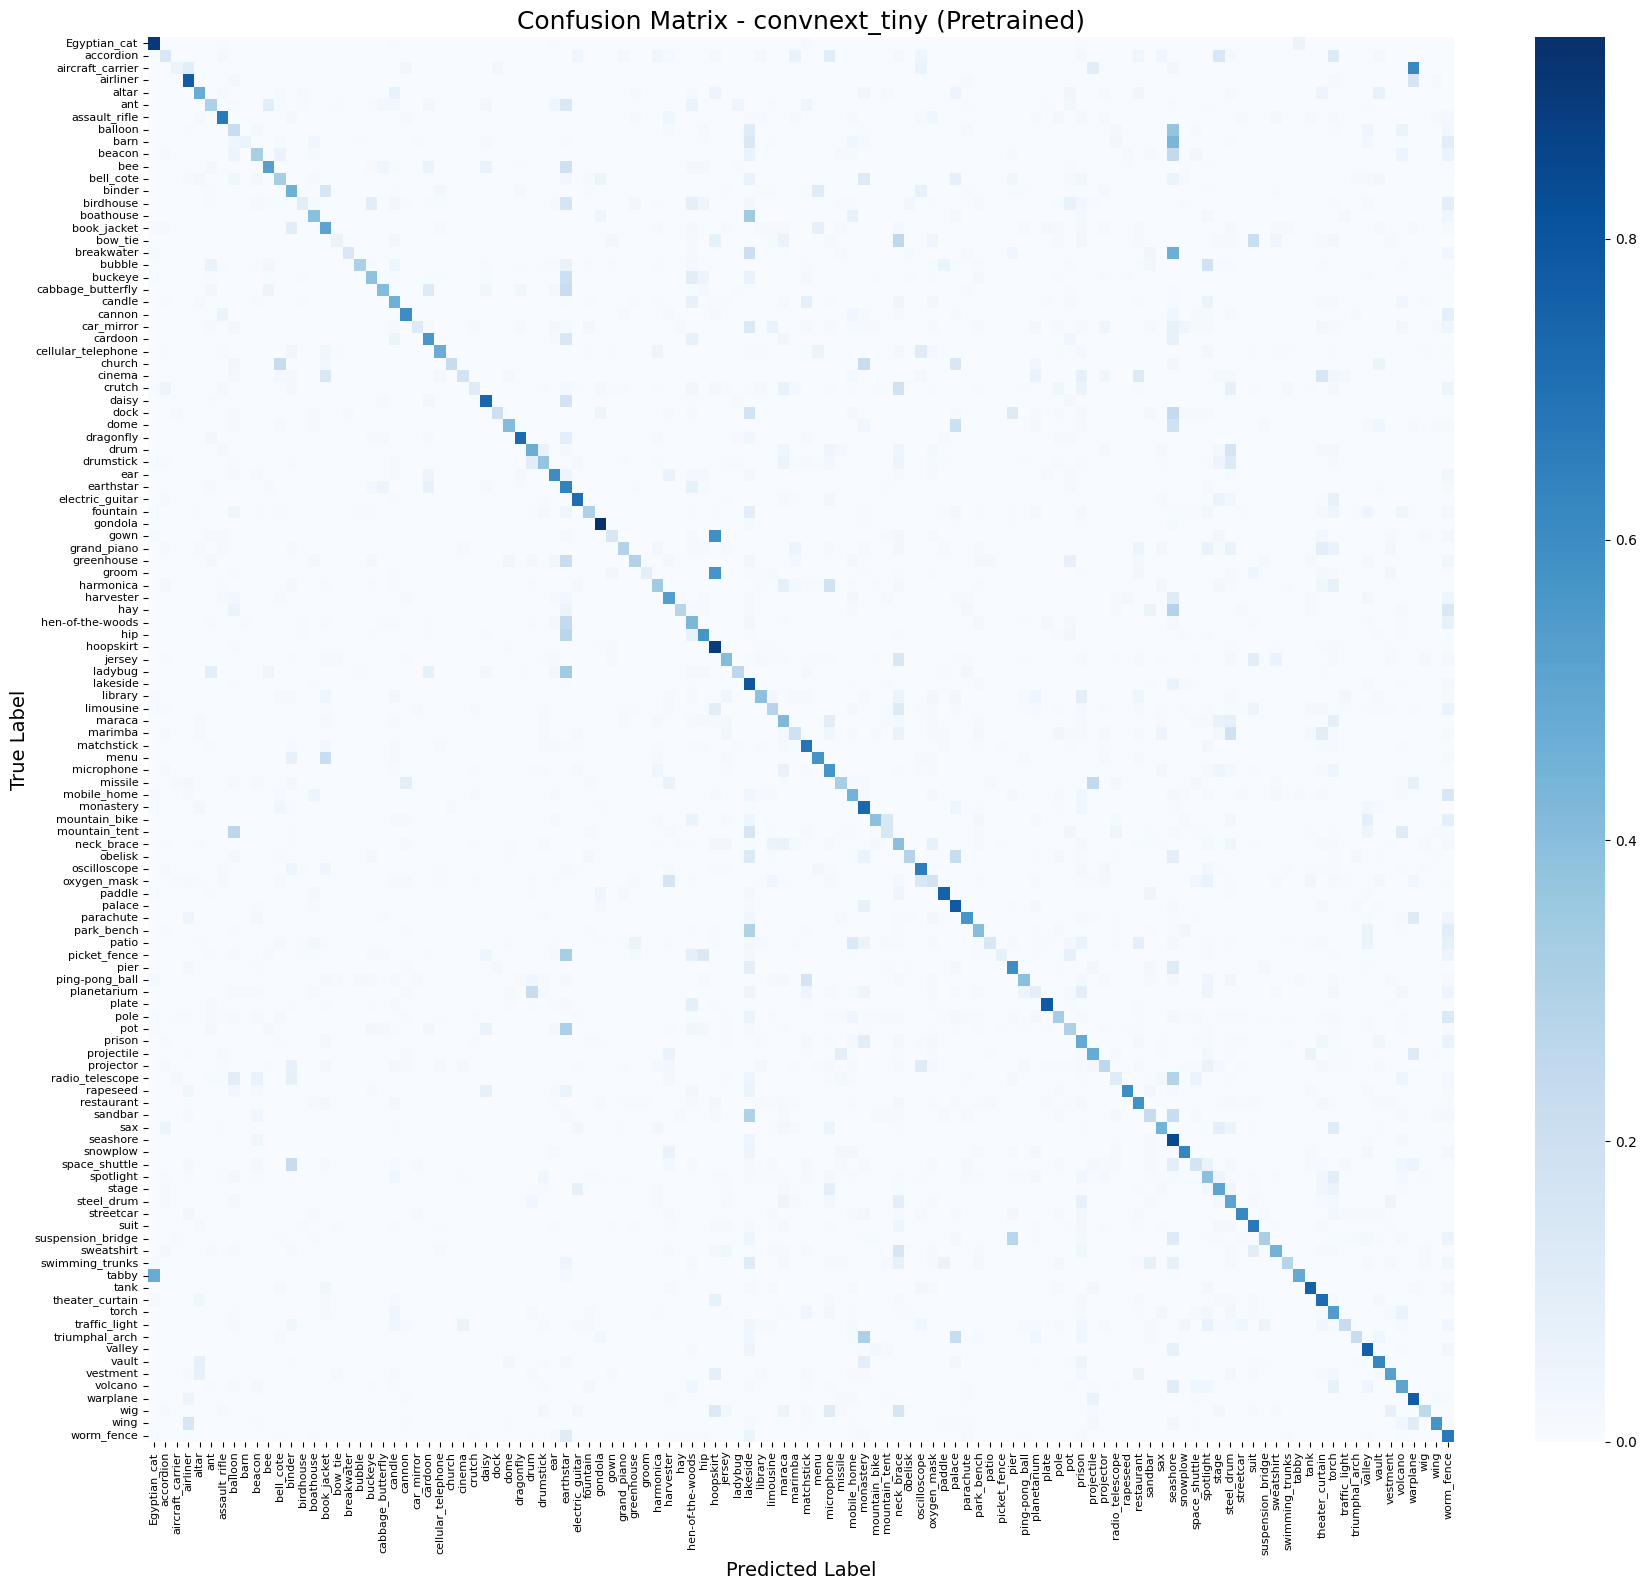
\includegraphics[width=0.8\textwidth]{images/phase01/ConvNeXt-Tiny_normalised_conf_mat.png}
          \caption{ConvNeXt-Tiny tanítás nélküli normalizált Confusion Mátrix}
          \label{fig:phase01_ConvNeXt-Tiny_normalised_conf_mat}
        \end{figure}

    \section{ViT-B/16}
        \subsubsection{ViT-B-16 tanítás nélkül teszt}
        \begin{center}
        \begin{longtable}{l c}
        \caption{ViT-B-16 tanítás nélküli vizsgálat eredményei} \label{tab:phase01_ViT-B-16} \\
        \toprule
        \textbf{Metrika} & \textbf{Érték} \\
        \midrule
        \endfirsthead
        \toprule
        \textbf{Metrika} & \textbf{Érték} \\
        \midrule
        \endhead
        Top-1 Accuracy & 0.5308 \\
        Top-5 Accuracy & 0.8582 \\
        Precision & 0.4629 \\
        Recall & 0.4419 \\
        F1-score & 0.4307 \\
        Inference time & 92.13 sec \\
        \bottomrule
        \end{longtable}
        \end{center}

        \subsubsection{ViT-B-16 tanítás nélküli normalizált Confusion Mátrix}
        \begin{figure}[H]
            \centering
            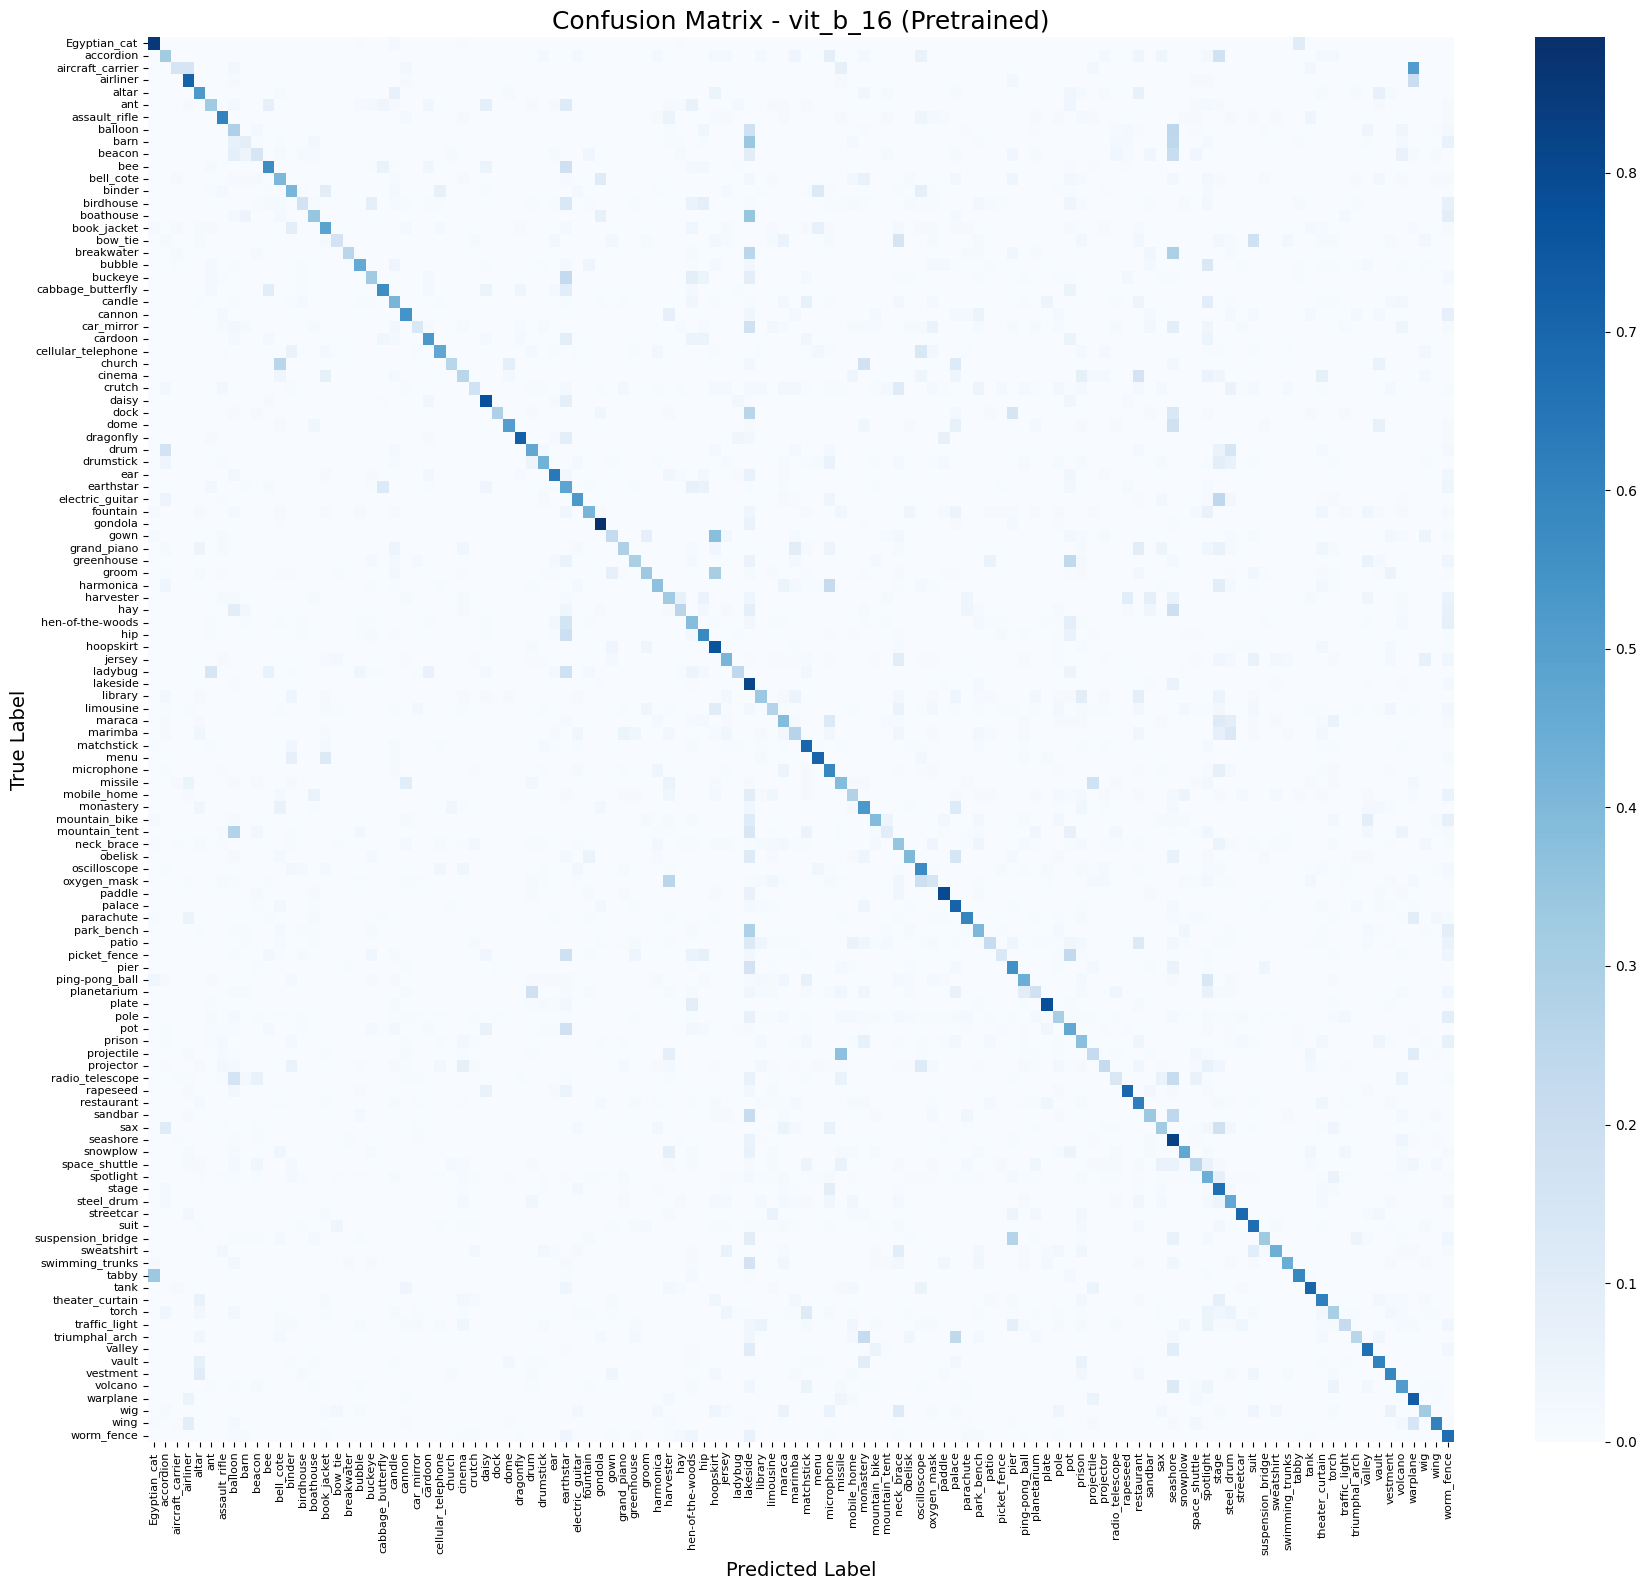
\includegraphics[width=0.8\textwidth]{images/phase01/ViT-B-16_normalised_conf_mat.png}
            \caption{ViT-B-16 tanítás nélküli normalizált Confusion Mátrix}
            \label{fig:phase01_ViT-B-16_normalised_conf_mat}
        \end{figure}

    \section{Inception-v3}
        \subsubsection{Inception-v3 tanítás nélkül teszt}
        \begin{center}
        \begin{longtable}{l c}
        \caption{Inception-v3 tanítás nélküli vizsgálat eredményei} \label{tab:phase01_Inception-v3} \\
        \toprule
        \textbf{Metrika} & \textbf{Érték} \\
        \midrule
        \endfirsthead
        \toprule
        \textbf{Metrika} & \textbf{Érték} \\
        \midrule
        \endhead
        Top-1 Accuracy & 0.4763 \\
        Top-5 Accuracy & 0.8008 \\
        Precision & 0.3833 \\
        Recall & 0.3896 \\
        F1-score & 0.3683 \\
        Inference time & 38.06 sec \\
        \bottomrule
        \end{longtable}
        \end{center}

        \subsubsection{Inception-v3 tanítás nélküli normalizált Confusion Mátrix}
        \begin{figure}[H]
          \centering
          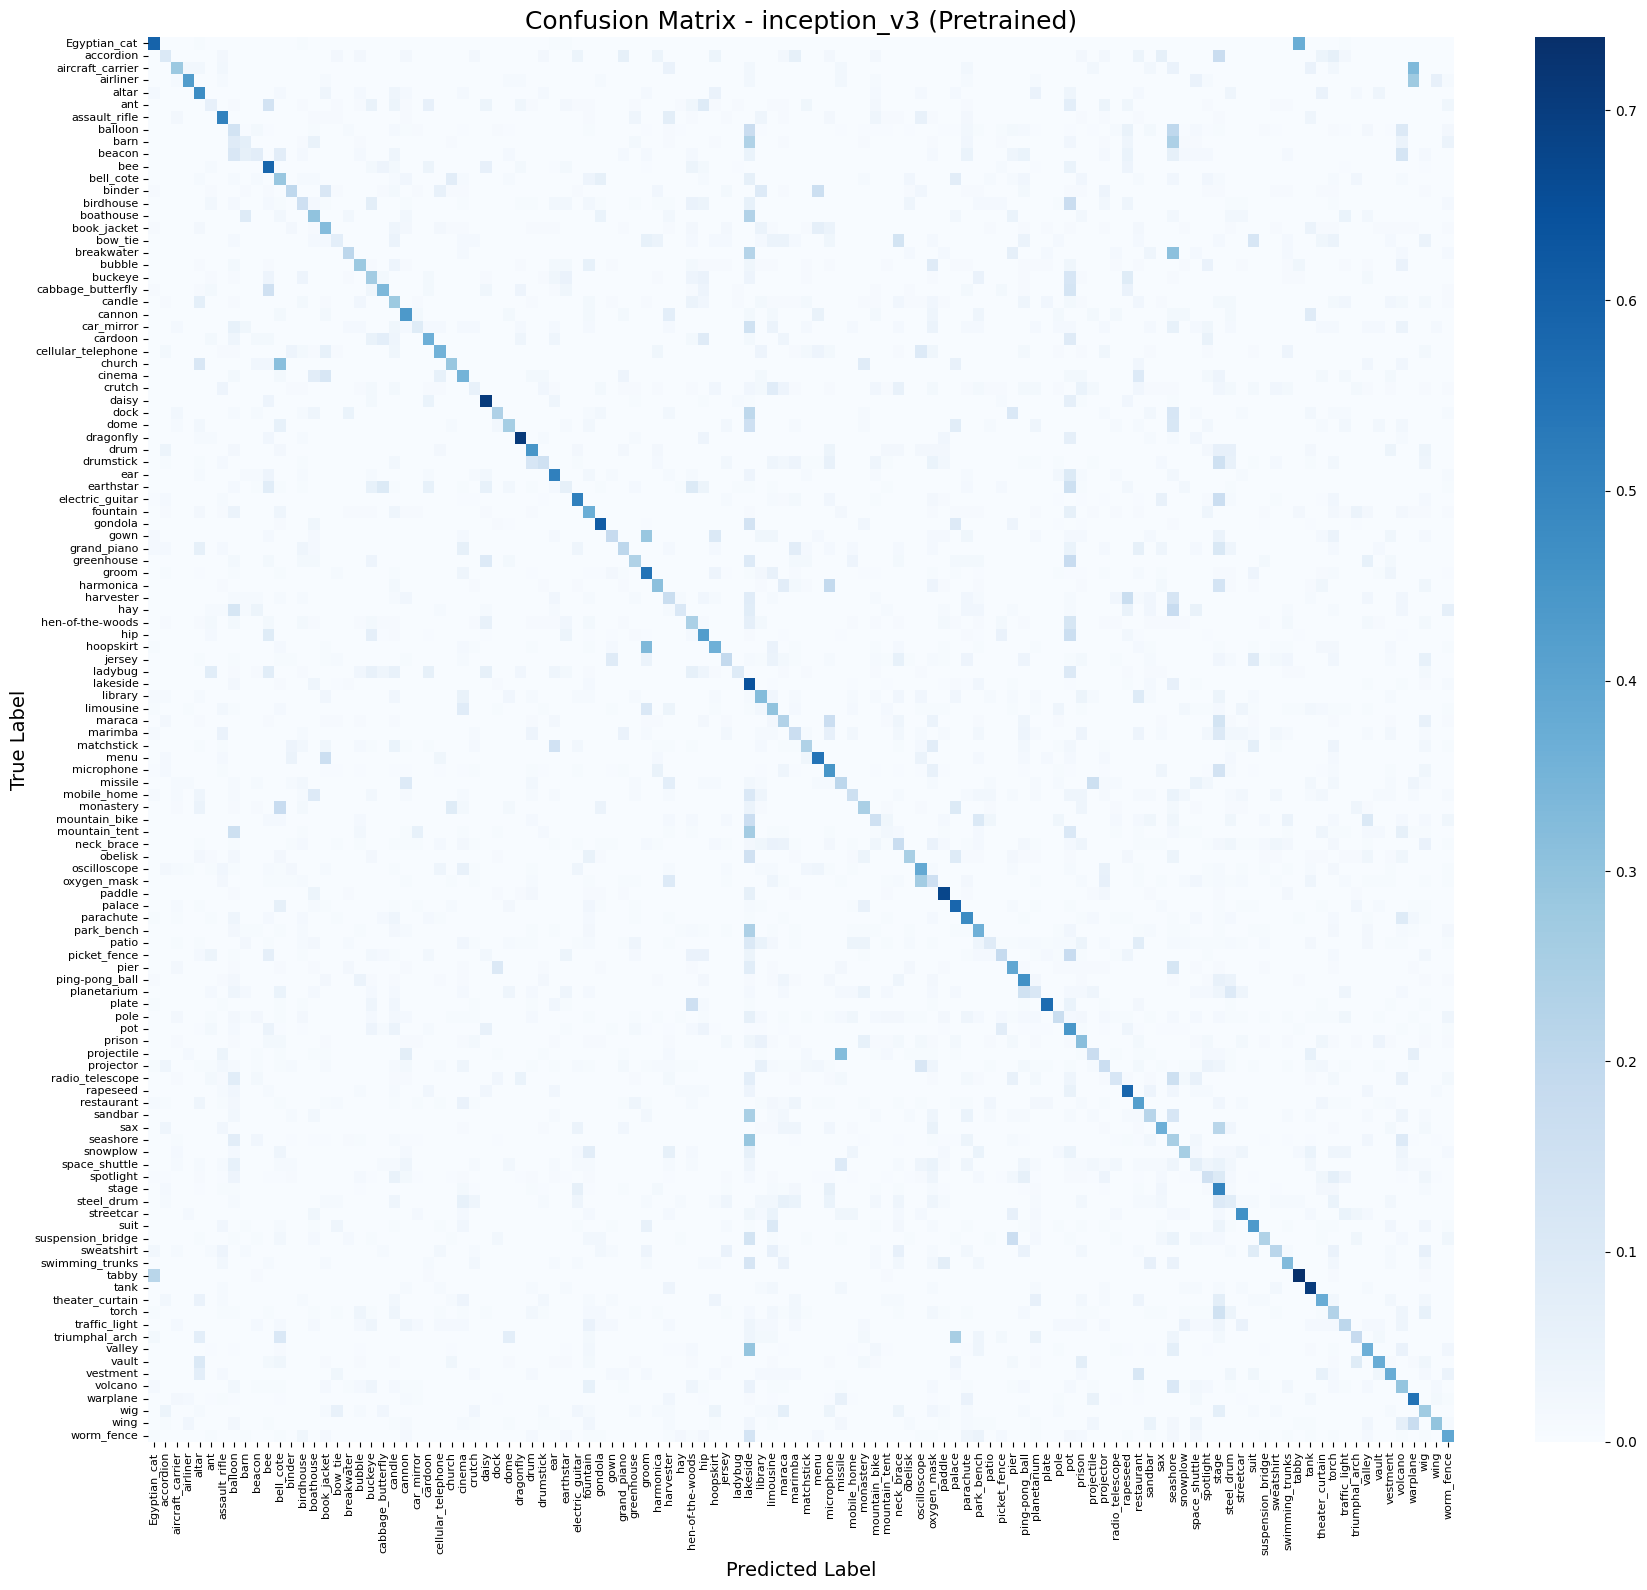
\includegraphics[width=0.8\textwidth]{images/phase01/Inception-v3_normalised_conf_mat.png}
          \caption{Inception-v3 tanítás nélküli normalizált Confusion Mátrix}
          \label{fig:phase01_Inception-v3_normalised_conf_mat}
        \end{figure}

    \section{NASNet}
        \subsubsection{NASNet tanítás nélkül teszt}
        \begin{center}
        \begin{longtable}{l c}
        \caption{NASNet tanítás nélküli vizsgálat eredményei} \label{tab:phase01_NASNet} \\
        \toprule
        \textbf{Metrika} & \textbf{Érték} \\
        \midrule
        \endfirsthead
        \toprule
        \textbf{Metrika} & \textbf{Érték} \\
        \midrule
        \endhead
        Top-1 Accuracy & 0.2820 \\
        Top-5 Accuracy & 0.5408 \\
        Precision & 0.3204 \\
        Recall & 0.2799 \\
        F1-score & 0.2696 \\
        Inference time & 275.30 sec \\
        \bottomrule
        \end{longtable}
        \end{center}

        \subsubsection{NASNet tanítás nélküli normalizált Confusion Mátrix}
        \begin{figure}[H]
          \centering
          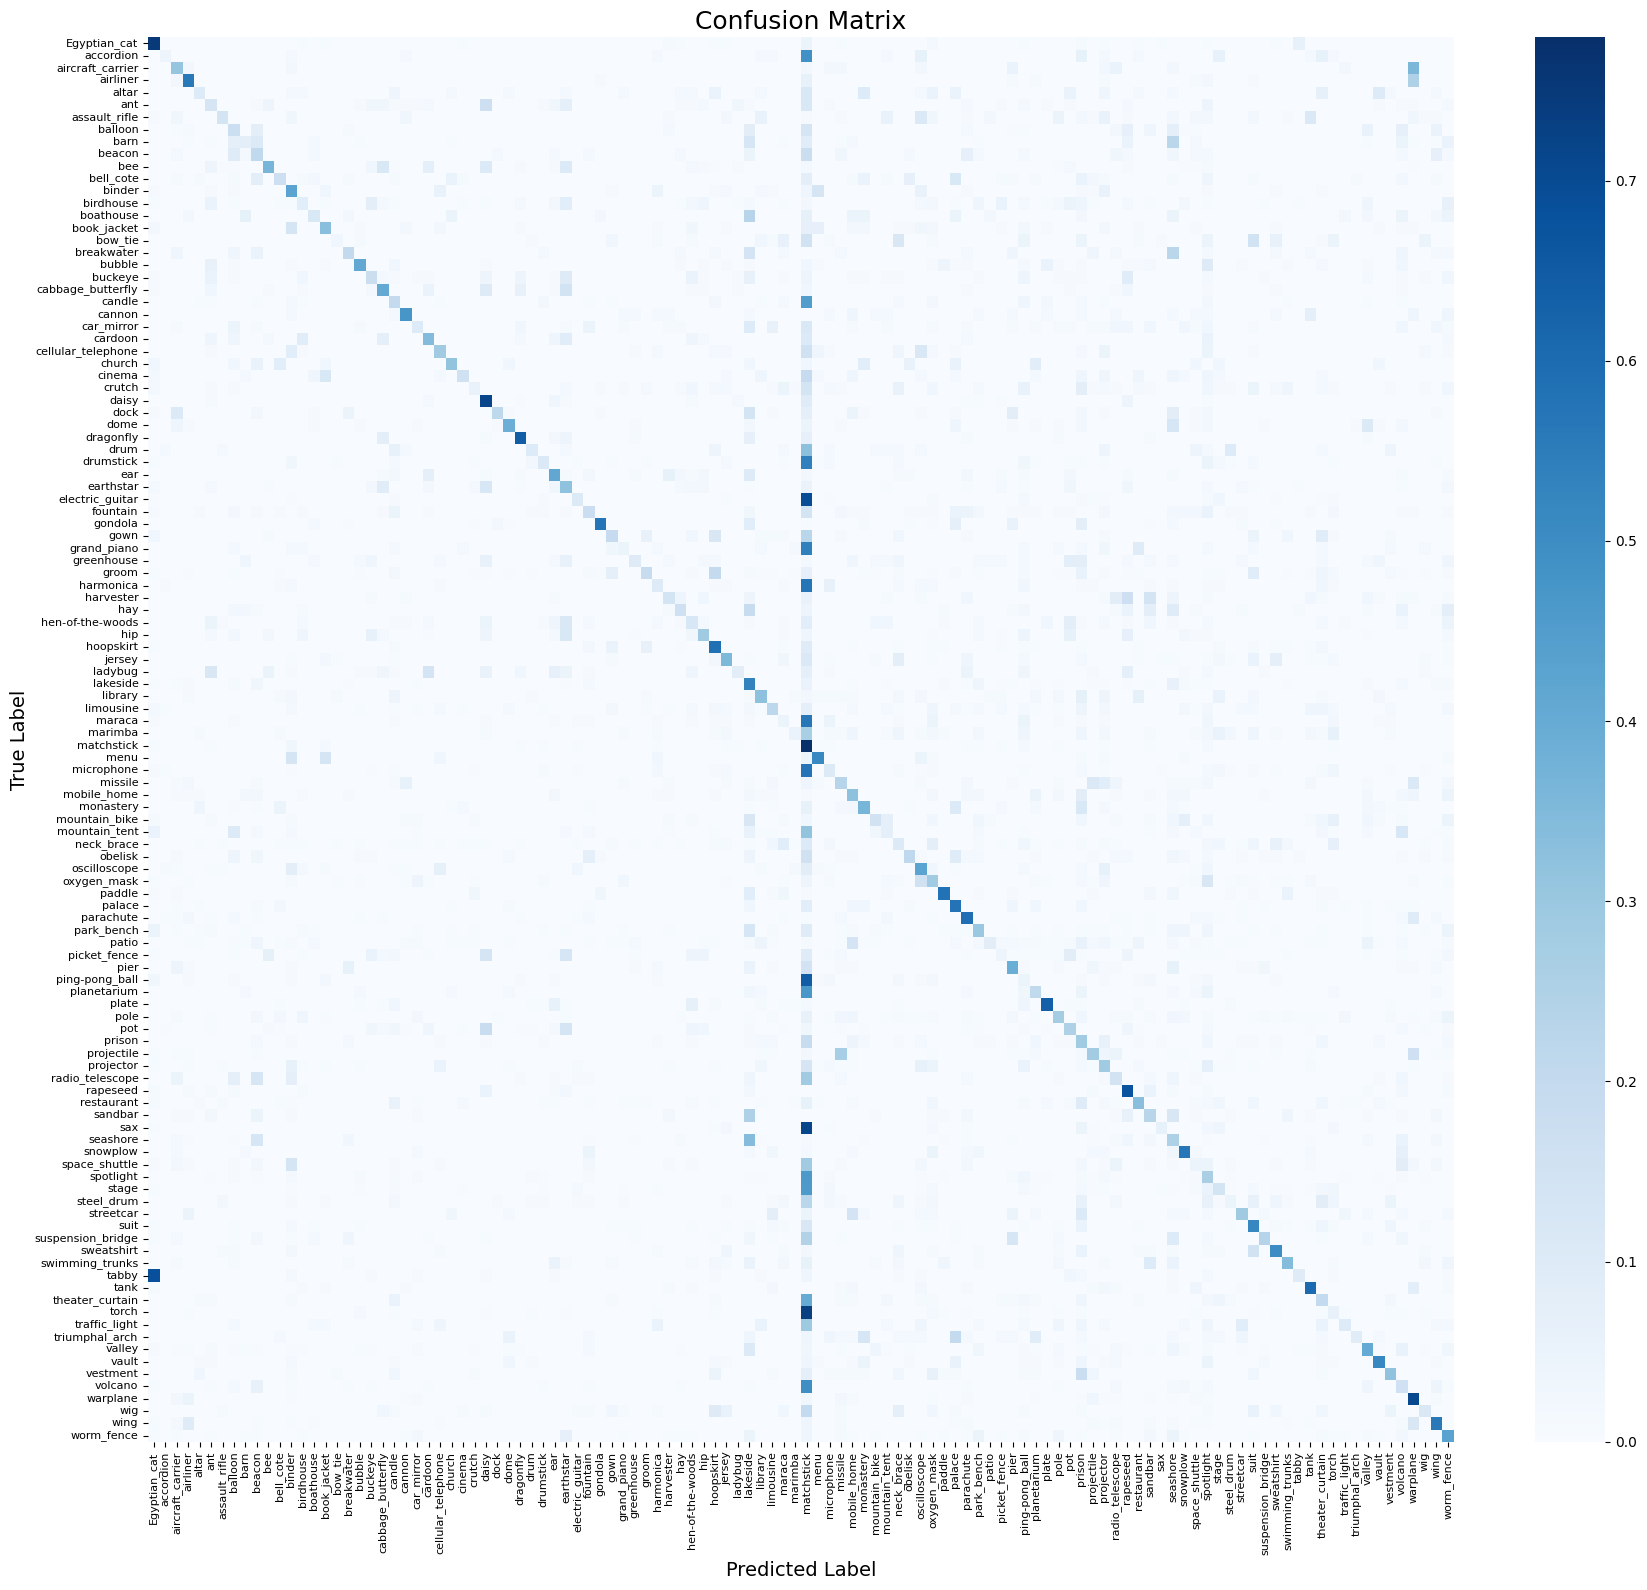
\includegraphics[width=0.8\textwidth]{images/phase01/NASNet_normalised_conf_mat.png}
          \caption{NASNet tanítás nélküli normalizált Confusion Mátrix}
          \label{fig:phase01_NASNet_normalised_conf_mat}
        \end{figure}

    \section{Összefoglaló}

    Összefoglaló az első mérési fázis eredményeiről. A hét ismert modell tanítás nélküli eredeti élsúlyokkal történő vizsgálata történt meg a saját ImageNet1k osztályozású adathalmazomon ami összesen 180750 képet tartalmaz 114 imagenet osztályba sorolva ahol nincs 300 képnél kisebb kategória Train, Val, Test halmazokra osztva 80, 10, 10 arányban. Így a Test halmaz 18172 képet tartalmaz szintén 114 kategóriára osztva. Ezen történt a hét ismert modell első fázisú tesztelése saját tanítás nélküli eredeti ImageNet1k-n előtanított súlyokkal. Nézzük most ennek a vizsgáltnak az eredményeit.


\subsubsection{Összefoglaló táblázat az első fázis mért értékeiről}
    \begin{center}
        \begin{longtable}{lllllll}
        \caption{Modellek összefoglaló értékei tanítás nélkül}\label{tab:phase1_summary_table}\\
        \toprule
        Modell & Top-1 Acc. & Top-5 Acc. & Precision & Recall & F1-score & Idő(s) \\
        \midrule
        \endfirsthead
        \toprule
        Modell & Top-1 & Top-5 & Precision & Recall & F1-score & Idő(s) \\
        \midrule
        \endhead
        ConvNeXt-Tiny & 0.5048 & 0.8471 & 0.4917 & 0.4369 & 0.4194 & 38.40 \\
        ViT-B/16 & 0.5308 & 0.8582 & 0.4629 & 0.4419 & 0.4307 & 92.13 \\
        EfficientNet-B0 & 0.4802 & 0.8217 & 0.4137 & 0.4039 & 0.3829 & 28.89 \\
        ResNet50 & 0.4698 & 0.7962 & 0.3934 & 0.3797 & 0.3592 & 25.21 \\
        DenseNet121 & 0.4498 & 0.7806 & 0.3874 & 0.3611 & 0.3408 & 25.15 \\
        Inception-v3 & 0.4763 & 0.8008 & 0.3833 & 0.3896 & 0.3683 & 38.06 \\
        NASNet & 0.2820 & 0.5408 & 0.3204 & 0.2799 & 0.2696 & 275.30 \\
        \bottomrule
        \end{longtable}
        \end{center}

    \subsubsection{Top 1 és Top 5 pontosságok összehasonlítása modellenként tanítás nélkül.}
        \begin{figure}[H]
            \centering
            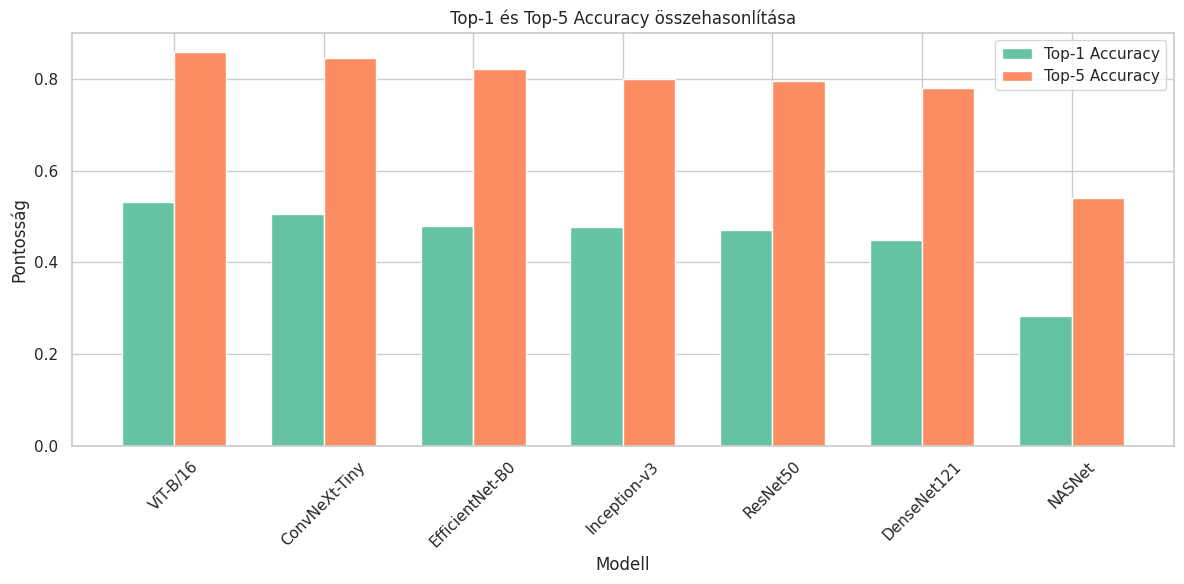
\includegraphics[width=1.0\textwidth]{images/phase01/summary01.png}
            \caption{Top 1 és Top 5 pontosságok összehasonlítása modellenként tanítás nélkül.}
            \label{fig:phase01_summary01}
        \end{figure}

    \subsubsection{Precision, Recall, F1-score összehasonlítása modellenként tanítás nélkül.}
        \begin{figure}[H]
            \centering
            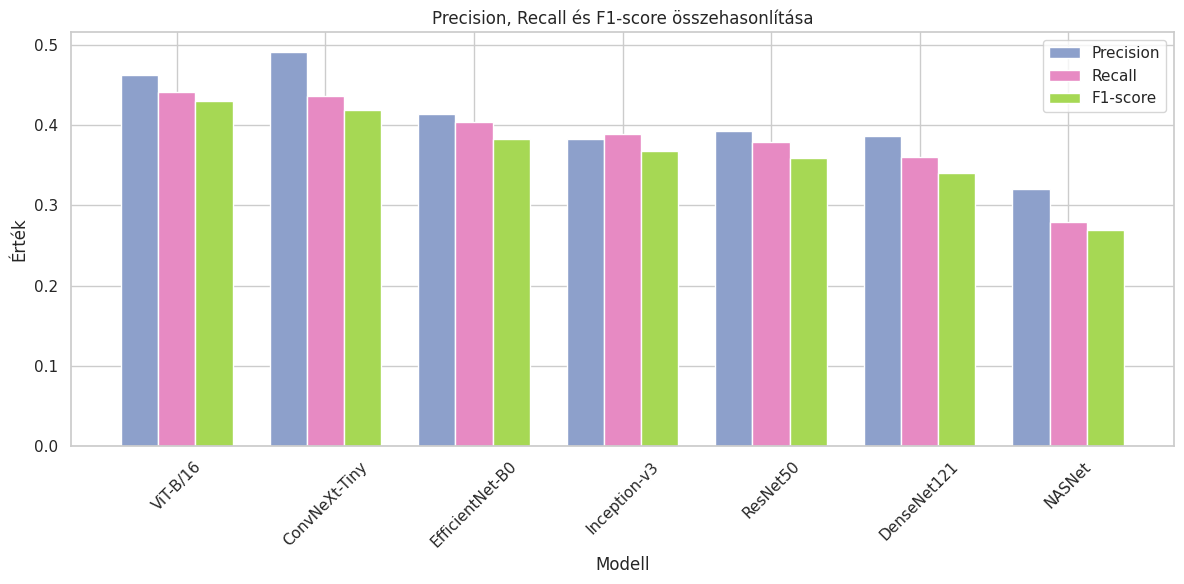
\includegraphics[width=1.0\textwidth]{images/phase01/summary02.png}
            \caption{Precision, Recall, F1-score összehasonlítása modellenként tanítás nélkül.}
            \label{fig:phase01_summary02}
        \end{figure}

    \subsubsection{Teszt lefutási idejének összehasonlítása modellenként tanítás nélkül.}
        \begin{figure}[H]
            \centering
            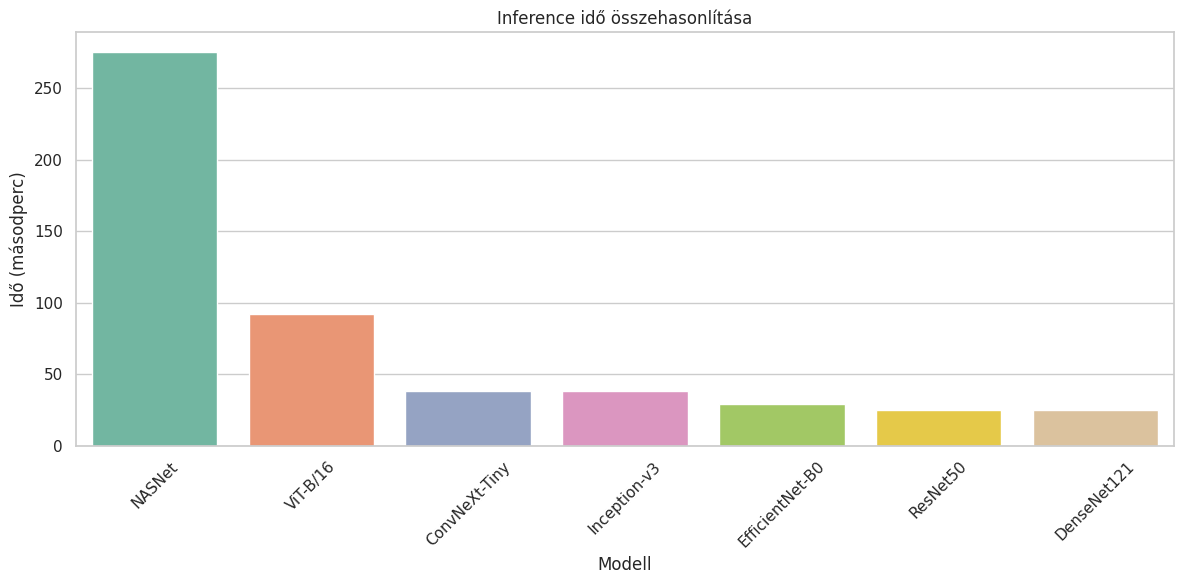
\includegraphics[width=1.0\textwidth]{images/phase01/summary03.png}
            \caption{Teszt lefutási idejének összehasonlítása modellenként tanítás nélkül.}
            \label{fig:phase01_summary03}
        \end{figure}

    \subsubsection{Az első fázis rövid szöveges értékelése}
    Az első mérési fázis során hét különböző, előre betanított modellt teszteltem a saját sb-photothemes-imagenet114 adatbázis 18000 képből álló, 114 kategóriát tartalmazó teszthalmazán. A modelleket itt az első fázisban tanítás nélkül, a gyári súlyokkal értékeltem.

    Pontosság tekintetében a ViT-B/16 modell érte el a legjobb Top-1 (53,08\%) és Top-5 (85,82\%) pontosságot, szorosan követi a ConvNeXt-Tiny és az EfficientNet-B0. Ezek az eredmények azt mutatják, hogy a transformer-alapú és modern CNN architektúrák jobban teljesítenek a hagyományosabb modelleknél, mint például a ResNet50 vagy a DenseNet121. A NASNet jelentősen alacsonyabb pontosságot ért el, ami arra utalhat, hogy nem optimalizált az adott teszthalmazra.

    Precision, Recall és F1-score mutatók alapján a ViT-B/16 és a ConvNeXt-Tiny modellek kiemelkednek, ami megerősíti a pontossági eredményeket. Ezek a modellek nemcsak pontosak, hanem megbízhatóak is a kategóriák felismerésében.

    Inference idő szempontjából a DenseNet121 és a ResNet50 modellek a leggyorsabbak (~25 másodperc), míg a NASNet jelentősen lassabb (275,30 másodperc), ami korlátozhatja a gyakorlati alkalmazhatóságát, különösen valós idejű rendszerekben.

    Összegzésként, a ViT-B/16 és a ConvNeXt-Tiny modellek kínálják a legjobb kompromisszumot a pontosság és a teljesítmény között, bár a ViT-B/16 jelentősen hosszabb inference idővel rendelkezik. A DenseNet121 és a ResNet50 gyorsabbak, de alacsonyabb pontosságot nyújtanak. A NASNet alacsony pontossága és hosszú inference ideje miatt kevésbé ajánlott az adott feladatra.

\chapter{II. Fázis: Teljes tanítás}
    Ebben a fázisban minden modellt teljesen betanítottam a teljes 144600 képet tartalmazó tanítóhalmazon. A tanítás során 10 epochon keresztül zajlott a modell optimalizálása, kivéve a NASNet modellt, ahol a számítási kapacitás korlátai miatt csak 2 epochig tartott a tréning.
    
    \textbf{Cél:} A modellek maximális, hosszú távú tanulási potenciáljának feltérképezése az egész adathalmazon.

    \section{ResNet50}
        \subsubsection{ResNet50 teljes tanítás folyamata}
        \begin{figure}[H]
        \centering
        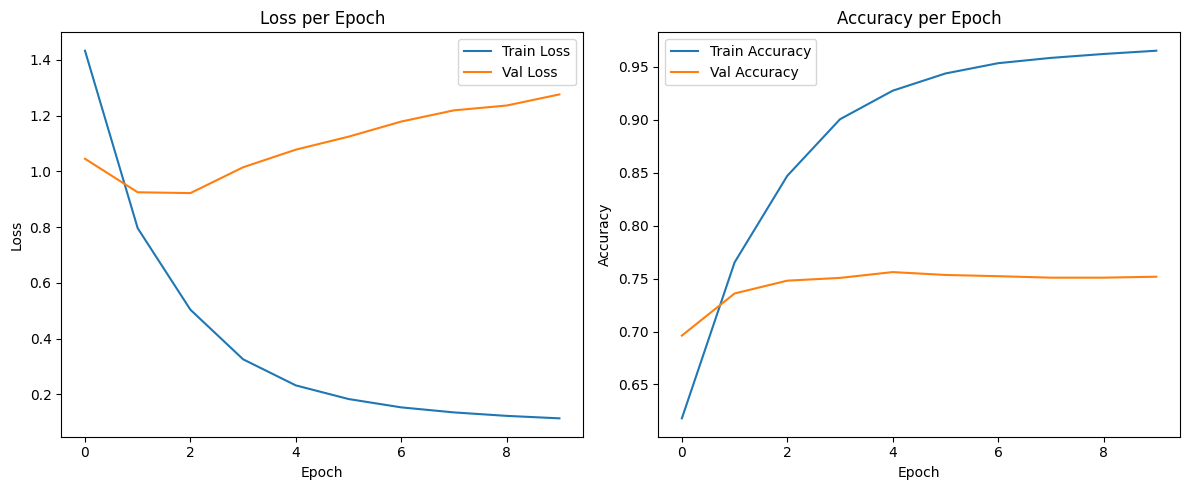
\includegraphics[width=1.0\textwidth]{images/phase02/ResNet50_learning_curve.png}
        \caption{ResNet50 teljes tanítás utáni sima Confusion Mátrix}
        \label{fig:phase02_ResNet50_learning_curves}
        \end{figure}
  
        \subsubsection{ResNet50 teljes tanítás utáni eredményei}
        \begin{center}
        \begin{longtable}{l c}
        \caption{ResNet50 teljes tanítás utáni vizsgálati eredményei} \label{tab:phase02_ResNet50} \\
        \toprule
        \textbf{Metrika} & \textbf{Érték} \\
        \midrule
        \endfirsthead
        \toprule
        \textbf{Metrika} & \textbf{Érték} \\
        \midrule
        \endhead
        Top-1 Accuracy & 0.7553 \\
        Top-5 Accuracy & 0.9351 \\
        Precision & 0.7110 \\
        Recall & 0.6808 \\
        F1-score & 0.6908 \\
        Inference time & 25.11 sec \\
        \bottomrule
        \end{longtable}
        \end{center}
    
        \subsubsection{ResNet50 eredményeinek összehasonlítása}
        \begin{center}
        \begin{longtable}{l c c}
        \caption{ResNet50 eredményeinek összehasonlítása} \label{tab:phase02_ResNet50_compare} \\
        \toprule
        \textbf{Metrika} & \textbf{Pretrained} & \textbf{Fine-tuned} \\
        \midrule
        \endfirsthead
        \toprule
        \textbf{Metrika} & \textbf{Pretrained} & \textbf{Fine-tuned} \\
        \midrule
        \endhead
        Top-1 Accuracy  & 0.4698 & 0.7553 \\
        Top-5 Accuracy & 0.7962 & 0.9351 \\
        Precision & 0.3934 & 0.7110 \\
        Recall & 0.3797 & 0.6808 \\
        F1-score & 0.3592 & 0.6908 \\
        Inference time & 25.21 sec & 25.11 sec \\
        \bottomrule
        \end{longtable}
        \end{center}
    
        \subsubsection{ResNet50 eredményeinek összehasonlítása}
        \begin{figure}[H]
        \centering
        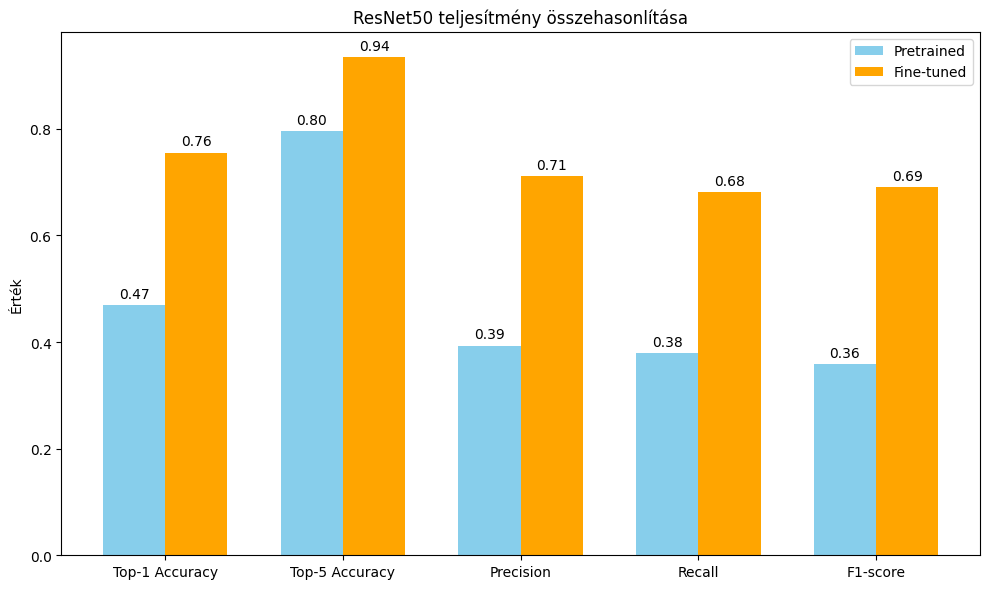
\includegraphics[width=1.0\textwidth]{images/phase02/ResNet50_compare01.png}
        \caption{ResNet50 eredményeinek összehasonlítása}
        \label{fig:ResNet50_compare01}
        \end{figure}
    
        \subsubsection{ResNet50 eredményeinek összehasonlítása}
        \begin{figure}[H]
        \centering
        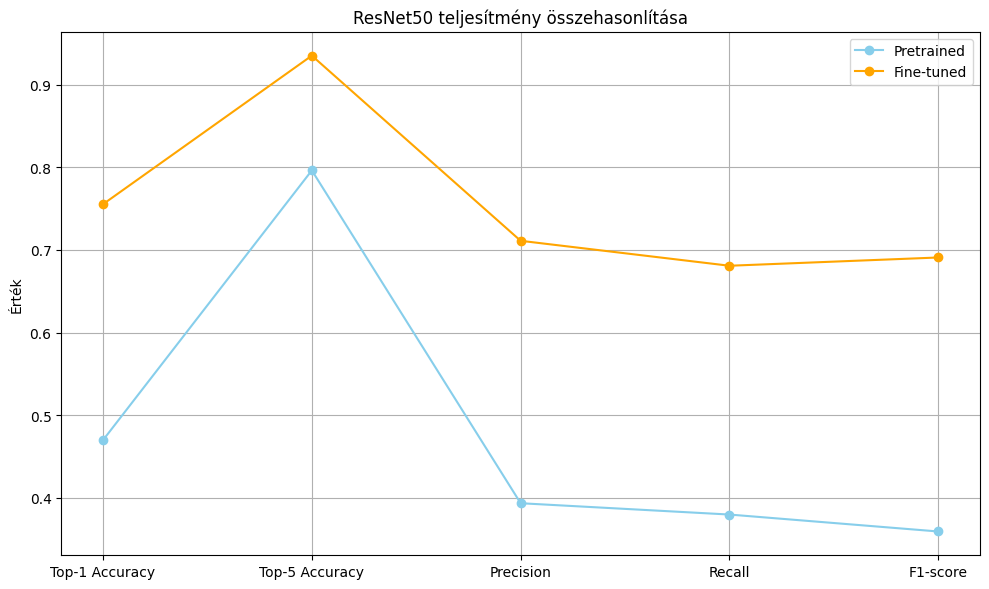
\includegraphics[width=1.0\textwidth]{images/phase02/ResNet50_compare02.png}
        \caption{ResNet50 eredményeinek összehasonlítása}
        \label{fig:ResNet50_compare02}
        \end{figure}

        \subsubsection{ResNet50 teljes tanítás utáni normalizált Confusion Mátrix}
        \begin{figure}[H]
          \centering
          
\includegraphics[width=0.8\textwidth]{images/phase02/ResNet50_normalised_conf_mat.png}
          \caption{ResNet50 teljes tanítás utáni normalizált Confusion Mátrix}
          \label{fig:phase02_ResNet50_normalised_conf_mat}
        \end{figure}
      
        \subsubsection{ResNet50 normalizált Confusion Mátrixok összehasonlítása}
        \begin{figure}[H]
          \centering
          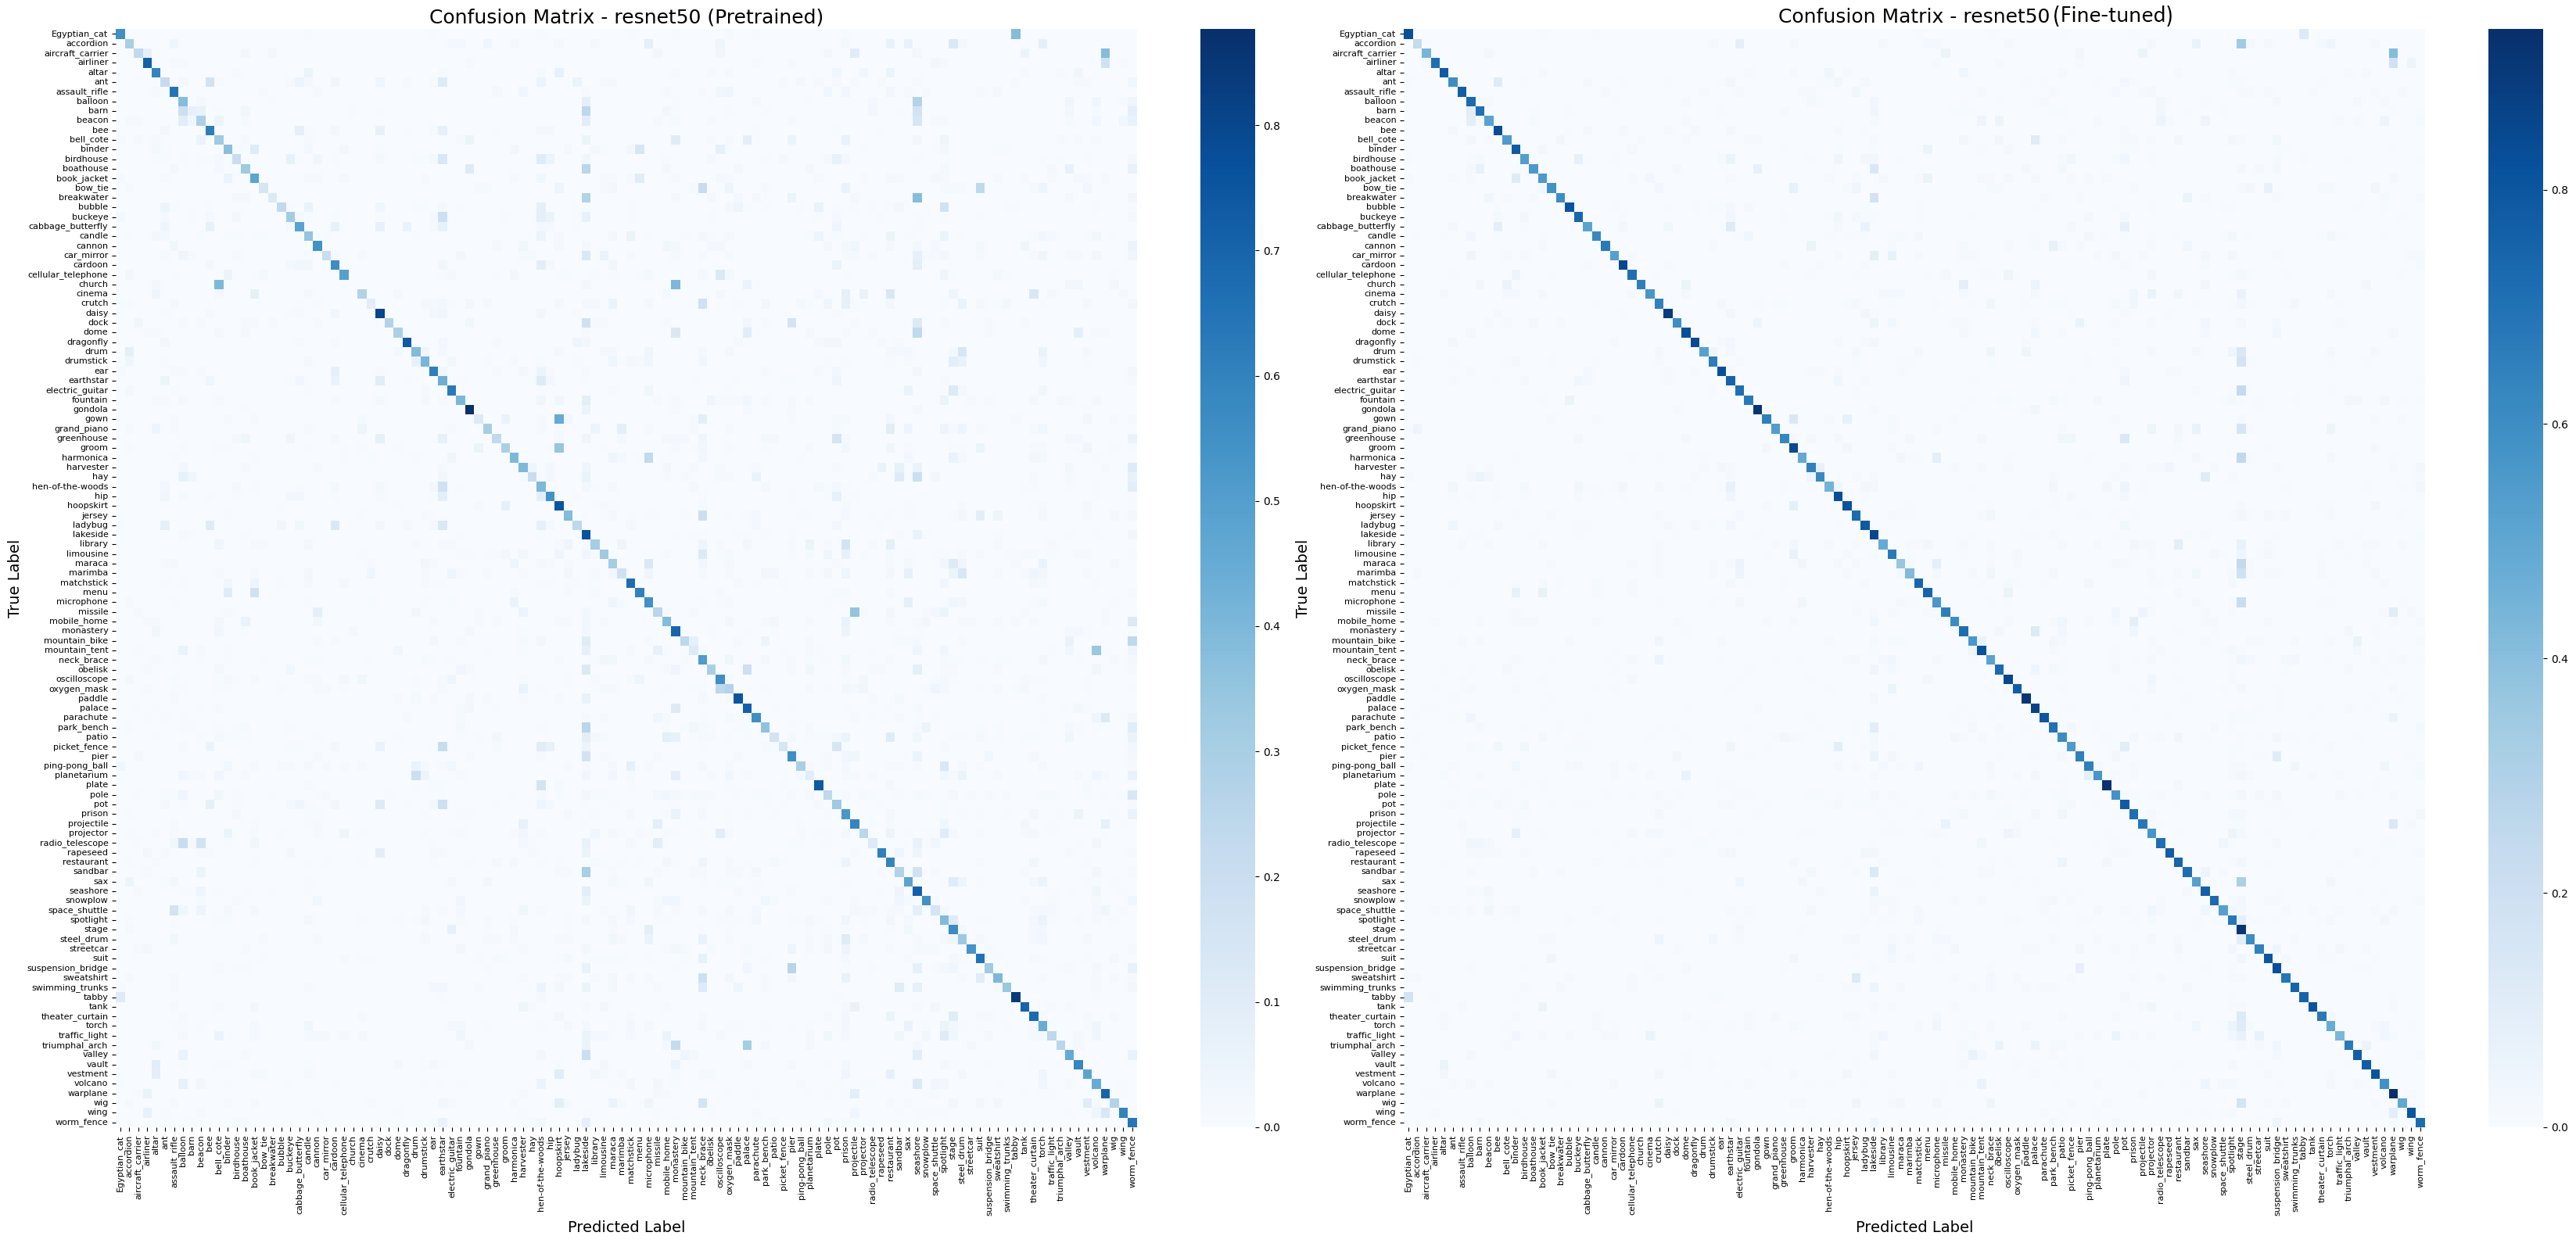
\includegraphics[width=1.0\textwidth]{images/phase02/ResNet50_normalised_conf_mat_compare.png}
          \caption{ResNet50 normalizált Confusion Mátrixok összehasonlítása}
          \label{fig:phase02_ResNet50_normalised_conf_mat_compare}
        \end{figure}

    \section{DenseNet121}
    \subsubsection{DenseNet121 teljes tanítás folyamata}
    \begin{figure}[H]
      \centering
      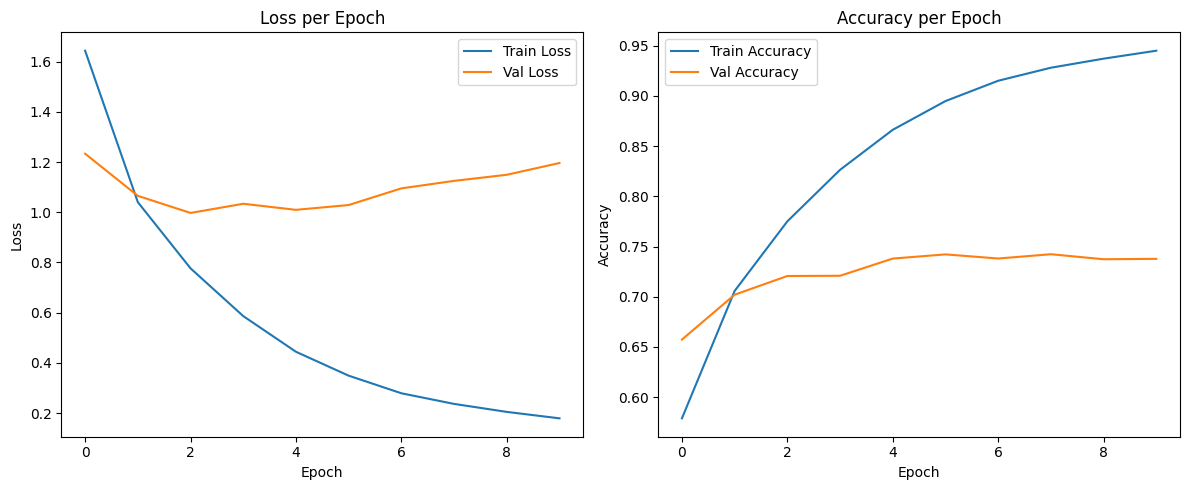
\includegraphics[width=1.0\textwidth]{images/phase02/DenseNet121_learning_curve.png}
      \caption{DenseNet121 teljes tanítás utáni sima Confusion Mátrix}
      \label{fig:phase02_DenseNet121_learning_curves}
    \end{figure}
  
  \subsubsection{DenseNet121 teljes tanítás utáni eredményei}
    \begin{center}
    \begin{longtable}{l c}
    \caption{DenseNet121 teljes tanítás utáni vizsgálati eredményei} \label{tab:phase02_DenseNet121} \\
    \toprule
    \textbf{Metrika} & \textbf{Érték} \\
    \midrule
    \endfirsthead
    \toprule
    \textbf{Metrika} & \textbf{Érték} \\
    \midrule
    \endhead
    Top-1 Accuracy & 0.7400 \\
    Top-5 Accuracy & 0.9266 \\
    Precision & 0.6811 \\
    Recall & 0.6808 \\
    F1-score & 0.6696 \\
    Inference time & 25.23 sec \\
    \bottomrule
    \end{longtable}
    \end{center}
  
  \subsubsection{DenseNet121 eredményeinek összehasonlítása}
    \begin{center}
    \begin{longtable}{l c c}
    \caption{DenseNet121 eredményeinek összehasonlítása} \label{tab:phase02_DenseNet121_compare} \\
    \toprule
    \textbf{Metrika} & \textbf{Pretrained} & \textbf{Fine-tuned} \\
    \midrule
    \endfirsthead
    \toprule
    \textbf{Metrika} & \textbf{Pretrained} & \textbf{Fine-tuned} \\
    \midrule
    \endhead
    Top-1 Accuracy  & 0.4498 & 0.7400 \\
    Top-5 Accuracy & 0.7806 & 0.9266 \\
    Precision & 0.3874 & 0.6811 \\
    Recall & 0.3611 & 0.6680 \\
    F1-score & 0.3408 & 0.6696 \\
    Inference time & 25.15 sec & 25.23 sec \\
    \bottomrule
    \end{longtable}
    \end{center}
  
  \subsubsection{DenseNet121 eredményeinek összehasonlítása}
    \begin{figure}[H]
      \centering
      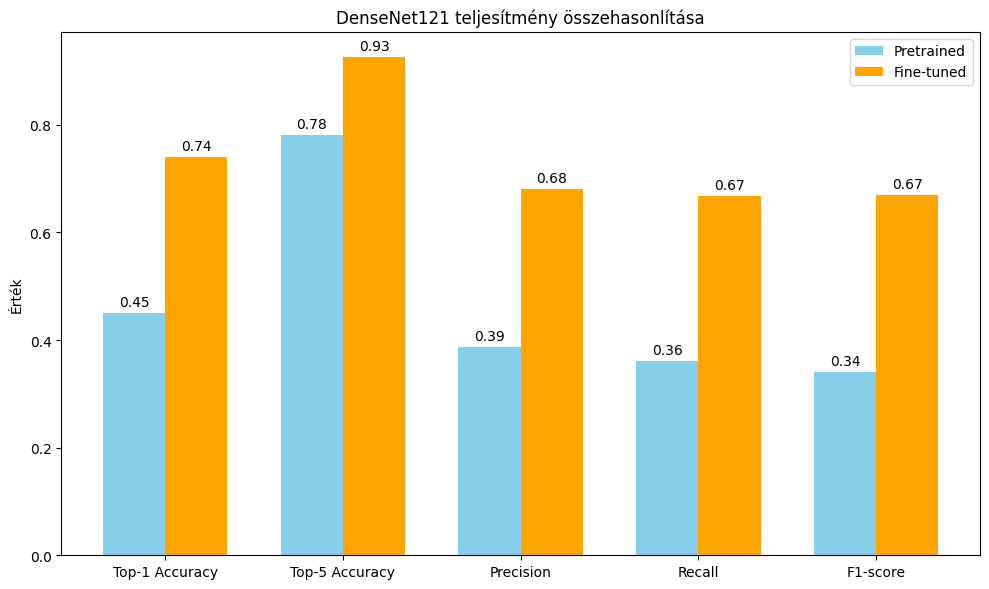
\includegraphics[width=1.0\textwidth]{images/phase02/DenseNet121_compare01.png}
      \caption{DenseNet121 eredményeinek összehasonlítása}
      \label{fig:DenseNet121_compare01}
    \end{figure}
  
  \subsubsection{DenseNet121 eredményeinek összehasonlítása}
    \begin{figure}[H]
      \centering
      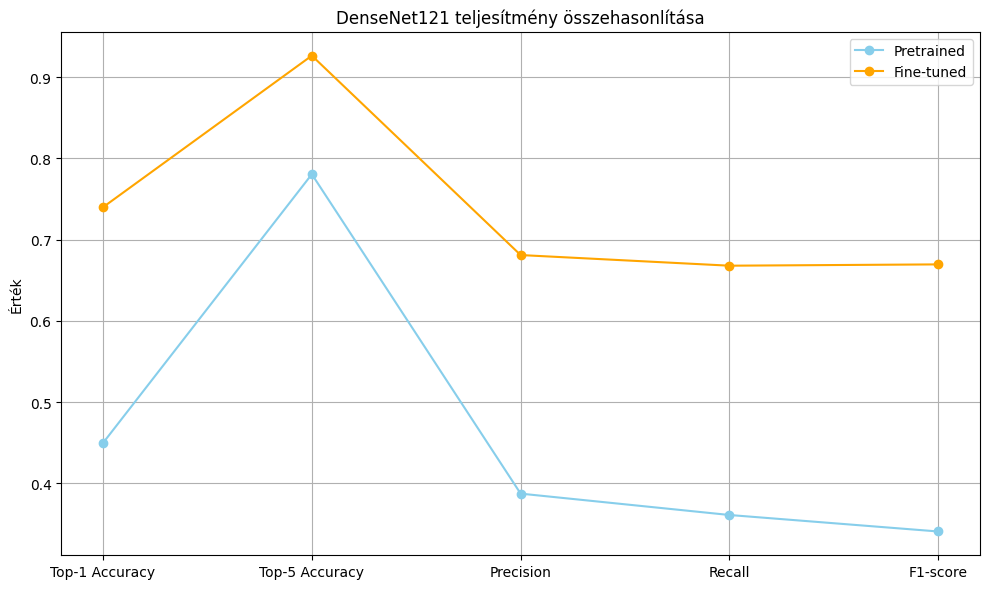
\includegraphics[width=1.0\textwidth]{images/phase02/DenseNet121_compare02.png}
      \caption{DenseNet121 eredményeinek összehasonlítása}
      \label{fig:DenseNet121_compare02}
    \end{figure}

    \subsubsection{DenseNet121 teljes tanítás utáni normalizált Confusion Mátrix}
    \begin{figure}[H]
      \centering
      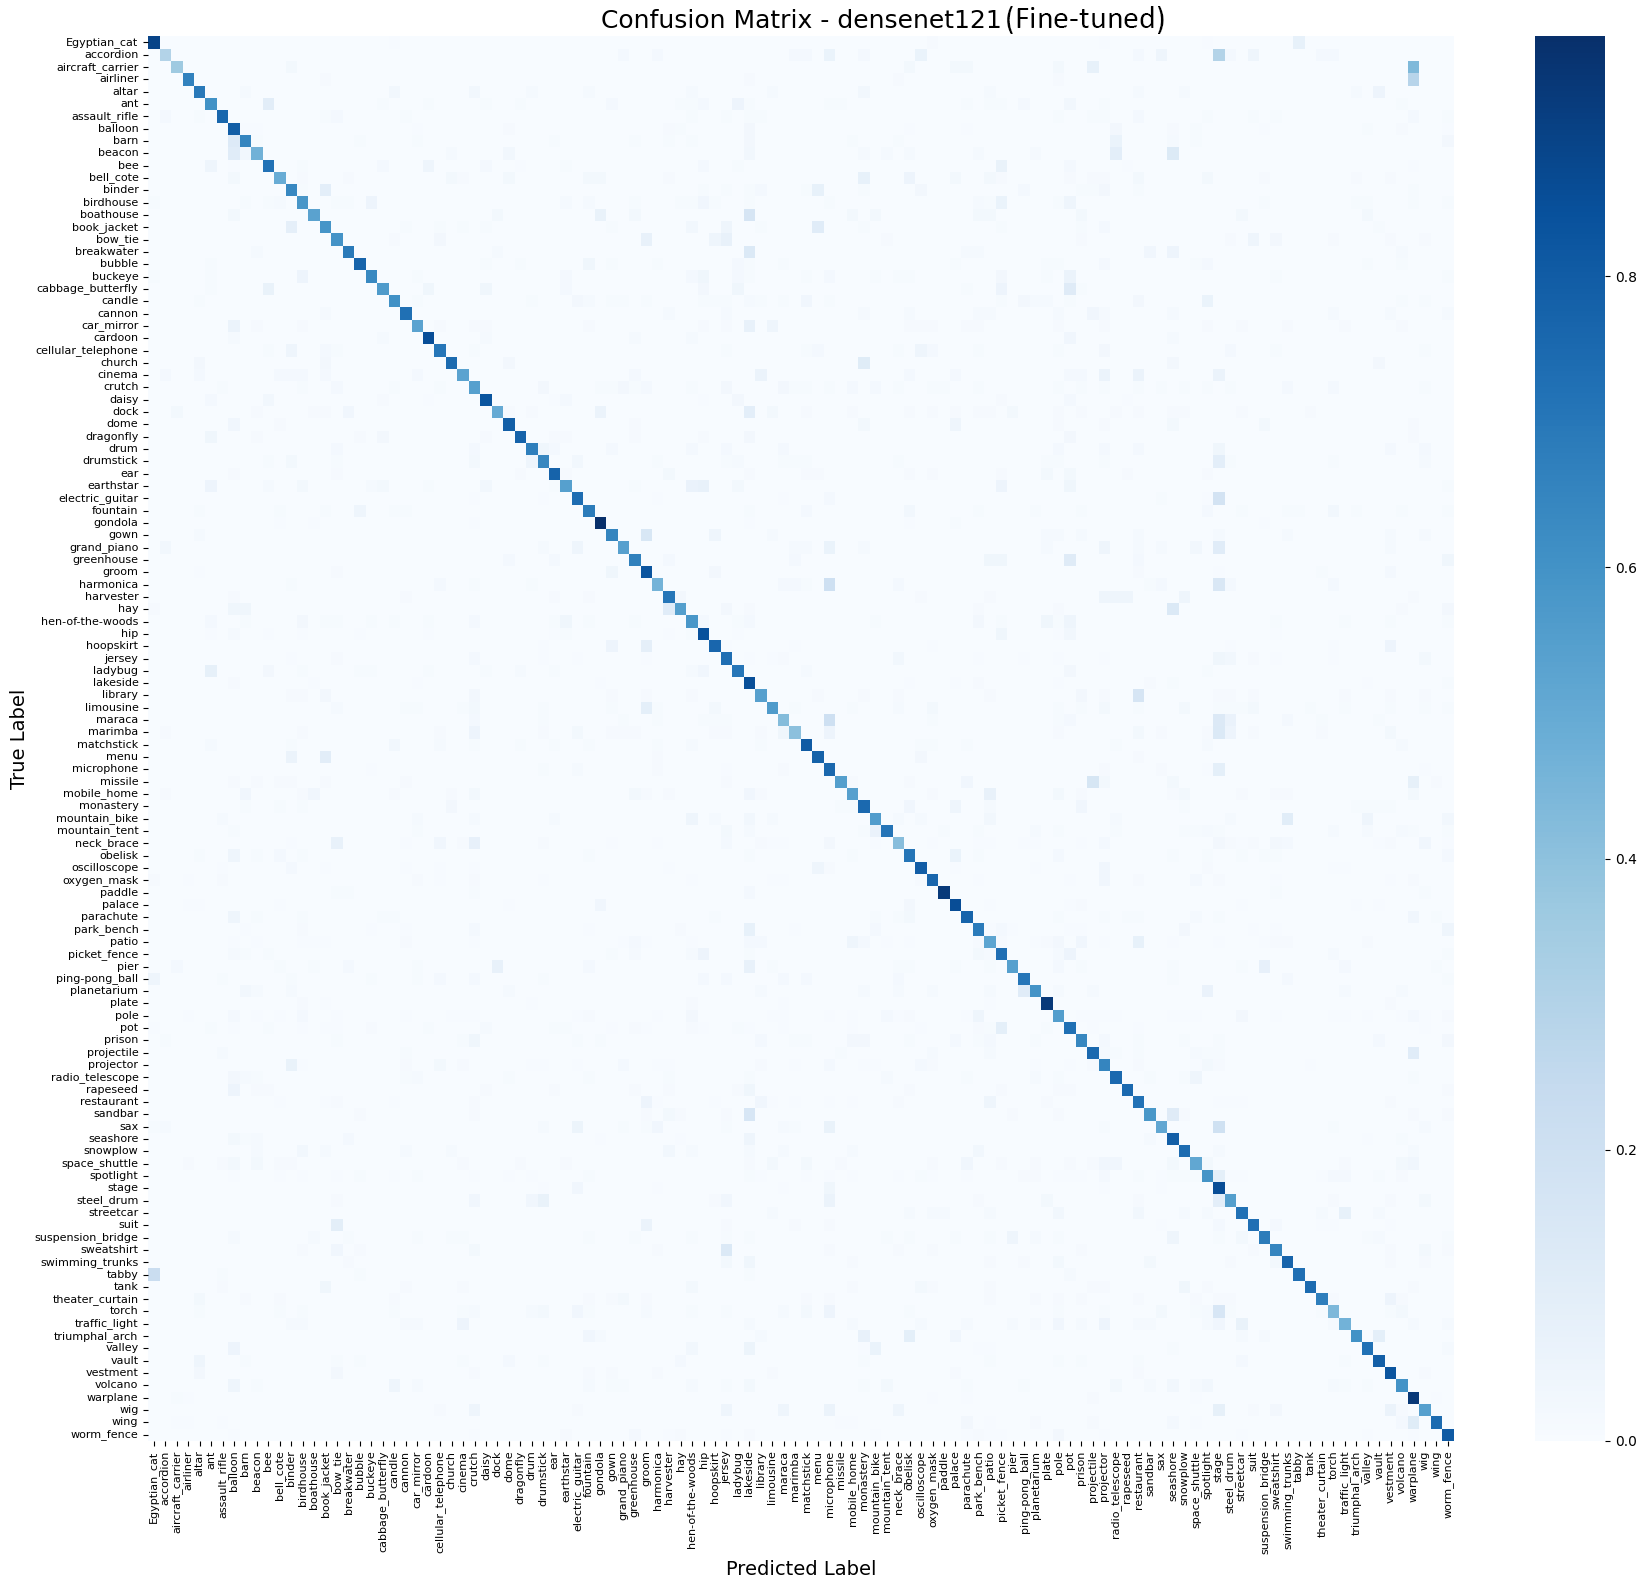
\includegraphics[width=0.8\textwidth]{images/phase02/phase02_DenseNet121_normalised_conf_mat.png}
      \caption{DenseNet121 teljes tanítás utáni normalizált Confusion Mátrix}
      \label{fig:phase02_DenseNet121_normalised_conf_mat}
    \end{figure}
  
    \subsubsection{DenseNet121 normalizált Confusion Mátrixok összehasonlítása}
    \begin{figure}[H]
      \centering
      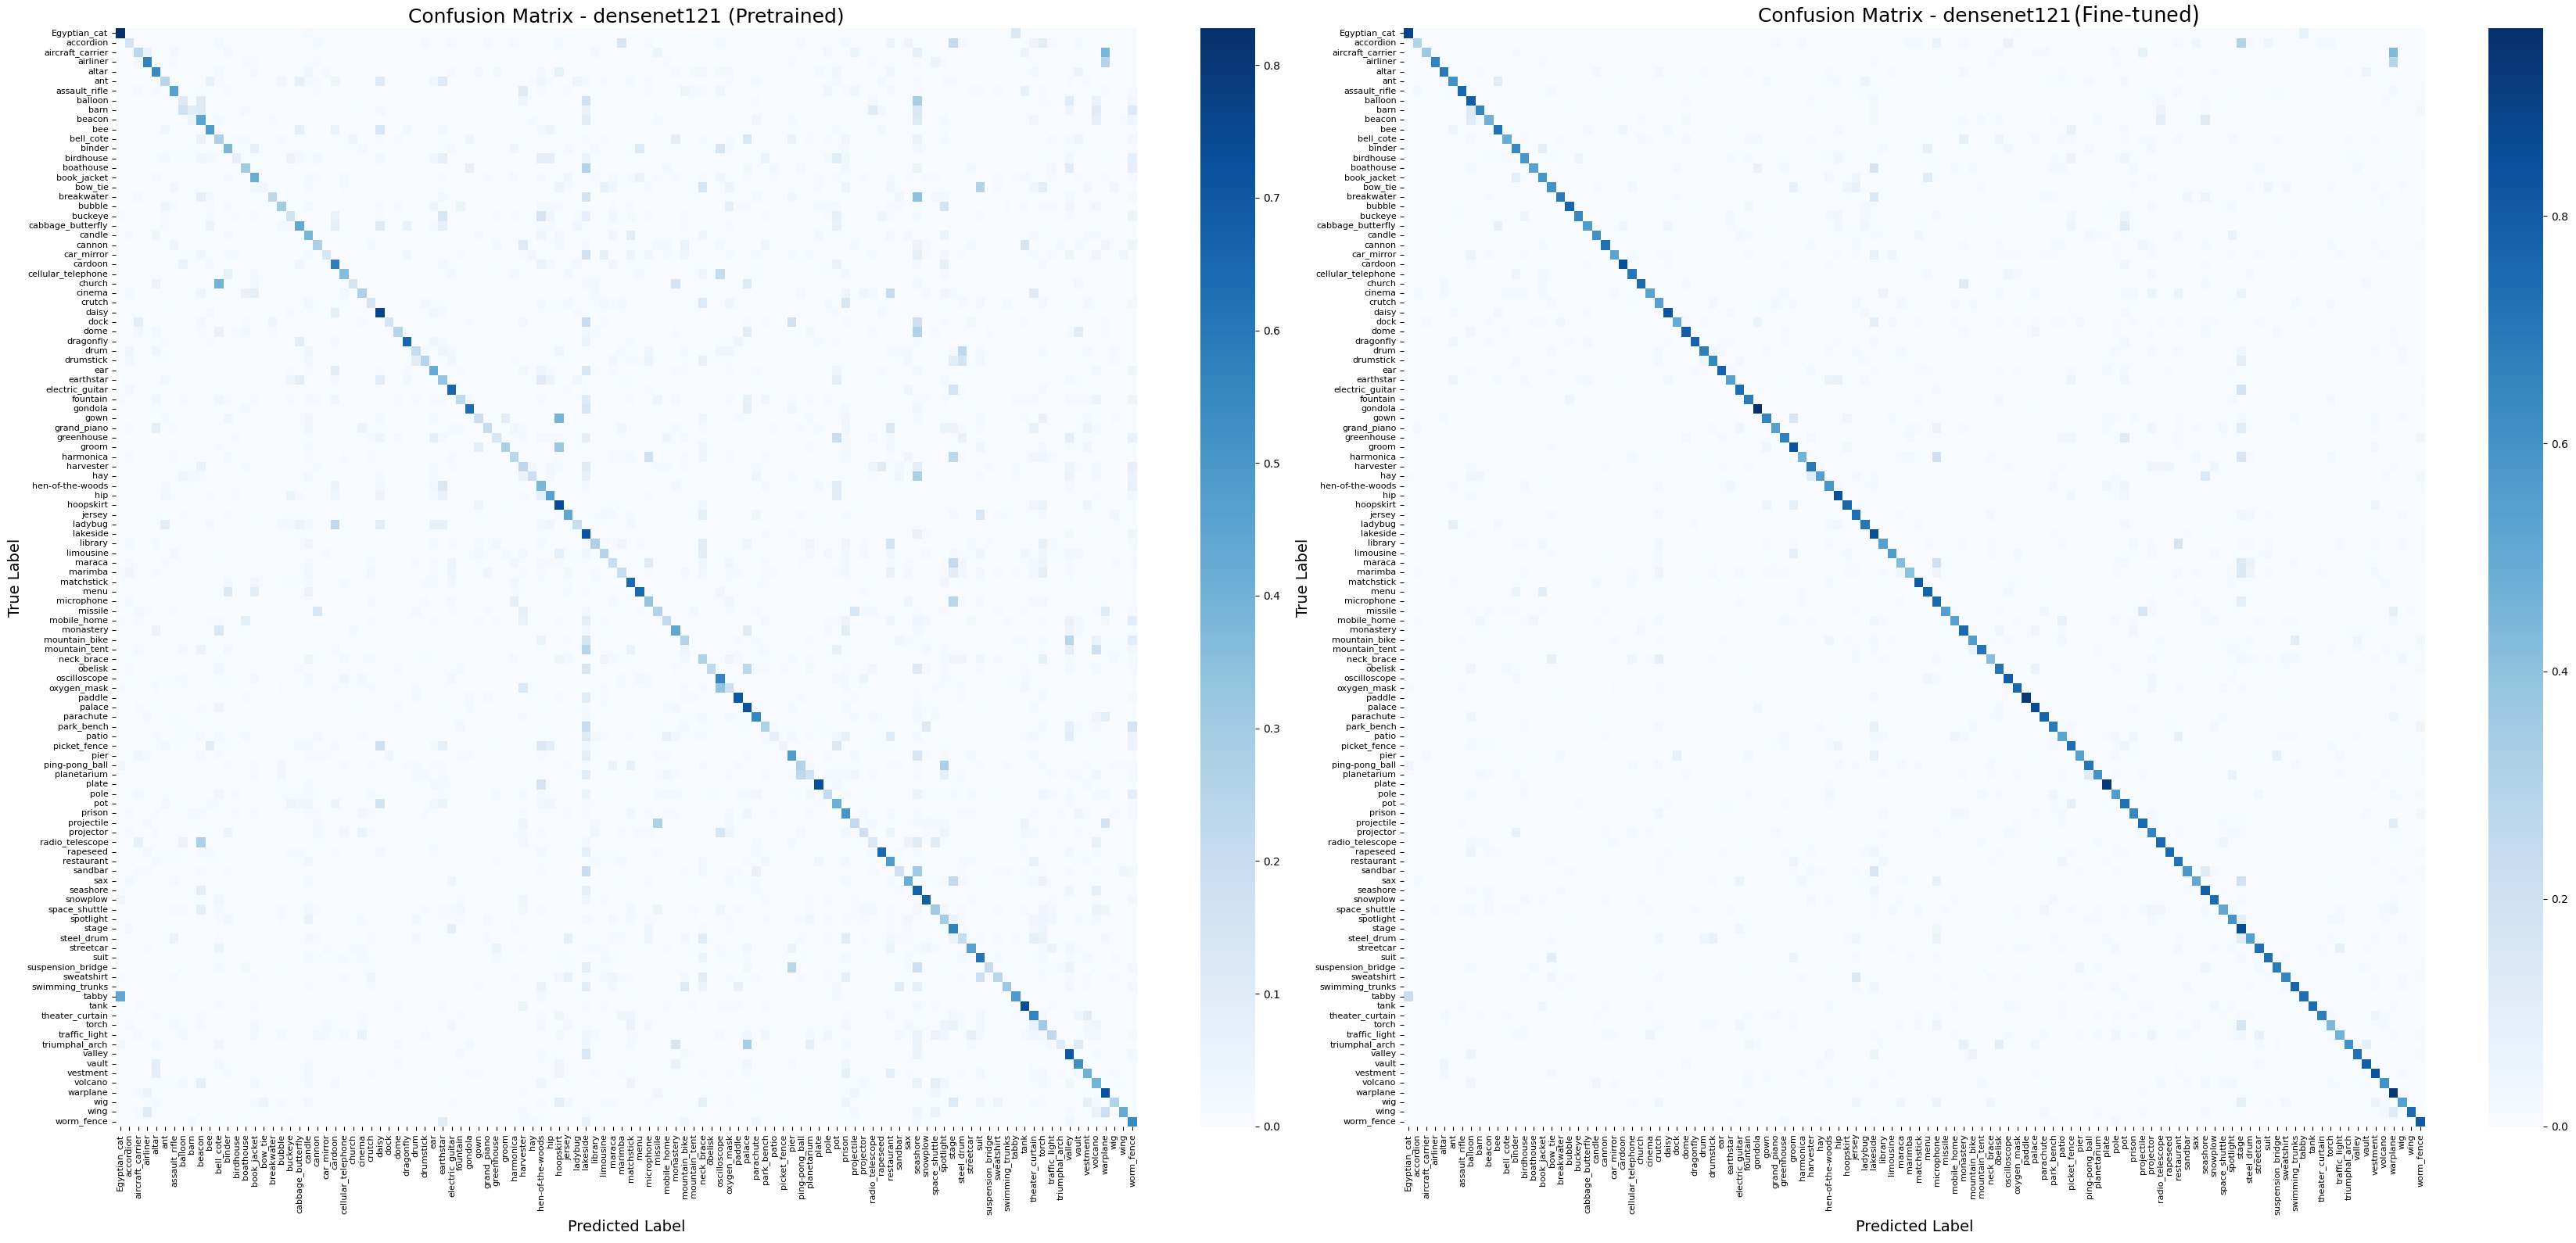
\includegraphics[width=1.0\textwidth]{images/phase02/phase02_DenseNet121_normalised_conf_mat_compare.png}
      \caption{DenseNet121 normalizált Confusion Mátrixok összehasonlítása}
      \label{fig:phase02_DenseNet121_normalised_conf_mat_compare}
    \end{figure}

    \section{EfficientNet-B0}
    \subsubsection{EfficientNet-B0 teljes tanítás folyamata}
    \begin{figure}[H]
      \centering
      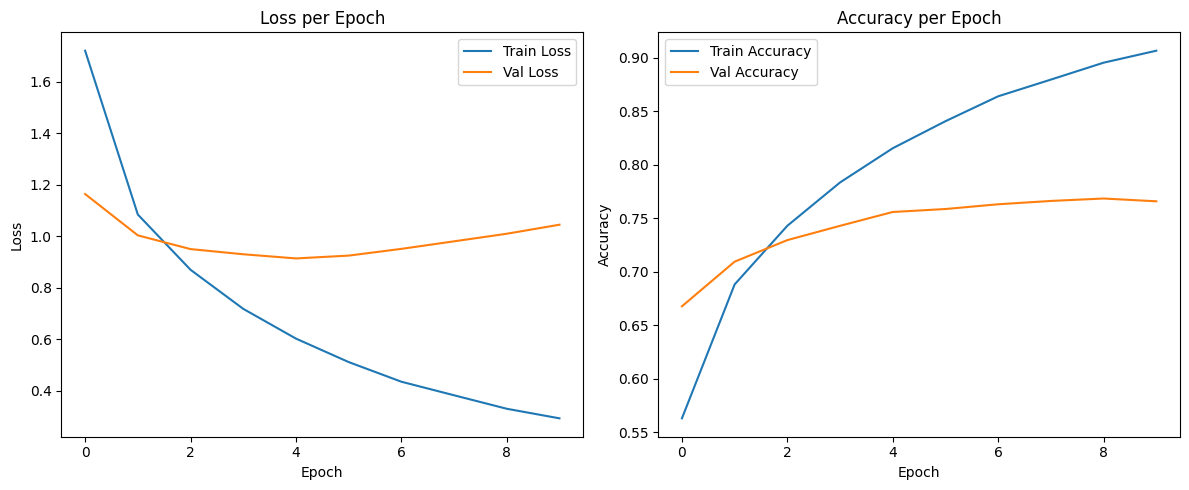
\includegraphics[width=1.0\textwidth]{images/phase02/EfficientNet-B0_learning_curve.png}
      \caption{EfficientNet-B0 teljes tanítás utáni sima Confusion Mátrix}
      \label{fig:phase02_EfficientNet-B0_learning_curves}
    \end{figure}
  
  \subsubsection{EfficientNet-B0 teljes tanítás utáni eredményei}
    \begin{center}
    \begin{longtable}{l c}
    \caption{EfficientNet-B0 teljes tanítás utáni vizsgálati eredményei} \label{tab:phase02_EfficientNet-B0} \\
    \toprule
    \textbf{Metrika} & \textbf{Érték} \\
    \midrule
    \endfirsthead
    \toprule
    \textbf{Metrika} & \textbf{Érték} \\
    \midrule
    \endhead
    Top-1 Accuracy & 0.7649 \\
    Top-5 Accuracy & 0.9421 \\
    Precision & 0.7130 \\
    Recall & 0.6950 \\
    F1-score & 0.7001 \\
    Inference time & 25.26 sec \\
    \bottomrule
    \end{longtable}
    \end{center}
  
  \subsubsection{EfficientNet-B0 eredményeinek összehasonlítása}
    \begin{center}
    \begin{longtable}{l c c}
    \caption{EfficientNet-B0 eredményeinek összehasonlítása} \label{tab:phase02_EfficientNet-B0_compare} \\
    \toprule
    \textbf{Metrika} & \textbf{Pretrained} & \textbf{Fine-tuned} \\
    \midrule
    \endfirsthead
    \toprule
    \textbf{Metrika} & \textbf{Pretrained} & \textbf{Fine-tuned} \\
    \midrule
    \endhead
    Top-1 Accuracy  & 0.4802 & 0.7649 \\
    Top-5 Accuracy & 0.8217 & 0.9421 \\
    Precision & 0.4137 & 0.7130 \\
    Recall & 0.4039 & 0.6950 \\
    F1-score & 0.3829 & 0.7001 \\
    Inference time & 28.89 sec & 25.26 sec \\
    \bottomrule
    \end{longtable}
    \end{center}
  
  \subsubsection{EfficientNet-B0 eredményeinek összehasonlítása}
    \begin{figure}[H]
      \centering
      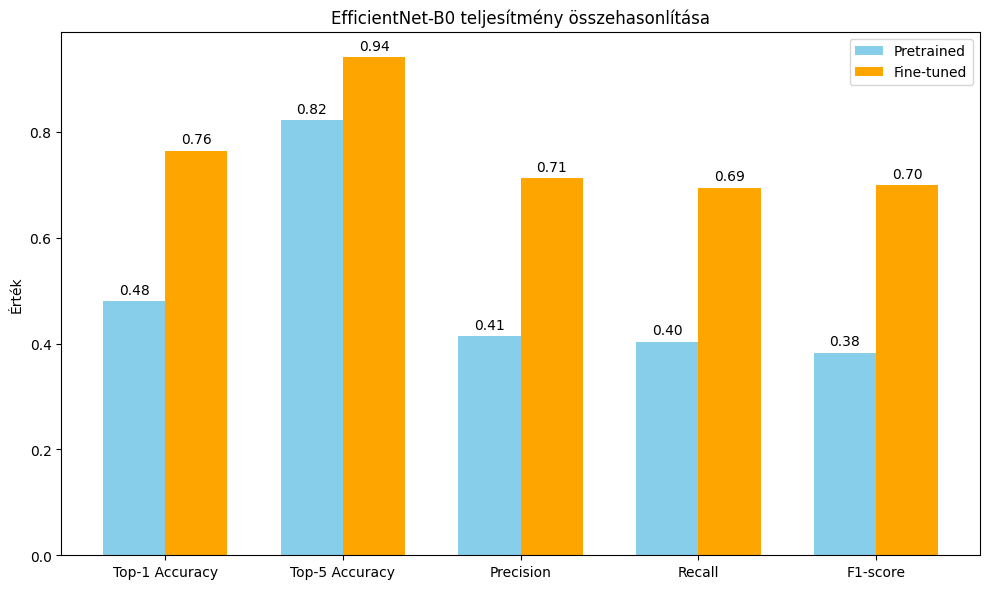
\includegraphics[width=1.0\textwidth]{images/phase02/EfficientNet-B0_compare01.png}
      \caption{EfficientNet-B0 eredményeinek összehasonlítása}
      \label{fig:EfficientNet-B0_compare01}
    \end{figure}
  
  \subsubsection{EfficientNet-B0 eredményeinek összehasonlítása}
    \begin{figure}[H]
      \centering
      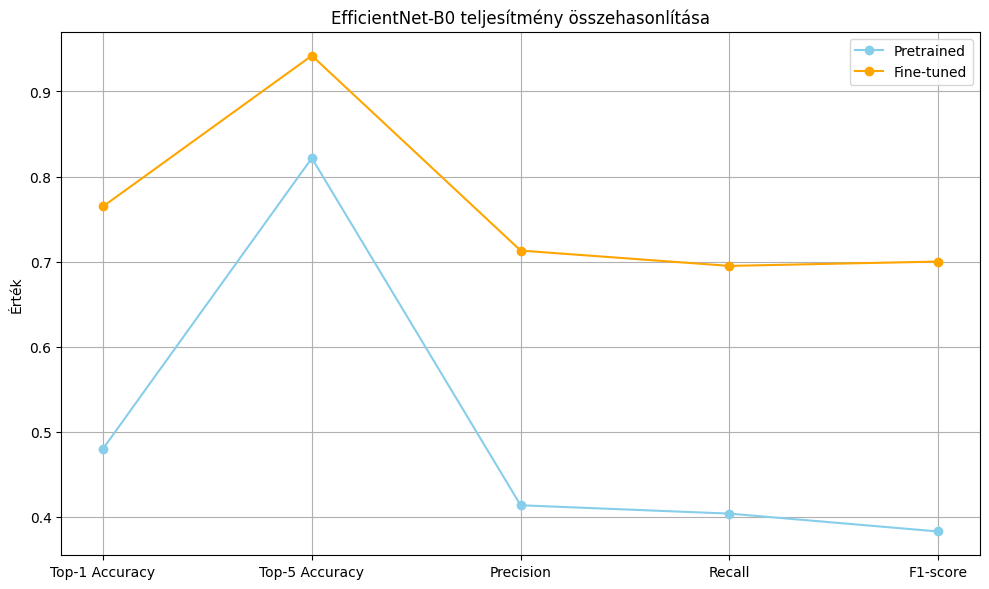
\includegraphics[width=1.0\textwidth]{images/phase02/EfficientNet-B0_compare02.png}
      \caption{EfficientNet-B0 eredményeinek összehasonlítása}
      \label{fig:EfficientNet-B0_compare02}
    \end{figure}

    \subsubsection{EfficientNet-B0 teljes tanítás utáni normalizált Confusion Mátrix}
    \begin{figure}[H]
      \centering
      
\includegraphics[width=0.8\textwidth]{images/phase02/EfficientNet-B0_normalised_conf_mat.png}
      \caption{EfficientNet-B0 teljes tanítás utáni normalizált Confusion Mátrix}
      \label{fig:phase02_EfficientNet-B0_normalised_conf_mat}
    \end{figure}
  
    \subsubsection{EfficientNet-B0 normalizált Confusion Mátrixok összehasonlítása}
    \begin{figure}[H]
      \centering
      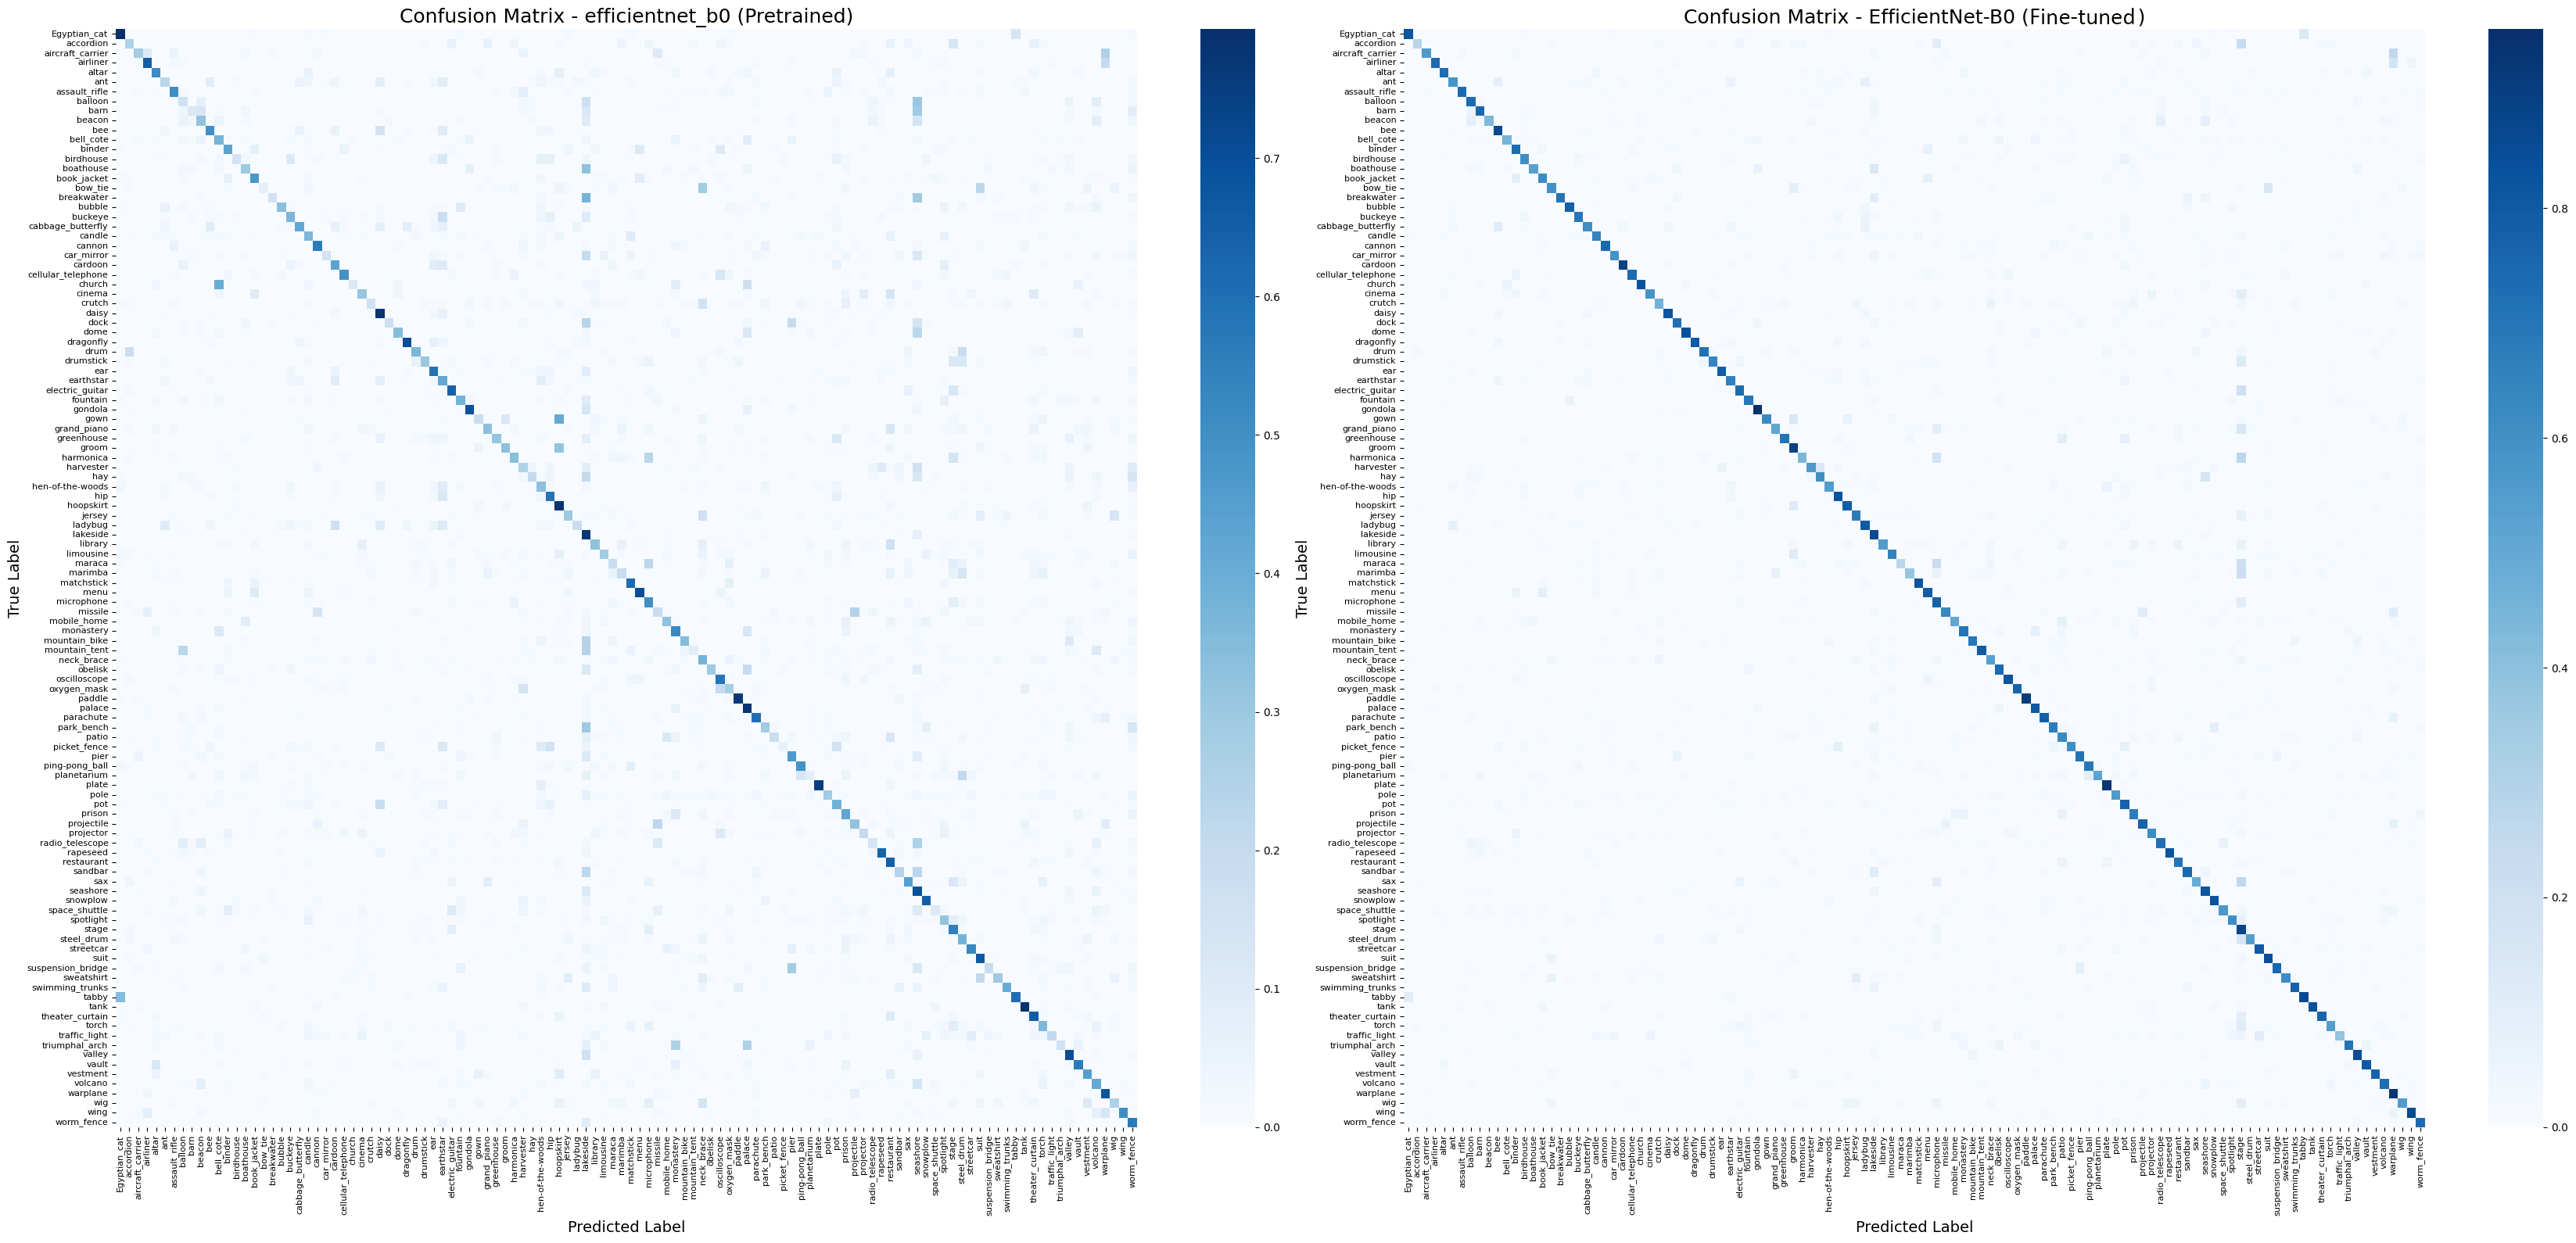
\includegraphics[width=1.0\textwidth]{images/phase02/EfficientNet-B0_normalised_conf_mat_compare.png}
      \caption{EfficientNet-B0 normalizált Confusion Mátrixok összehasonlítása}
      \label{fig:phase02_EfficientNet-B0_normalised_conf_mat_compare}
    \end{figure}

    \section{ConvNeXt-Tiny}
    \subsubsection{ConvNeXt-Tiny teljes tanítás folyamata}
    \begin{figure}[H]
      \centering
      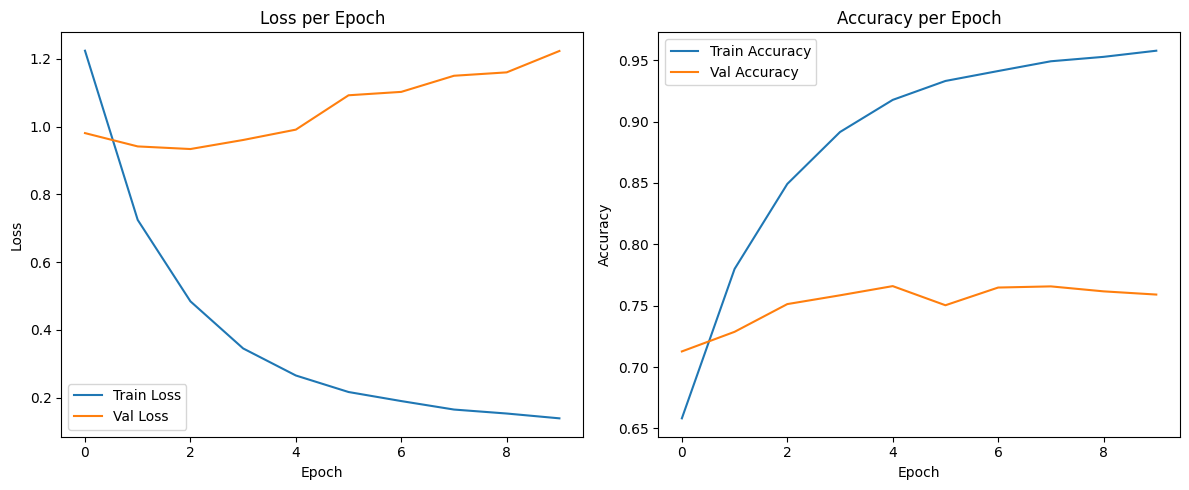
\includegraphics[width=1.0\textwidth]{images/phase02/ConvNeXt-Tiny_learning_curve.png}
      \caption{ConvNeXt-Tiny teljes tanítás utáni sima Confusion Mátrix}
      \label{fig:phase02_ConvNeXt-Tiny_learning_curves}
    \end{figure}
  
  \subsubsection{ConvNeXt-Tiny teljes tanítás utáni eredményei}
    \begin{center}
    \begin{longtable}{l c}
    \caption{ConvNeXt-Tiny teljes tanítás utáni vizsgálati eredményei} \label{tab:phase02_ConvNeXt-Tiny} \\
    \toprule
    \textbf{Metrika} & \textbf{Érték} \\
    \midrule
    \endfirsthead
    \toprule
    \textbf{Metrika} & \textbf{Érték} \\
    \midrule
    \endhead
    Top-1 Accuracy & 0.7624 \\
    Top-5 Accuracy & 0.9357 \\
    Precision & 0.7168 \\
    Recall & 0.6841 \\
    F1-score & 0.6947 \\
    Inference time & 25.67 sec \\
    \bottomrule
    \end{longtable}
    \end{center}
  
  \subsubsection{ConvNeXt-Tiny eredményeinek összehasonlítása}
    \begin{center}
    \begin{longtable}{l c c}
    \caption{ConvNeXt-Tiny eredményeinek összehasonlítása} \label{tab:phase02_ConvNeXt-Tiny_compare} \\
    \toprule
    \textbf{Metrika} & \textbf{Pretrained} & \textbf{Fine-tuned} \\
    \midrule
    \endfirsthead
    \toprule
    \textbf{Metrika} & \textbf{Pretrained} & \textbf{Fine-tuned} \\
    \midrule
    \endhead
    Top-1 Accuracy  & 0.5048 & 0.7624 \\
    Top-5 Accuracy & 0.8471 & 0.9357 \\
    Precision & 0.4917 & 0.7168 \\
    Recall & 0.4369 & 0.6841 \\
    F1-score & 0.4194 & 0.6947 \\
    Inference time & 38.40 sec & 25.67 sec \\
    \bottomrule
    \end{longtable}
    \end{center}
  
  \subsubsection{ConvNeXt-Tiny eredményeinek összehasonlítása}
    \begin{figure}[H]
      \centering
      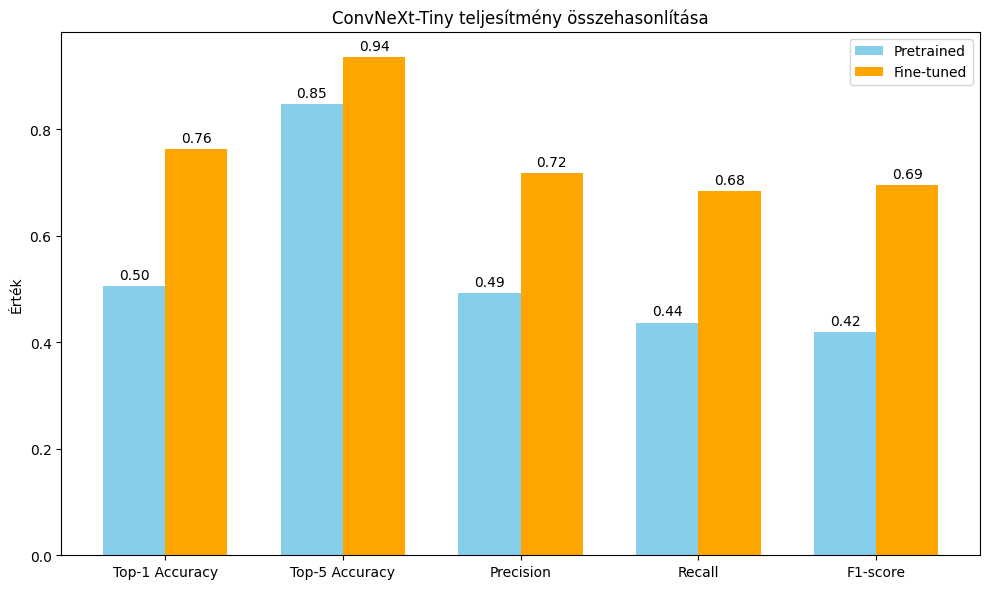
\includegraphics[width=1.0\textwidth]{images/phase02/ConvNeXt-Tiny_compare01.png}
      \caption{ConvNeXt-Tiny eredményeinek összehasonlítása}
      \label{fig:ConvNeXt-Tiny_compare01}
    \end{figure}
  
  \subsubsection{ConvNeXt-Tiny eredményeinek összehasonlítása}
    \begin{figure}[H]
      \centering
      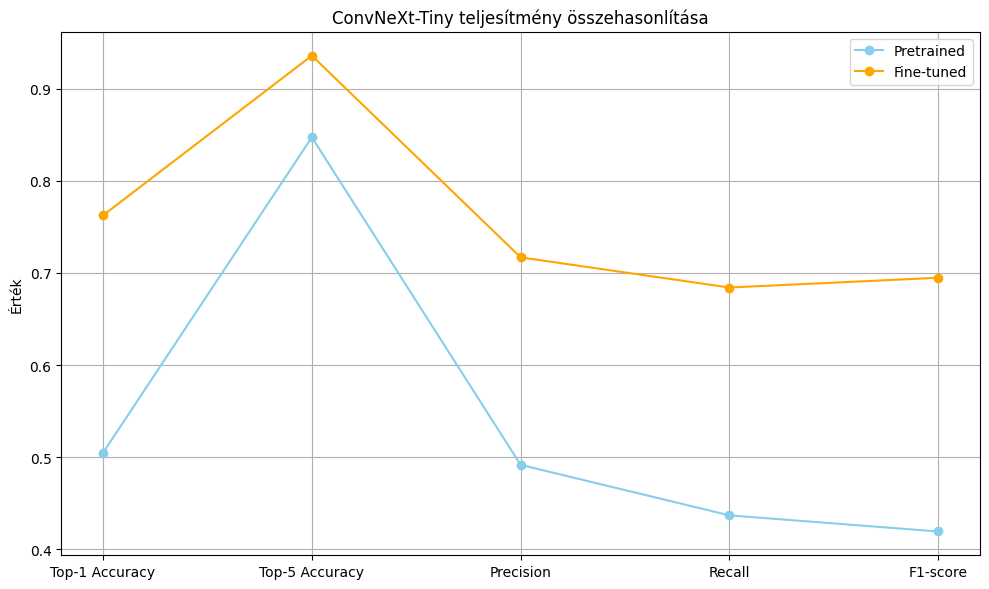
\includegraphics[width=1.0\textwidth]{images/phase02/ConvNeXt-Tiny_compare02.png}
      \caption{ConvNeXt-Tiny eredményeinek összehasonlítása}
      \label{fig:ConvNeXt-Tiny_compare02}
    \end{figure}

    \subsubsection{ConvNeXt-Tiny teljes tanítás utáni normalizált Confusion Mátrix}
    \begin{figure}[H]
      \centering
      
\includegraphics[width=0.8\textwidth]{images/phase02/ConvNeXt-Tiny_normalised_conf_mat.png}
      \caption{ConvNeXt-Tiny teljes tanítás utáni normalizált Confusion Mátrix}
      \label{fig:phase02_ConvNeXt-Tiny_normalised_conf_mat}
    \end{figure}
  
    \subsubsection{ConvNeXt-Tiny normalizált Confusion Mátrixok összehasonlítása}
    \begin{figure}[H]
      \centering
      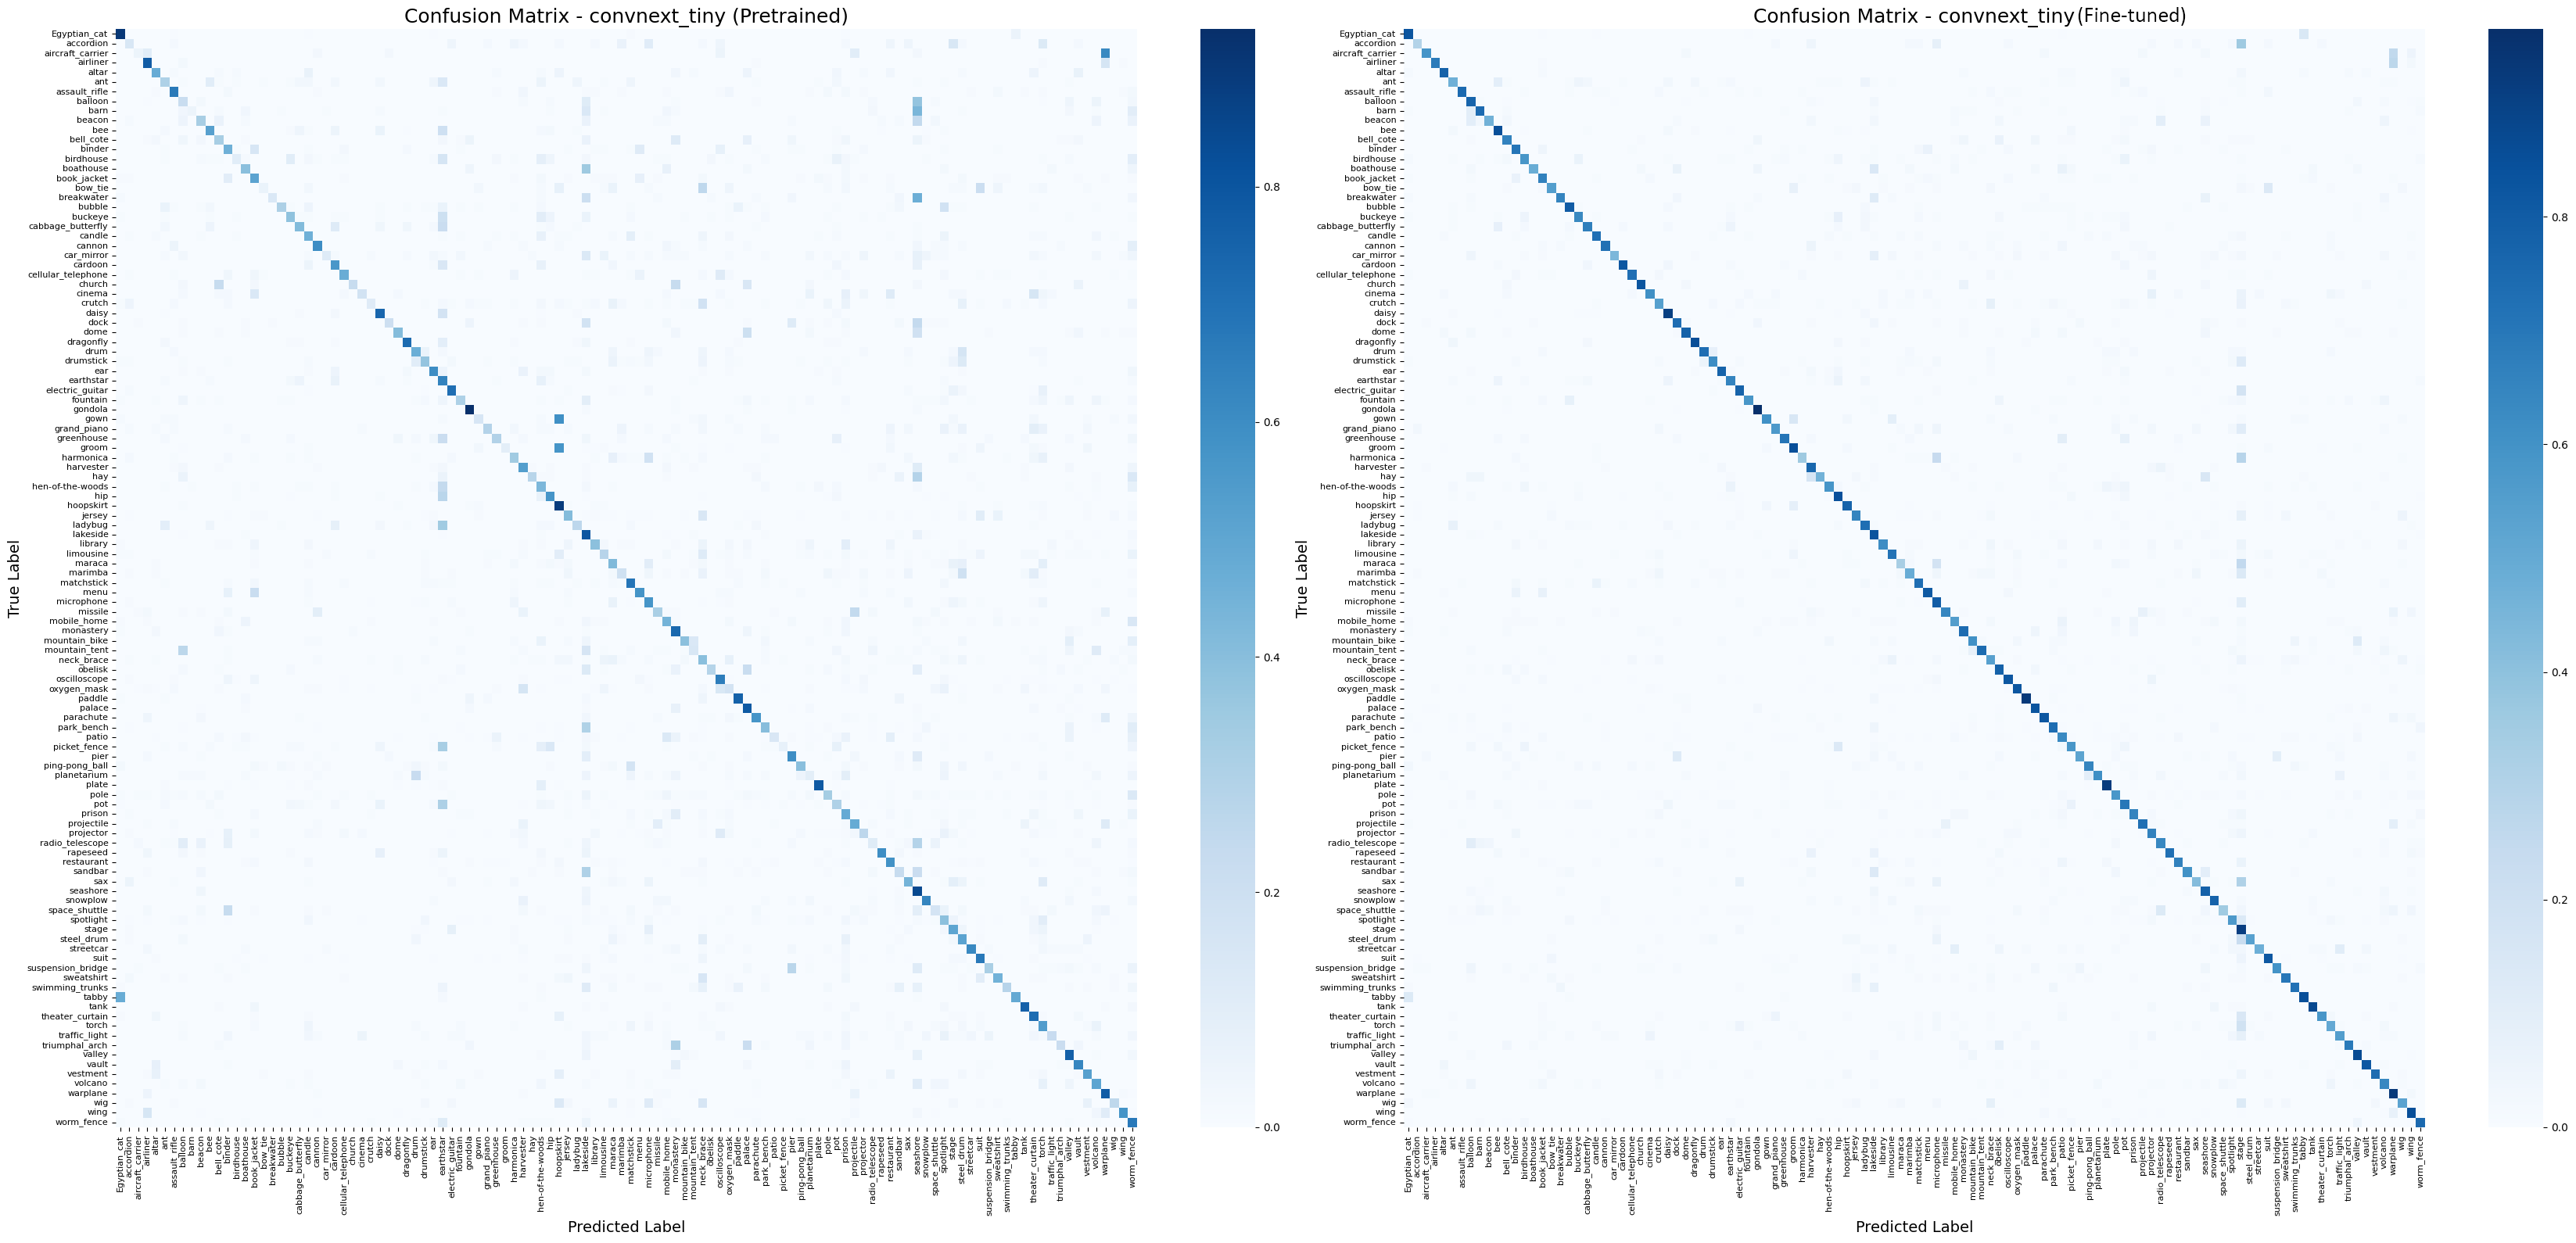
\includegraphics[width=1.0\textwidth]{images/phase02/ConvNeXt-Tiny_normalised_conf_mat_compare.png}
      \caption{ConvNeXt-Tiny normalizált Confusion Mátrixok összehasonlítása}
      \label{fig:phase02_ConvNeXt-Tiny_normalised_conf_mat_compare}
    \end{figure}


    \section{ViT-B/16}
    \subsubsection{ViT-B-16 teljes tanítás folyamata}
  \begin{figure}[H]
    \centering
    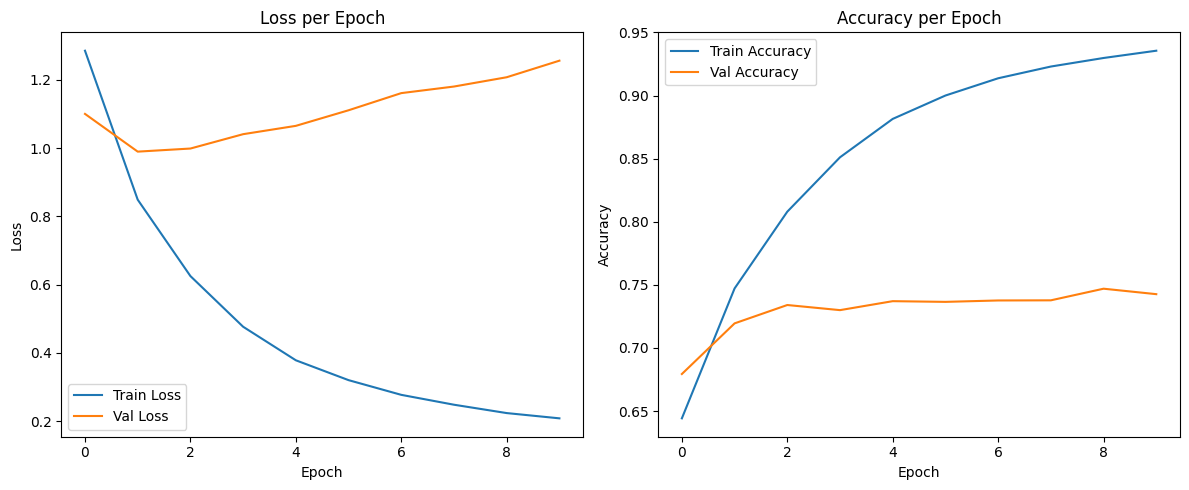
\includegraphics[width=1.0\textwidth]{images/phase02/ViT-B-16_learning_curve.png}
    \caption{ViT-B-16 teljes tanítás utáni sima Confusion Mátrix}
    \label{fig:phase02_ViT-B-16_learning_curves}
  \end{figure}

\subsubsection{ViT-B-16 teljes tanítás utáni eredményei}
  \begin{center}
  \begin{longtable}{l c}
  \caption{ViT-B-16 teljes tanítás utáni vizsgálati eredményei} \label{tab:phase02_ViT-B-16} \\
  \toprule
  \textbf{Metrika} & \textbf{Érték} \\
  \midrule
  \endfirsthead
  \toprule
  \textbf{Metrika} & \textbf{Érték} \\
  \midrule
  \endhead
  Top-1 Accuracy & 0.7414 \\
  Top-5 Accuracy & 0.9257 \\
  Precision & 0.6935 \\
  Recall & 0.6636 \\
  F1-score & 0.6730 \\
  Inference time & 42.40 sec \\
  \bottomrule
  \end{longtable}
  \end{center}

\subsubsection{ViT-B-16 eredményeinek összehasonlítása}
  \begin{center}
  \begin{longtable}{l c c}
  \caption{ViT-B-16 eredményeinek összehasonlítása} \label{tab:phase02_ViT-B-16_compare} \\
  \toprule
  \textbf{Metrika} & \textbf{Pretrained} & \textbf{Fine-tuned} \\
  \midrule
  \endfirsthead
  \toprule
  \textbf{Metrika} & \textbf{Pretrained} & \textbf{Fine-tuned} \\
  \midrule
  \endhead
  Top-1 Accuracy  & 0.5308 & 0.7414 \\
  Top-5 Accuracy & 0.8582 & 0.9257 \\
  Precision & 0.4629 & 0.6935 \\
  Recall & 0.4419 & 0.6636 \\
  F1-score & 0.4307 & 0.6908 \\
  Inference time & 92.13 sec & 42.40 sec \\
  \bottomrule
  \end{longtable}
  \end{center}

\subsubsection{ViT-B-16 eredményeinek összehasonlítása}
  \begin{figure}[H]
    \centering
    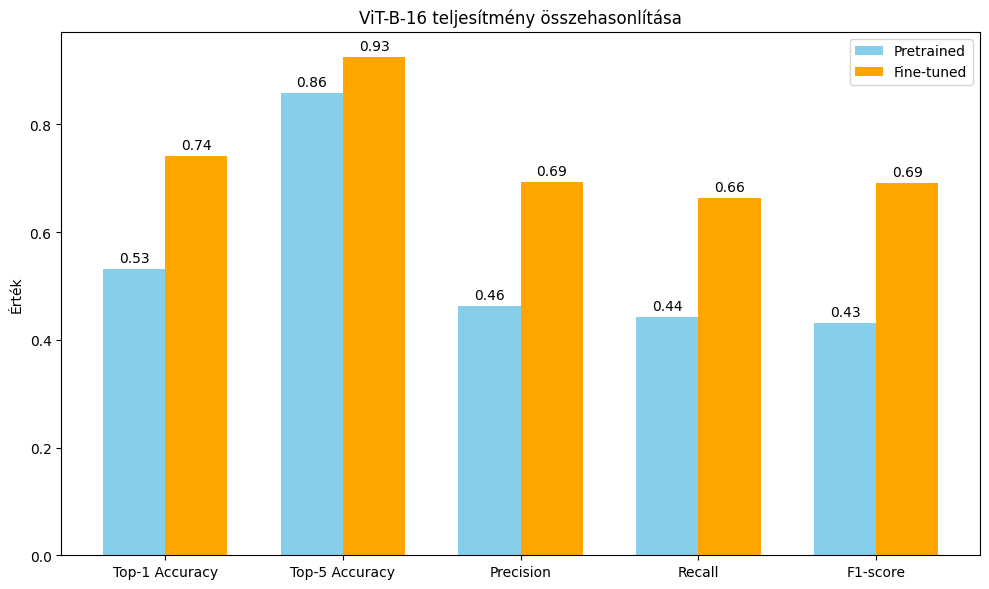
\includegraphics[width=1.0\textwidth]{images/phase02/ViT-B-16_compare01.png}
    \caption{ViT-B-16 eredményeinek összehasonlítása}
    \label{fig:ViT-B-16_compare01}
  \end{figure}

\subsubsection{ViT-B-16 eredményeinek összehasonlítása}
  \begin{figure}[H]
    \centering
    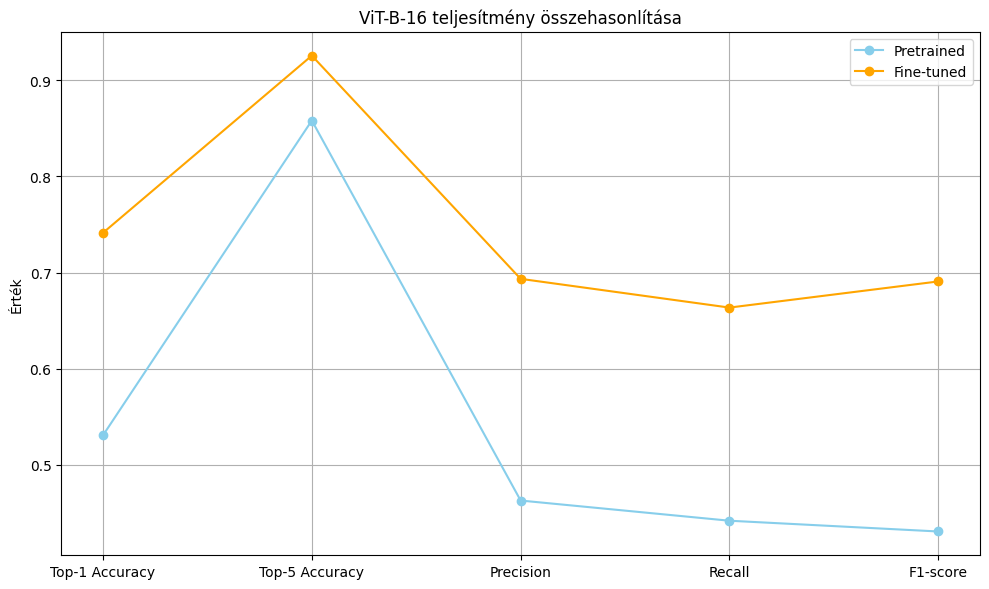
\includegraphics[width=1.0\textwidth]{images/phase02/ViT-B-16_compare02.png}
    \caption{ViT-B-16 eredményeinek összehasonlítása}
    \label{fig:ViT-B-16_compare02}
  \end{figure}

  \subsubsection{ViT-B-16 teljes tanítás utáni normalizált Confusion Mátrix}
  \begin{figure}[H]
    \centering
    
\includegraphics[width=0.8\textwidth]{images/phase02/ViT-B-16_normalised_conf_mat.png}
    \caption{ViT-B-16 teljes tanítás utáni normalizált Confusion Mátrix}
    \label{fig:phase02_ViT-B-16_normalised_conf_mat}
  \end{figure}

  \subsubsection{ViT-B-16 normalizált Confusion Mátrixok összehasonlítása}
  \begin{figure}[H]
    \centering
    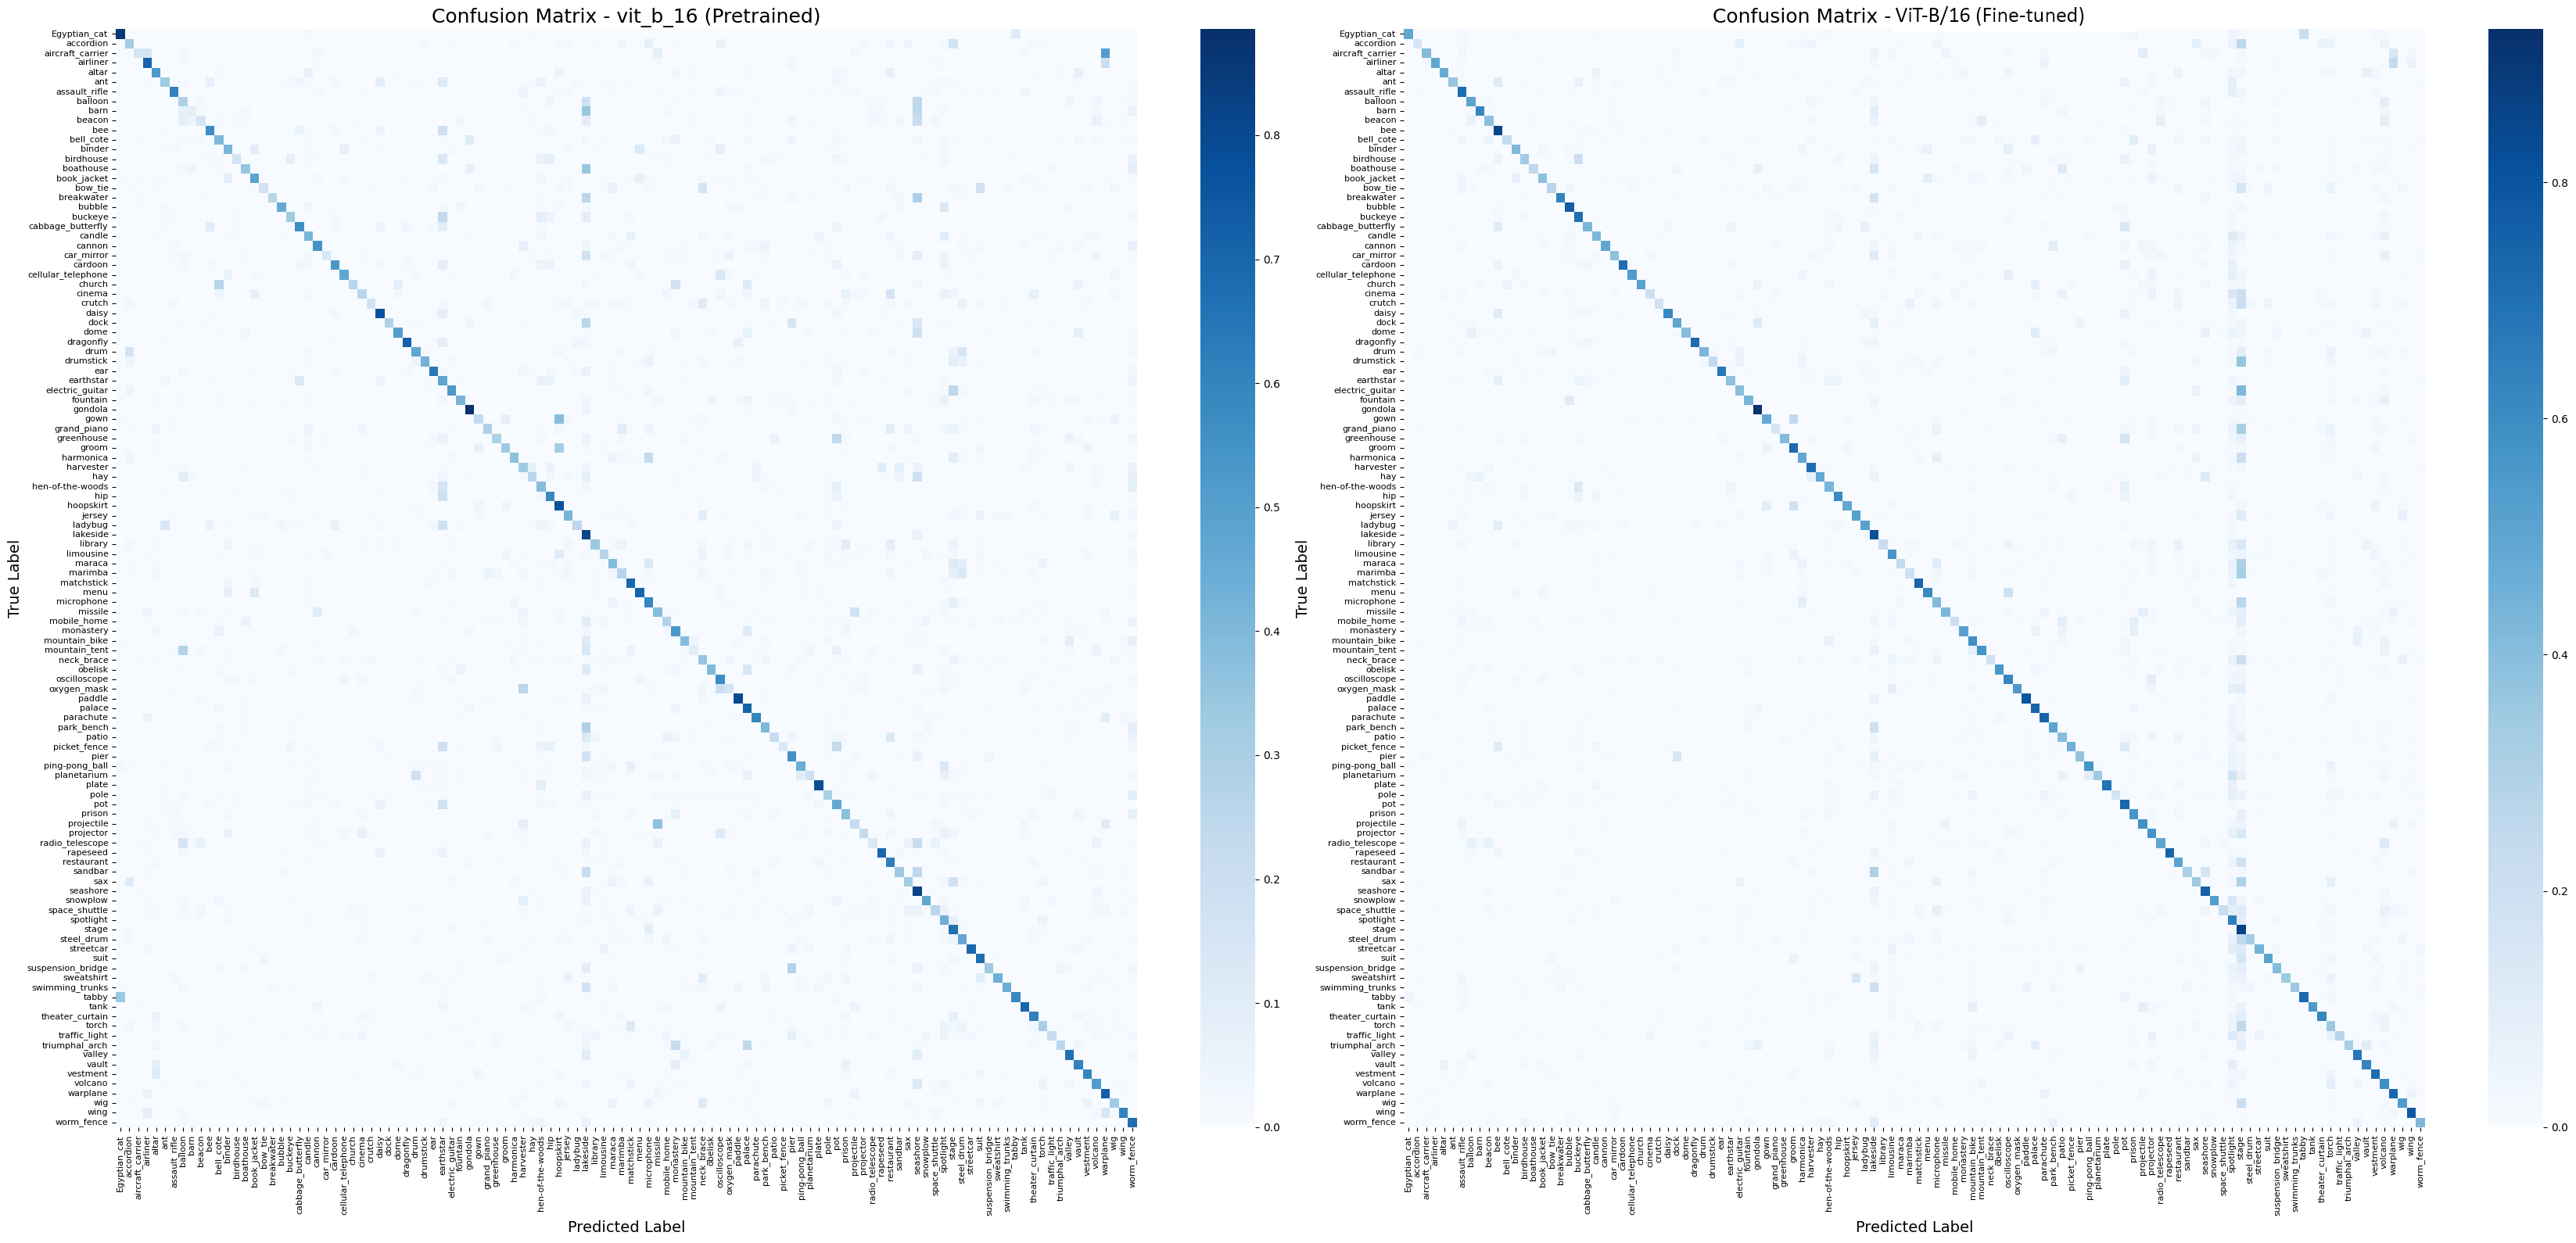
\includegraphics[width=1.0\textwidth]{images/phase02/ViT-B-16_normalised_conf_mat_compare.png}
    \caption{ViT-B-16 normalizált Confusion Mátrixok összehasonlítása}
    \label{fig:phase02_ViT-B-16_normalised_conf_mat_compare}
  \end{figure}


    \section{Inception-v3}
    \subsubsection{Inception-v3 teljes tanítás folyamata}
  \begin{figure}[H]
    \centering
    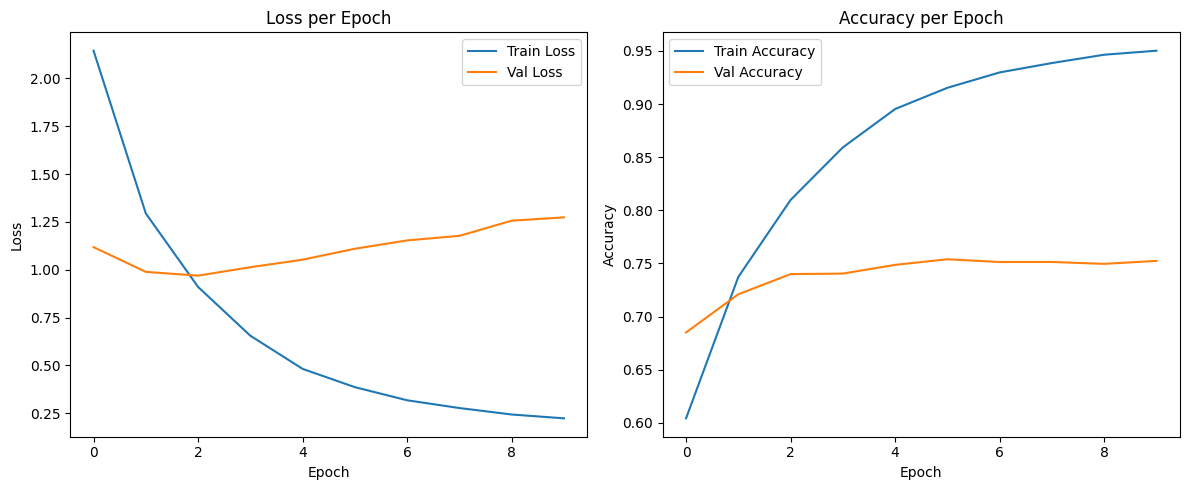
\includegraphics[width=1.0\textwidth]{images/phase02/Inception-v3_learning_curve.png}
    \caption{Inception-v3 teljes tanítás utáni sima Confusion Mátrix}
    \label{fig:phase02_Inception-v3_learning_curves}
  \end{figure}

\subsubsection{Inception-v3 teljes tanítás utáni eredményei}
  \begin{center}
  \begin{longtable}{l c}
  \caption{Inception-v3 teljes tanítás utáni vizsgálati eredményei} \label{tab:phase02_Inception-v3} \\
  \toprule
  \textbf{Metrika} & \textbf{Érték} \\
  \midrule
  \endfirsthead
  \toprule
  \textbf{Metrika} & \textbf{Érték} \\
  \midrule
  \endhead
  Top-1 Accuracy & 0.7518 \\
  Top-5 Accuracy & 0.9320 \\
  Precision & 0.6963 \\
  Recall & 0.6787 \\
  F1-score & 0.6908 \\
  Inference time & 25.11 sec \\
  \bottomrule
  \end{longtable}
  \end{center}

\subsubsection{Inception-v3 eredményeinek összehasonlítása}
  \begin{center}
  \begin{longtable}{l c c}
  \caption{Inception-v3 eredményeinek összehasonlítása} \label{tab:phase02_Inception-v3_compare} \\
  \toprule
  \textbf{Metrika} & \textbf{Pretrained} & \textbf{Fine-tuned} \\
  \midrule
  \endfirsthead
  \toprule
  \textbf{Metrika} & \textbf{Pretrained} & \textbf{Fine-tuned} \\
  \midrule
  \endhead
  Top-1 Accuracy  & 0.4763 & 0.7518 \\
  Top-5 Accuracy & 0.8008 & 0.9320 \\
  Precision & 0.3833 & 0.6963 \\
  Recall & 0.3896 & 0.6787 \\
  F1-score & 0.3683 & 0.6827 \\
  Inference time & 38.06 sec & 33.62 sec \\
  \bottomrule
  \end{longtable}
  \end{center}

\subsubsection{Inception-v3 eredményeinek összehasonlítása}
  \begin{figure}[H]
    \centering
    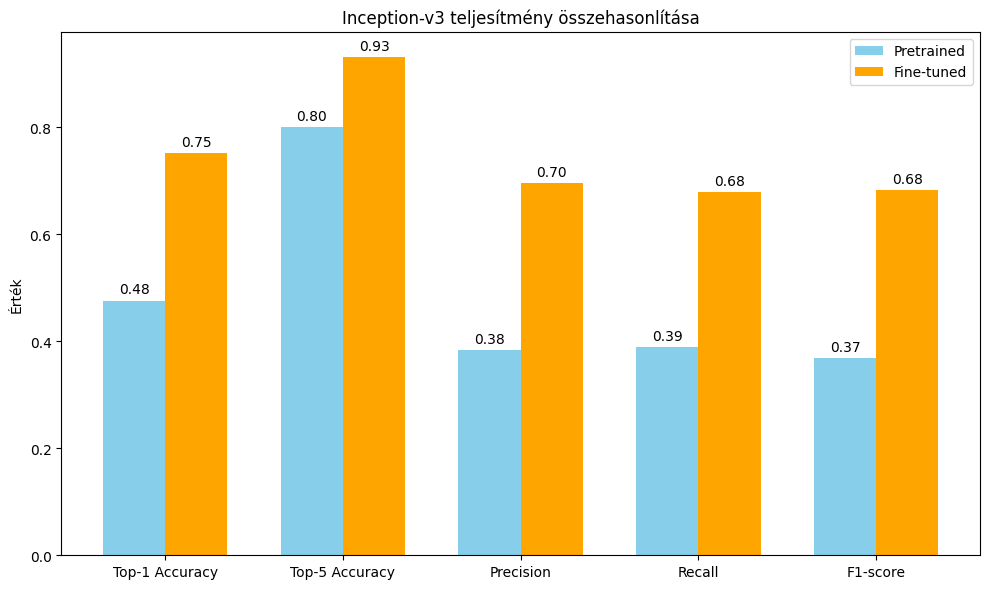
\includegraphics[width=1.0\textwidth]{images/phase02/Inception-v3_compare01.png}
    \caption{Inception-v3 eredményeinek összehasonlítása}
    \label{fig:Inception-v3_compare01}
  \end{figure}

\subsubsection{Inception-v3 eredményeinek összehasonlítása}
  \begin{figure}[H]
    \centering
    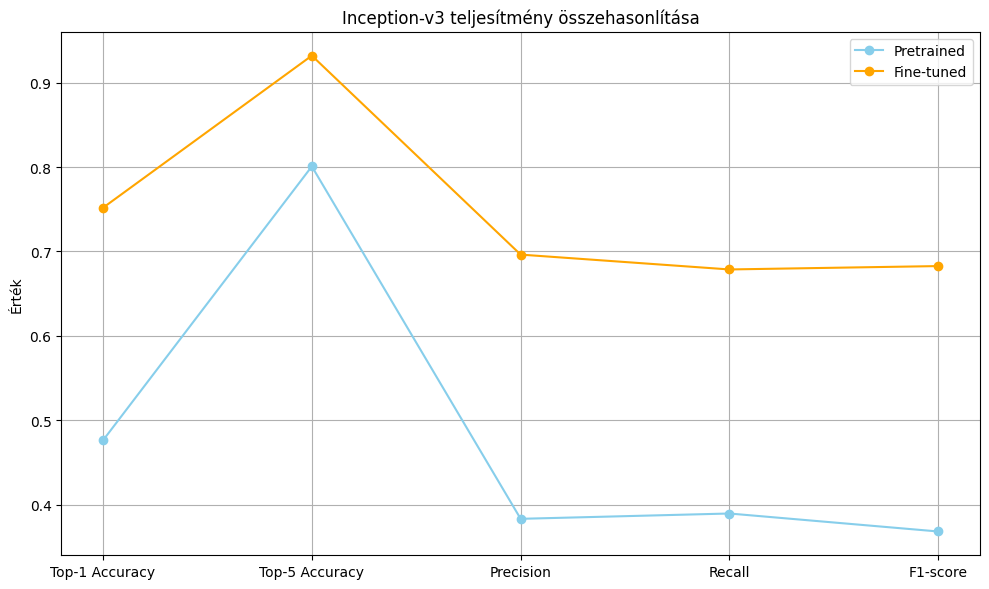
\includegraphics[width=1.0\textwidth]{images/phase02/Inception-v3_compare02.png}
    \caption{Inception-v3 eredményeinek összehasonlítása}
    \label{fig:Inception-v3_compare02}
  \end{figure}

  \subsubsection{Inception-v3 teljes tanítás utáni normalizált Confusion Mátrix}
  \begin{figure}[H]
    \centering
    
\includegraphics[width=0.8\textwidth]{images/phase02/Inception-v3_normalised_conf_mat.png}
    \caption{Inception-v3 teljes tanítás utáni normalizált Confusion Mátrix}
    \label{fig:phase02_Inception-v3_normalised_conf_mat}
  \end{figure}

  \subsubsection{Inception-v3 normalizált Confusion Mátrixok összehasonlítása}
  \begin{figure}[H]
    \centering
    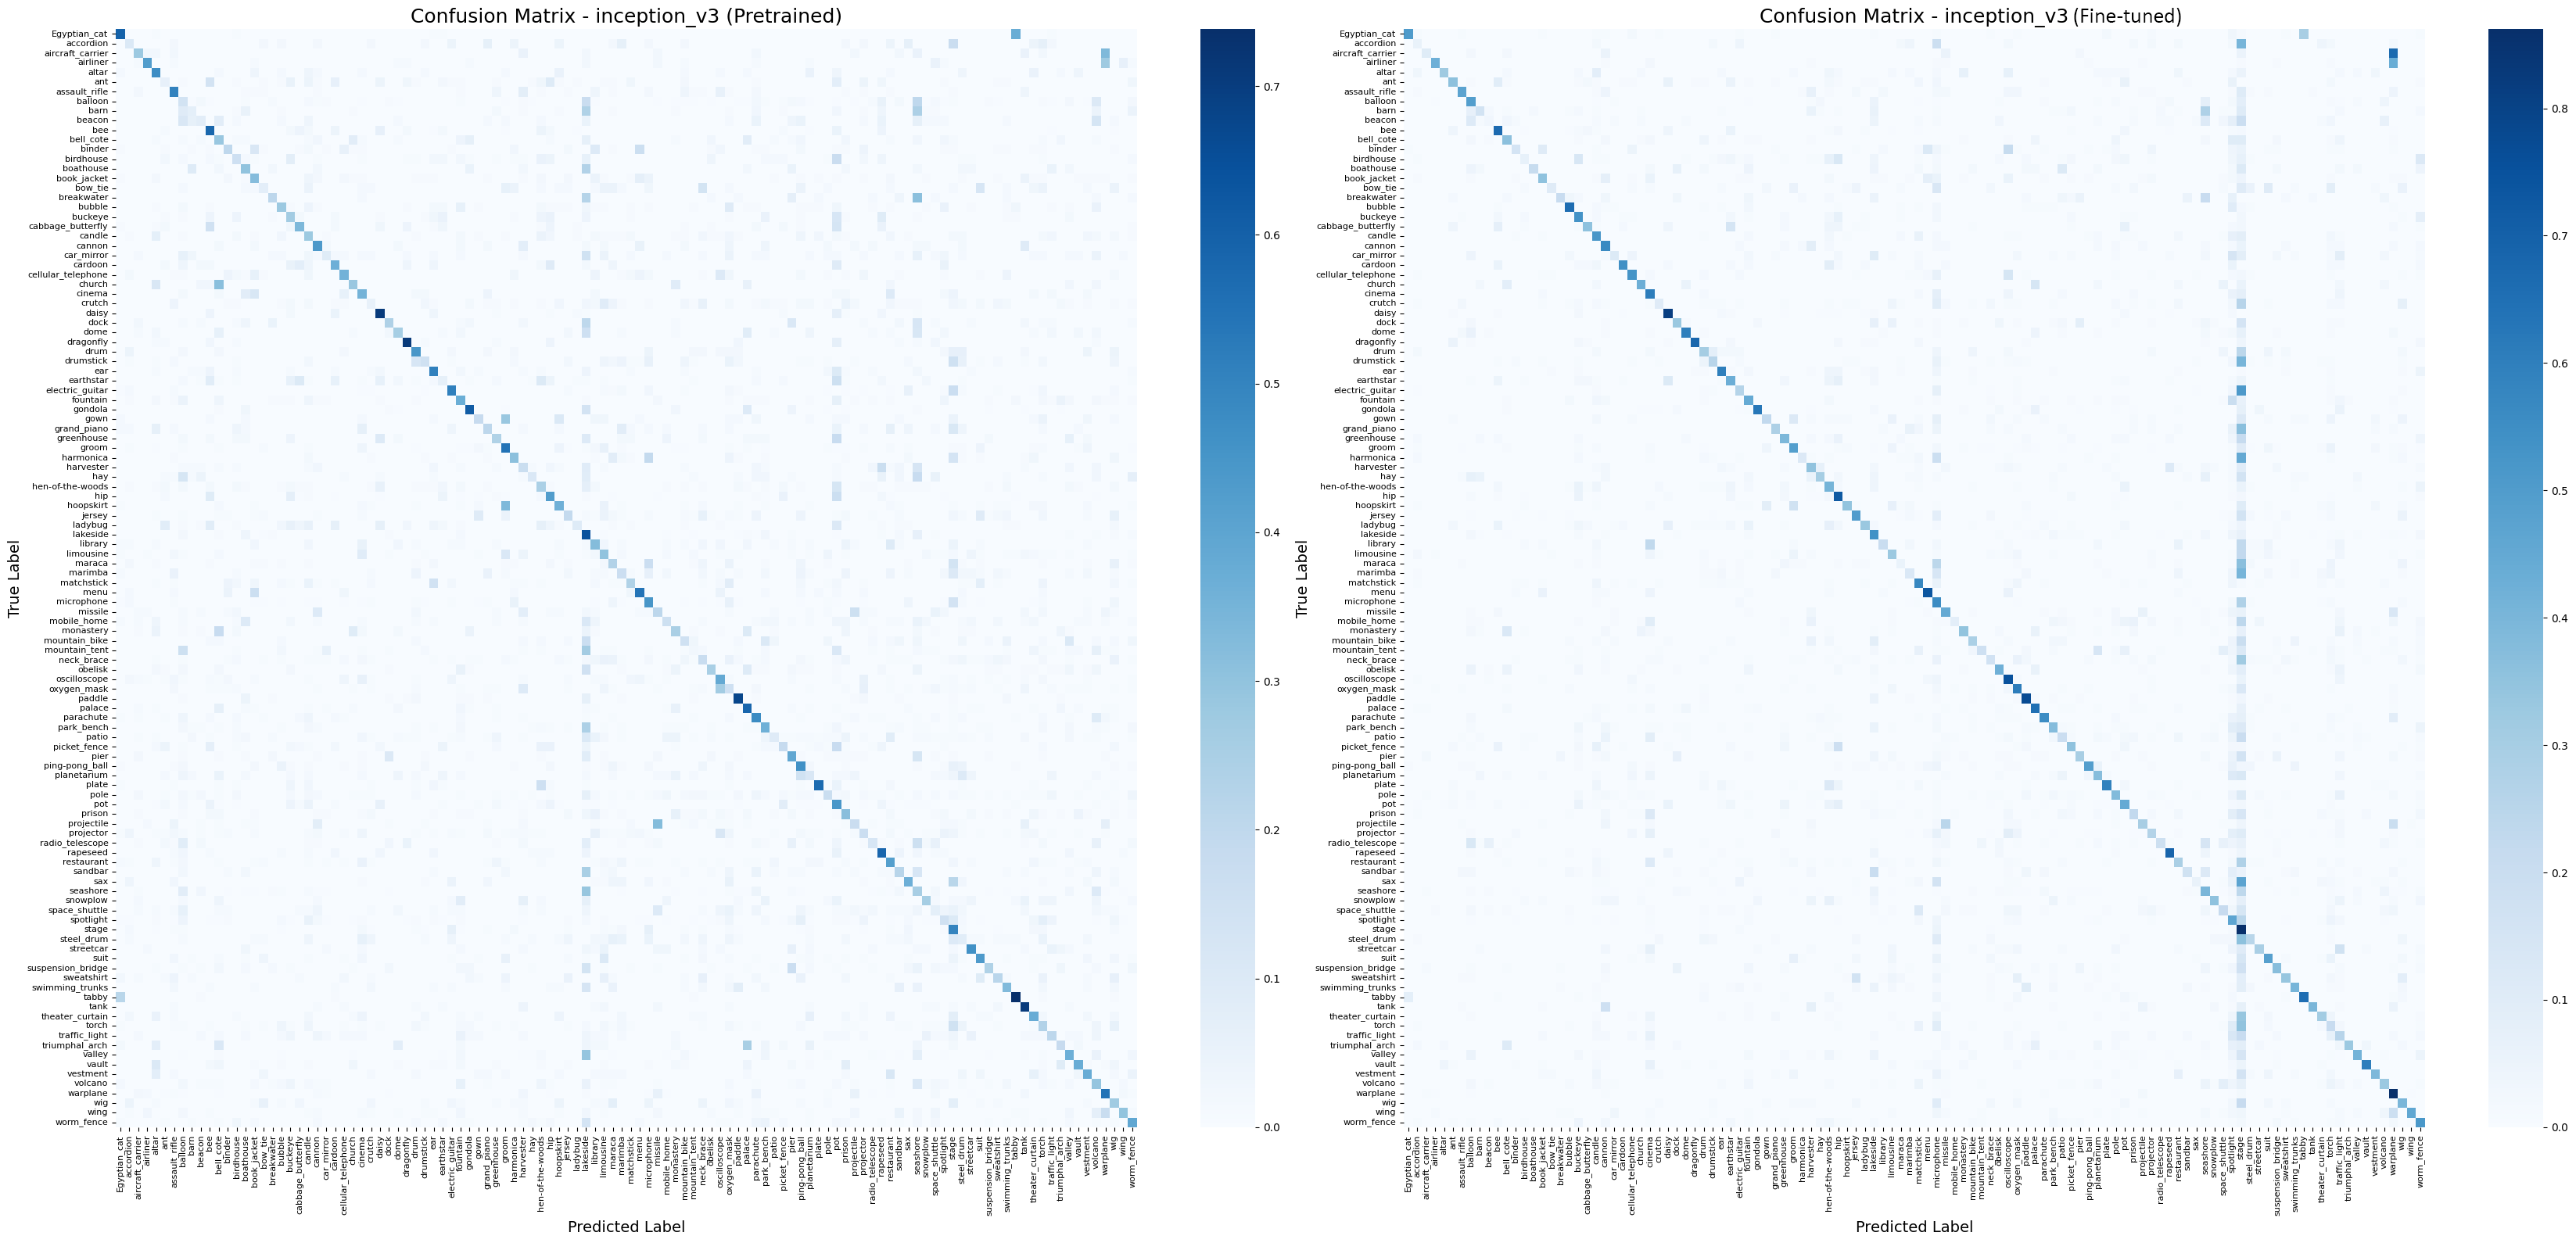
\includegraphics[width=1.0\textwidth]{images/phase02/Inception-v3_normalised_conf_mat_compare.png}
    \caption{Inception-v3 normalizált Confusion Mátrixok összehasonlítása}
    \label{fig:phase02_Inception-v3_normalised_conf_mat_compare}
  \end{figure}


    \section{NASNet}
    \subsubsection{NASNet teljes tanítás folyamata}
  \begin{figure}[H]
    \centering
    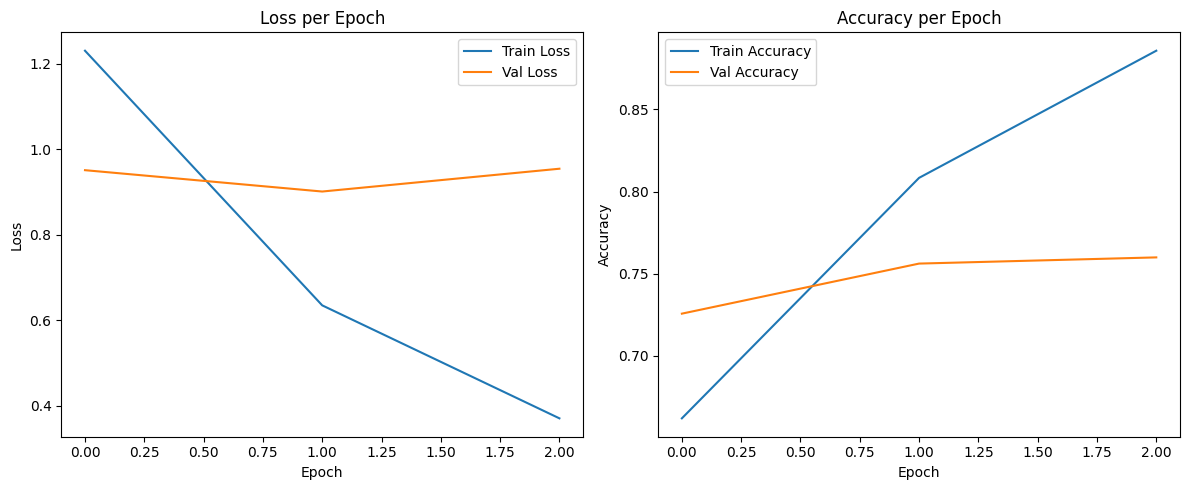
\includegraphics[width=1.0\textwidth]{images/phase02/NASNet_learning_curve.png}
    \caption{NASNet teljes tanítás utáni sima Confusion Mátrix}
    \label{fig:phase02_NASNet_learning_curves}
  \end{figure}

\subsubsection{NASNet teljes tanítás utáni eredményei}
  \begin{center}
  \begin{longtable}{l c}
  \caption{NASNet teljes tanítás utáni vizsgálati eredményei} \label{tab:phase02_NASNet} \\
  \toprule
  \textbf{Metrika} & \textbf{Érték} \\
  \midrule
  \endfirsthead
  \toprule
  \textbf{Metrika} & \textbf{Érték} \\
  \midrule
  \endhead
  Top-1 Accuracy & 0.7626 \\
  Top-5 Accuracy & 0.9470 \\
  Precision & 0.7180 \\
  Recall & 0.6875 \\
  F1-score & 0.6955 \\
  Inference time & 25.11 sec \\
  \bottomrule
  \end{longtable}
  \end{center}

\subsubsection{NASNet eredményeinek összehasonlítása}
  \begin{center}
  \begin{longtable}{l c c}
  \caption{NASNet eredményeinek összehasonlítása} \label{tab:phase02_NASNet_compare} \\
  \toprule
  \textbf{Metrika} & \textbf{Pretrained} & \textbf{Fine-tuned} \\
  \midrule
  \endfirsthead
  \toprule
  \textbf{Metrika} & \textbf{Pretrained} & \textbf{Fine-tuned} \\
  \midrule
  \endhead
  Top-1 Accuracy  & 0.2820 & 0.7626 \\
  Top-5 Accuracy & 0.5408 & 0.9470 \\
  Precision & 0.3204 & 0.7180 \\
  Recall & 0.2799 & 0.6808 \\
  F1-score & 0.2696 & 0.6955 \\
  Inference time & 275.30 sec & 34.03 sec \\
  \bottomrule
  \end{longtable}
  \end{center}

\subsubsection{NASNet eredményeinek összehasonlítása}
  \begin{figure}[H]
    \centering
    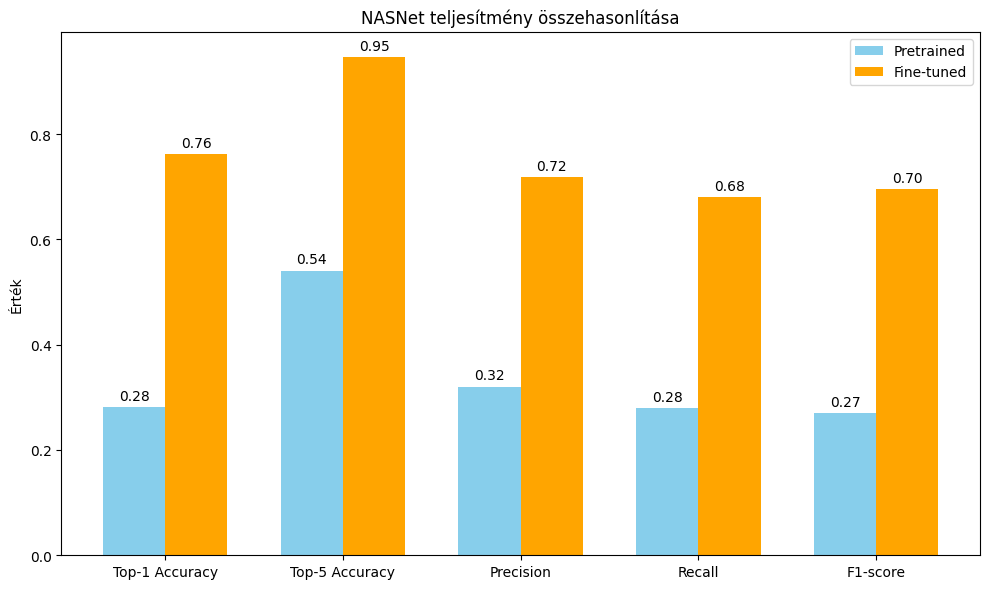
\includegraphics[width=1.0\textwidth]{images/phase02/NASNet_compare01.png}
    \caption{NASNet eredményeinek összehasonlítása}
    \label{fig:NASNet_compare01}
  \end{figure}

\subsubsection{NASNet eredményeinek összehasonlítása}
  \begin{figure}[H]
    \centering
    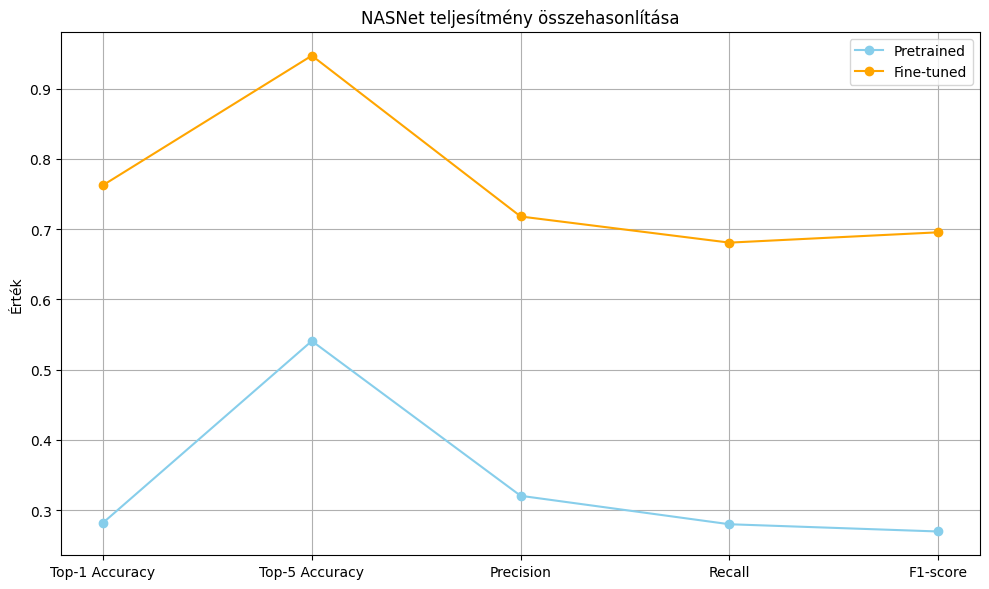
\includegraphics[width=1.0\textwidth]{images/phase02/NASNet_compare02.png}
    \caption{NASNet eredményeinek összehasonlítása}
    \label{fig:NASNet_compare02}
  \end{figure}

  \subsubsection{NASNet teljes tanítás utáni normalizált Confusion Mátrix}
  \begin{figure}[H]
    \centering
    
\includegraphics[width=0.8\textwidth]{images/phase02/NASNet_normalised_conf_mat.png}
    \caption{NASNet teljes tanítás utáni normalizált Confusion Mátrix}
    \label{fig:phase02_NASNet_normalised_conf_mat}
  \end{figure}

  \subsubsection{NASNet normalizált Confusion Mátrixok összehasonlítása}
  \begin{figure}[H]
    \centering
    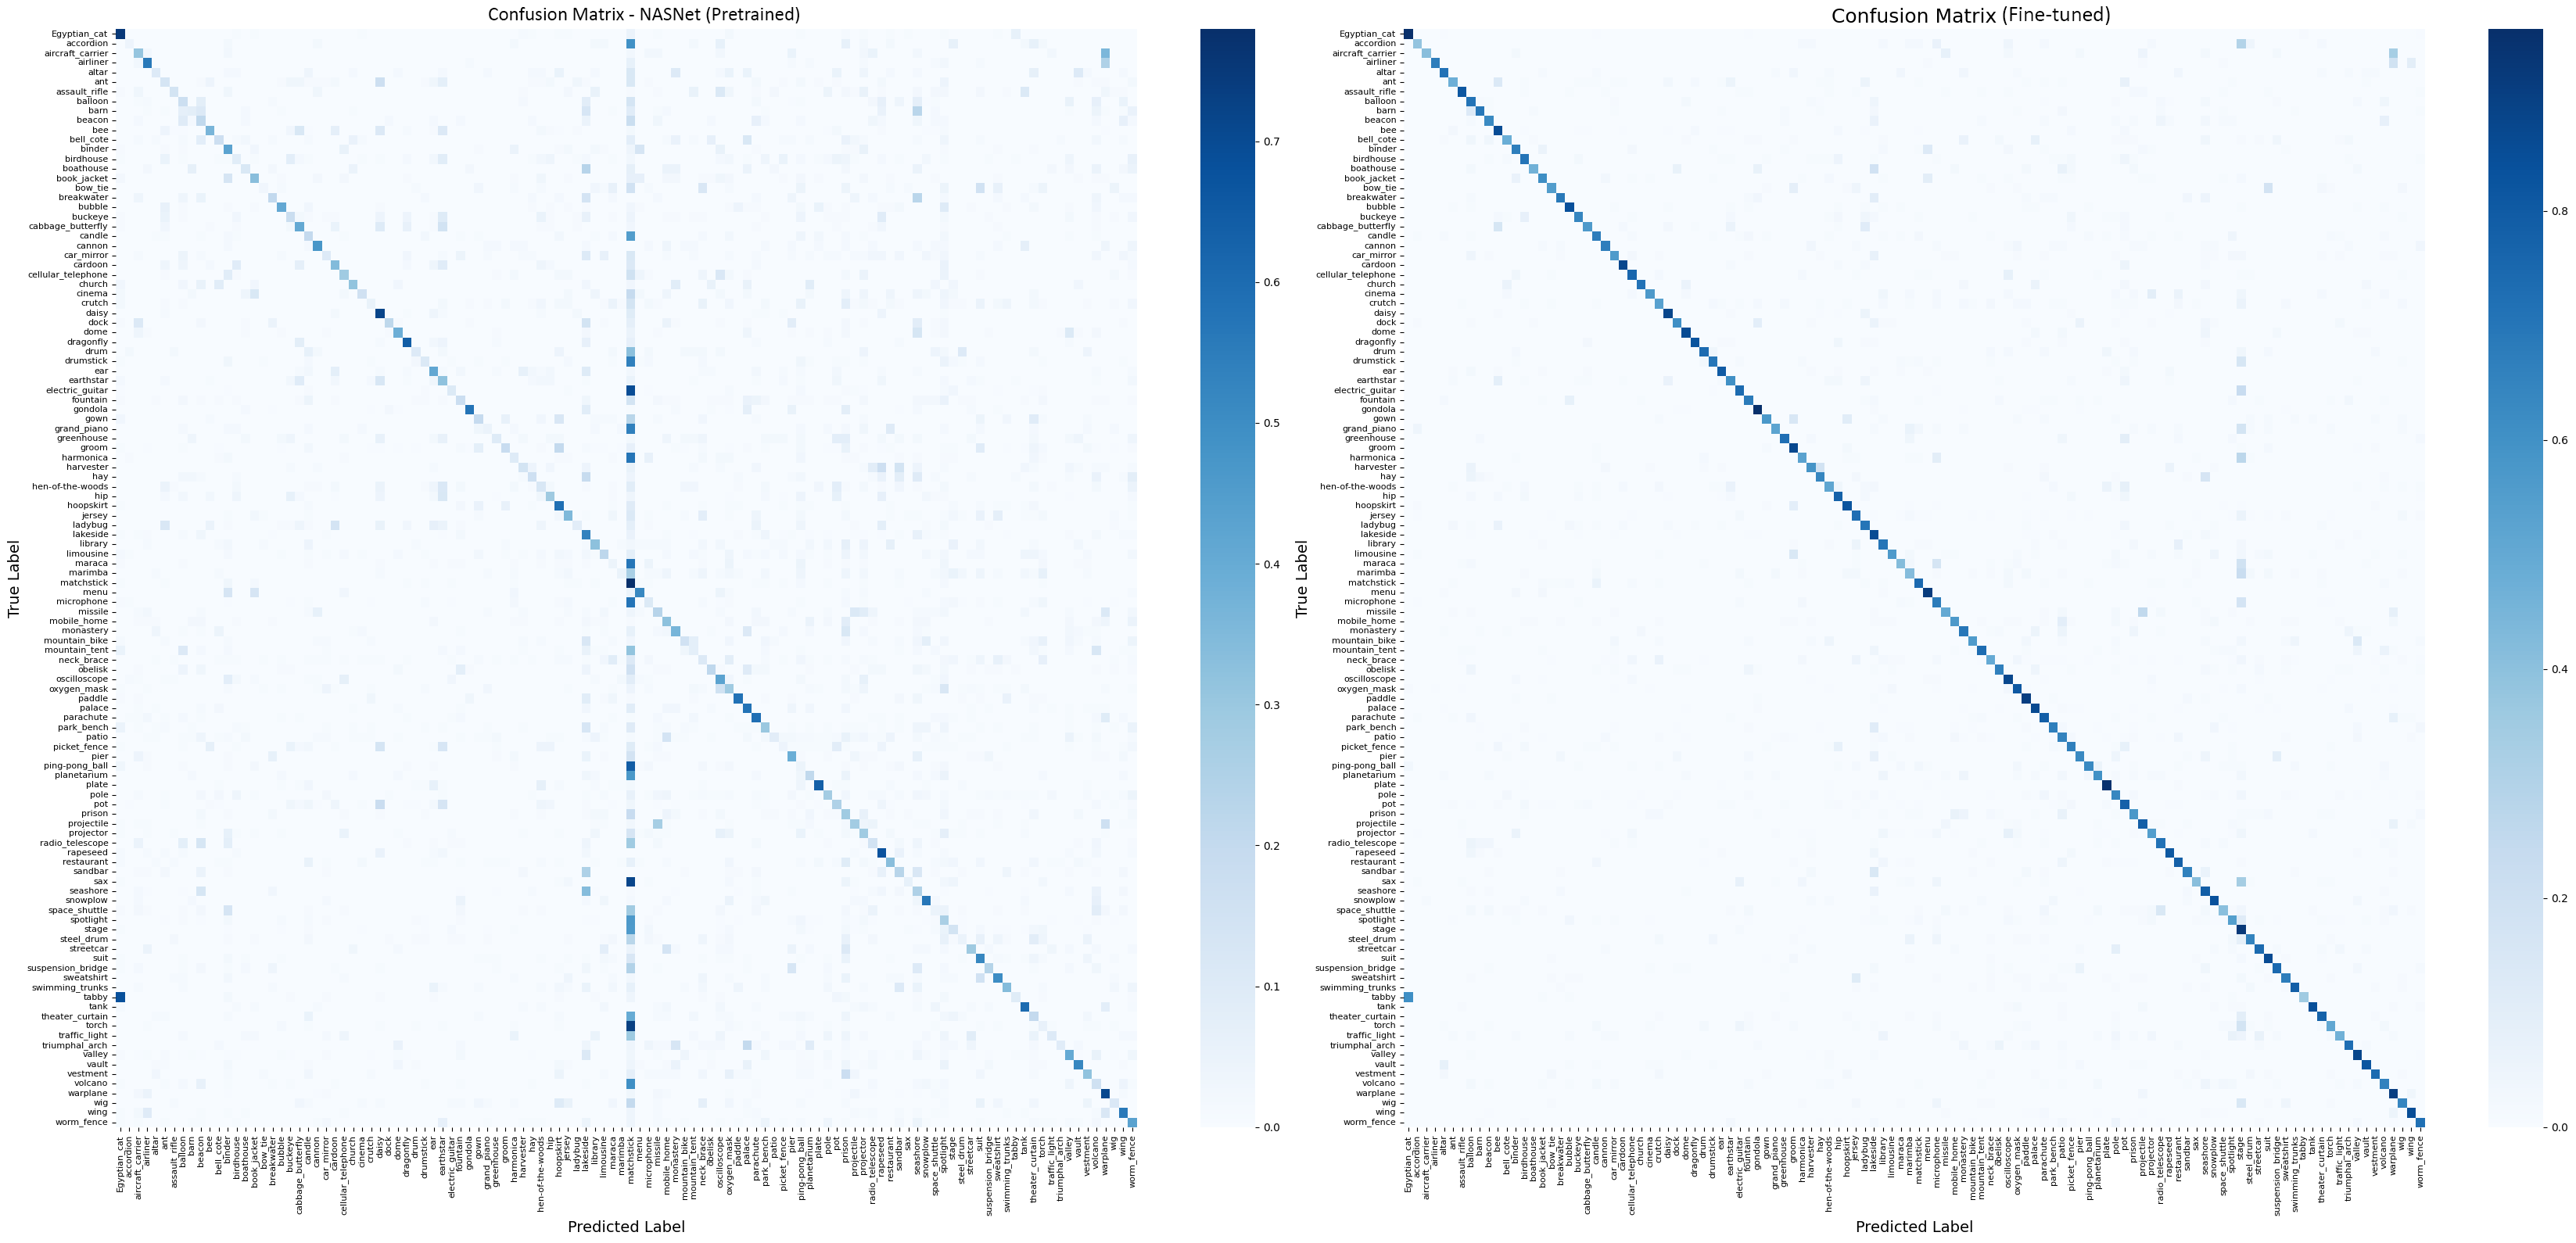
\includegraphics[width=1.0\textwidth]{images/phase02/NASNet_normalised_conf_mat_compare.png}
    \caption{NASNet normalizált Confusion Mátrixok összehasonlítása}
    \label{fig:phase02_NASNet_normalised_conf_mat_compare}
  \end{figure}


\section{Összefoglaló}

Ebben a fázisban a hét ismert modellt teszteltem úgy, hogy a 180750 képből álló sb-photothemes180k ImageNet1k cimkék szerint címkézett adathalmazon tanítottam, ahol 114 kategória van ebben a második vizsgálati fázisban a 144000 kategorizált tanító és 18000 validáló kép segítségével végeztem teljes tanítást 10 epoch-on keresztül, majd a 18000 képet tartalmazó teszt halmazon teszteltem le a modelleket ugyanazon amin az első fázisban a tanítás nélküli teszteket is végeztem. 

\subsection{Összefoglaló táblázat a második fázis mért értékeiről.}
    \begin{center}
        \begin{longtable}{lllllll}
        \caption{Összefoglaló táblázat a második fázis mért értékeiről}\label{tab:phase2_summary_table_01}\\
        \toprule
        Modell & Top-1 & Top-5 & Precision & Recall & F1 & Time(s) \\
        \midrule
        \endfirsthead
        \toprule
        Modell & Top-1 & Top-5 & Precision & Recall & F1 & Time(s) \\
        \midrule
        \endhead
        NASNet & 0.7626 & 0.9470 & 0.7180 & 0.6875 & 0.6955 & 25.11 \\
        ConvNeXt-Tiny & 0.7624 & 0.9357 & 0.7168 & 0.6841 & 0.6947 & 25.67 \\
        EfficientNet-B0 & 0.7649 & 0.9421 & 0.7130 & 0.6950 & 0.7001 & 25.26 \\
        ResNet50 & 0.7553 & 0.9351 & 0.7110 & 0.6808 & 0.6908 & 25.11 \\
        Inception-v3 & 0.7518 & 0.9320 & 0.6963 & 0.6787 & 0.6908 & 25.11 \\
        ViT-B/16 & 0.7414 & 0.9257 & 0.6935 & 0.6636 & 0.6730 & 42.40 \\
        DenseNet121 & 0.7400 & 0.9266 & 0.6811 & 0.6808 & 0.6696 & 25.23 \\
        \bottomrule
        \end{longtable}
    \end{center}

\subsection{Top 1 pontosságok összehasonlítása teljes tanítás után.}
    \begin{figure}[H]
        \centering
        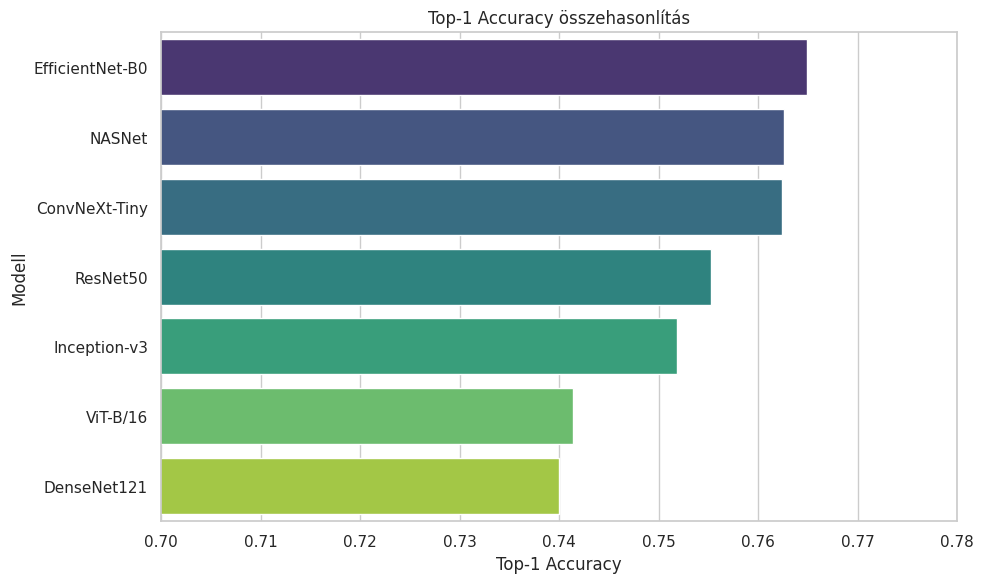
\includegraphics[width=1.0\textwidth]{images/phase02/phase02_summary_top1.png}
        \caption{Top 1 pontosságok összehasonlítása teljes tanítás után.}
        \label{fig:phase02_summary_top1}
    \end{figure}

\subsection{F1 értékek összehasonlítása teljes tanítás után.}
    \begin{figure}[H]
        \centering
        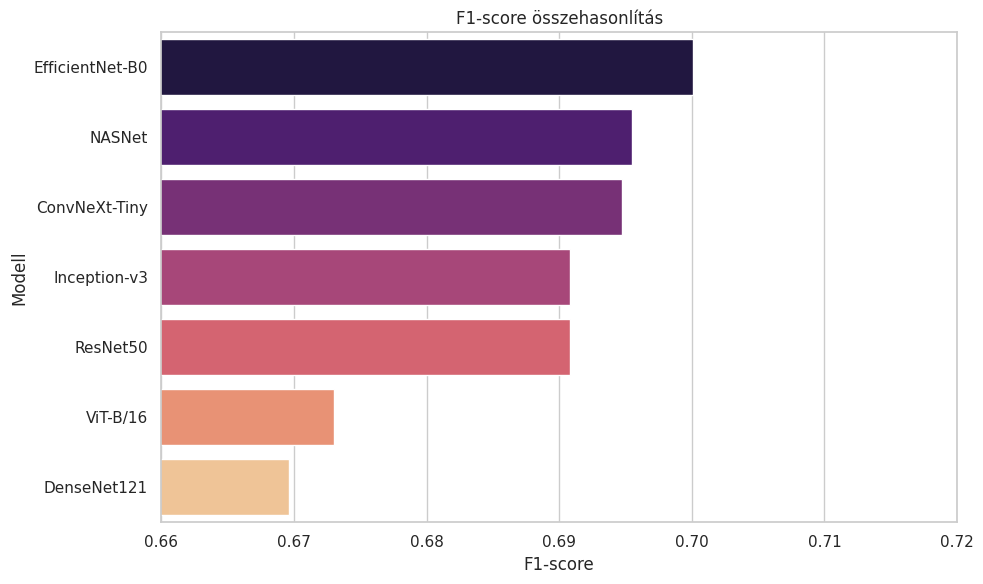
\includegraphics[width=1.0\textwidth]{images/phase02/phase02_summary_f1.png}
        \caption{F1 értékek összehasonlítása teljes tanítás után.}
        \label{fig:phase02_summary_top1}
    \end{figure}

\subsection{Futási idők összehasonlítása teljes tanítás után a teszt halmazon.}
    \begin{figure}[H]
        \centering
        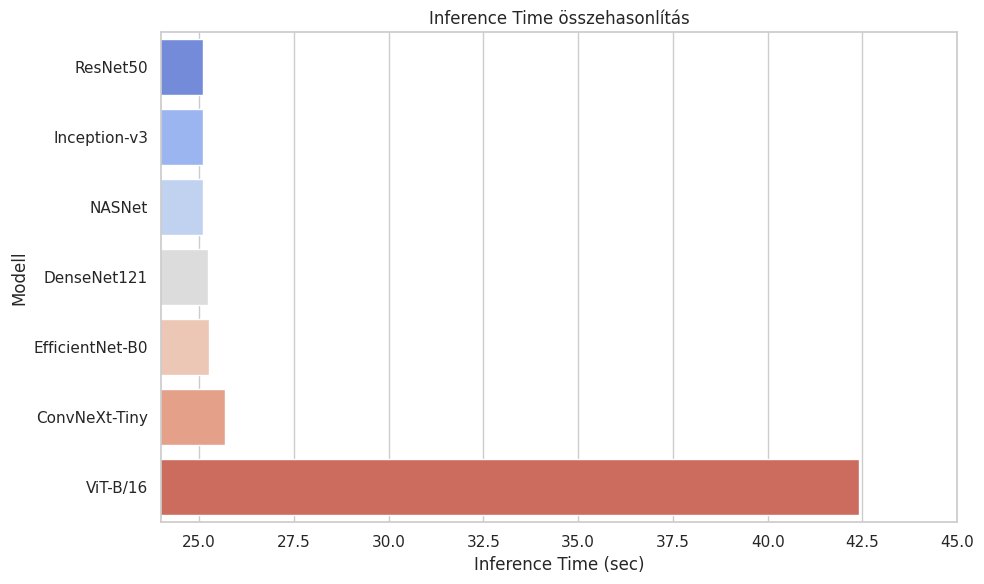
\includegraphics[width=1.0\textwidth]{images/phase02/phase02_summary_time.png}
        \caption{Futási idők összehasonlítása teljes tanítás után a teszt halmazon.}
        \label{fig:phase02_summary_time}
    \end{figure}

\subsection{Top 1 és Top 5 pontosságok összehasonlítása teljes tanítás után a teszt halmazon.}
    \begin{figure}[H]
        \centering
        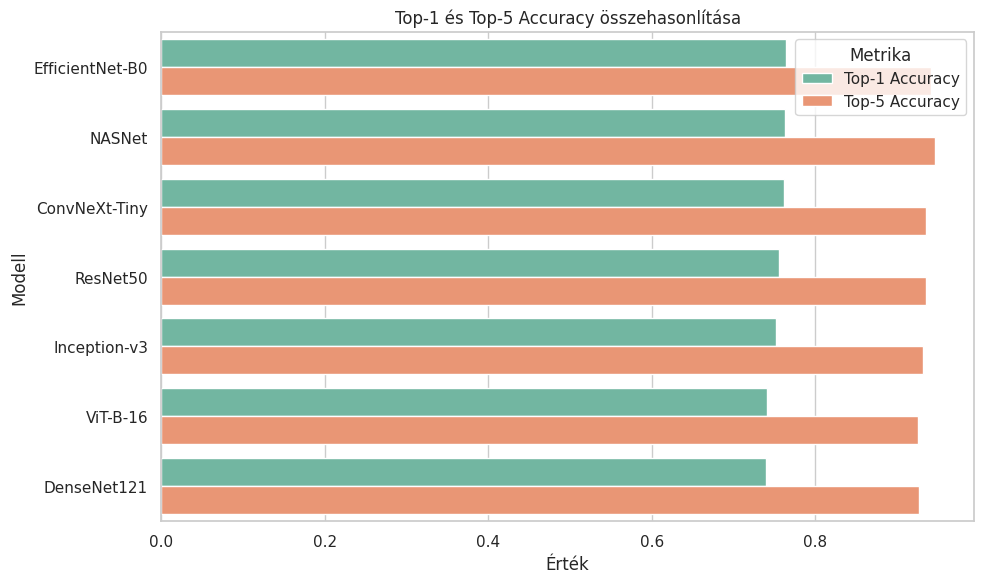
\includegraphics[width=1.0\textwidth]{images/phase02/phase02_summary_top1vstop5.png}
        \caption{Top 1 és Top 5 pontosságok összehasonlítása teljes tanítás után a teszt halmazon.}
        \label{fig:phase02_summary_top1vstop5}
    \end{figure}

\subsection{Precision, Recall és F1 összehasonlítása teljes tanítás után a teszt halmazon.}
    \begin{figure}[H]
        \centering
        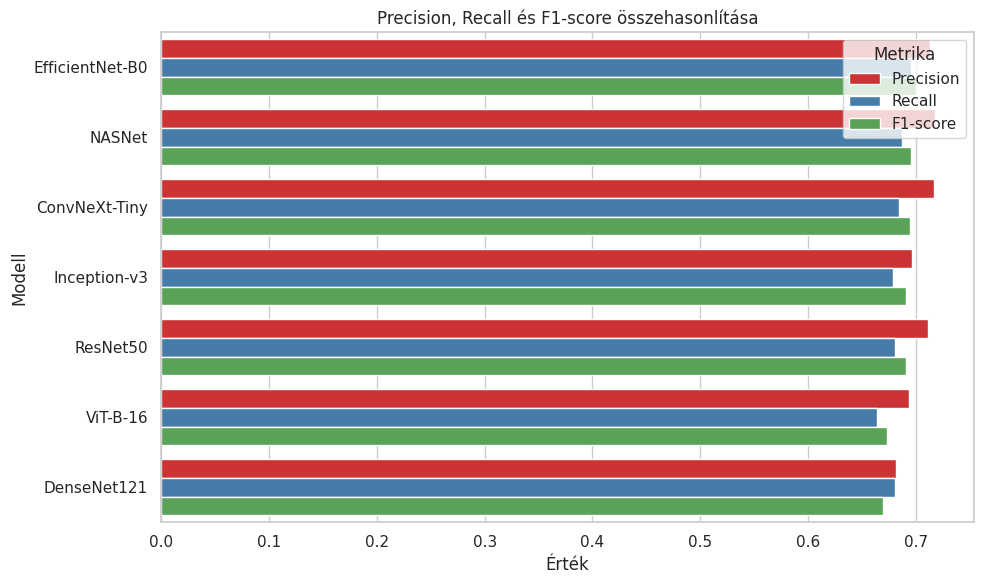
\includegraphics[width=1.0\textwidth]{images/phase02/phase02_summary_prec_rec_f1.png}
        \caption{Precision, Recall és F1 összehasonlítása teljes tanítás után a teszt halmazon.}
        \label{fig:phase02_summary_prec_rec_f1}
    \end{figure}

\subsection{Összehasonlító táblázat az első és a második fázis mért értékeiről.}
    \begin{center}
        \begin{longtable}{lllll}
        \caption{Összehasonlító táblázat az első és a második fázis mért értékeiről – Alapvető metrikák}\label{tab:phase2_summary_table_02_basic}\\
        \toprule
        Modell & Top-1 (PT) & Top-1 (FT) & Top-5 (PT) & Top-5 (FT) \\
        \midrule
        \endfirsthead
        \toprule
        Modell & Top-1 (PT) & Top-1 (FT) & Top-5 (PT) & Top-5 (FT) \\
        \midrule
        \endhead
        ConvNeXt-Tiny & 0.5048 & 0.7624 & 0.8471 & 0.9357 \\
        EfficientNet-B0 & 0.4802 & 0.7649 & 0.8217 & 0.9421 \\
        ResNet50 & 0.4698 & 0.7553 & 0.7962 & 0.9351 \\
        Inception-v3 & 0.4763 & 0.7518 & 0.8008 & 0.9320 \\
        ViT-B-16 & 0.5308 & 0.7414 & 0.8582 & 0.9257 \\
        DenseNet121 & 0.4498 & 0.7400 & 0.7806 & 0.9266 \\
        \bottomrule
        \end{longtable}
    \end{center}
    

    \begin{center}
        \begin{longtable}{lllll}
        \caption{Összehasonlító táblázat az első és a második fázis mért értékeiről – Pontosság és visszahívás}\label{tab:phase2_summary_table_02_precision_recall}\\
        \toprule
        Modell & Precision (PT) & Precision (FT) & Recall (PT) & Recall (FT) \\
        \midrule
        \endfirsthead
        \toprule
        Modell & Precision (PT) & Precision (FT) & Recall (PT) & Recall (FT) \\
        \midrule
        \endhead
        ConvNeXt-Tiny & 0.4917 & 0.7168 & 0.4369 & 0.6841 \\
        EfficientNet-B0 & 0.4137 & 0.7130 & 0.4039 & 0.6950 \\
        ResNet50 & 0.3934 & 0.7110 & 0.3797 & 0.6808 \\
        Inception-v3 & 0.3833 & 0.6963 & 0.3896 & 0.6787 \\
        ViT-B-16 & 0.4629 & 0.6935 & 0.4419 & 0.6636 \\
        DenseNet121 & 0.3874 & 0.6811 & 0.3611 & 0.6680 \\
        \bottomrule
        \end{longtable}
    \end{center}
        

    \begin{center}
        \begin{longtable}{lllll}
        \caption{Összehasonlító táblázat az első és a második fázis mért értékeiről – F1 és idő}\label{tab:phase2_summary_table_02_f1_time}\\
        \toprule
        Modell & F1 (PT) & F1 (FT) & Time (PT) & Time (FT) \\
        \midrule
        \endfirsthead
        \toprule
        Modell & F1 (PT) & F1 (FT) & Time (PT) & Time (FT) \\
        \midrule
        \endhead
        ConvNeXt-Tiny & 0.4194 & 0.6947 & 38.40s & 25.67s \\
        EfficientNet-B0 & 0.3829 & 0.7001 & 28.89s & 25.26s \\
        ResNet50 & 0.3592 & 0.6908 & 25.21s & 25.11s \\
        Inception-v3 & 0.3683 & 0.6827 & 38.06s & 33.62s \\
        ViT-B-16 & 0.4307 & 0.6908 & 92.13s & 42.40s \\
        DenseNet121 & 0.3408 & 0.6696 & 25.15s & 25.23s \\
        \bottomrule
        \end{longtable}
    \end{center}

    \subsection{Top 1 és Top 5 pontosság összehasonlítása Pretrained és a Finetuned mérések között.}
    \begin{figure}[H]
        \centering
        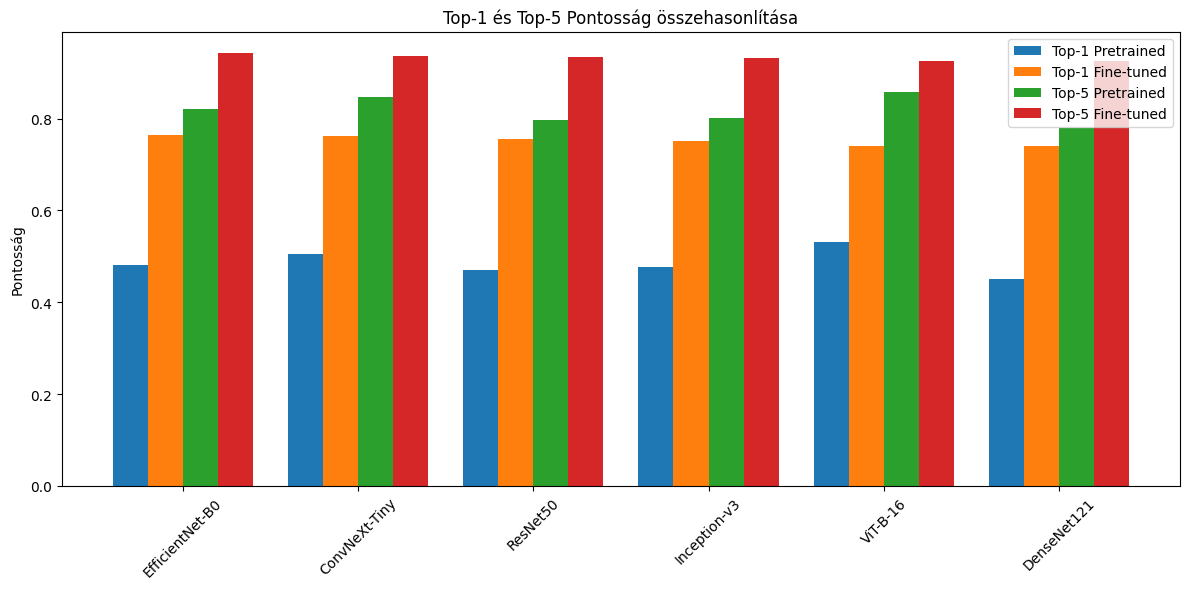
\includegraphics[width=1.0\textwidth]{images/phase02/phase02_summary_top1_vs_top5_pre_vs_fine.png}
        \caption{Top 1 és Top 5 pontosság összehasonlítása Pretrained és a Finetuned mérések között.}
        \label{fig:phase02_summary_top1_vs_top5_pre_vs_fine}
    \end{figure}

\subsection{Precision és Recall összehasonlítása Pretrained és a Finetuned mérések között.}
    \begin{figure}[H]
        \centering
        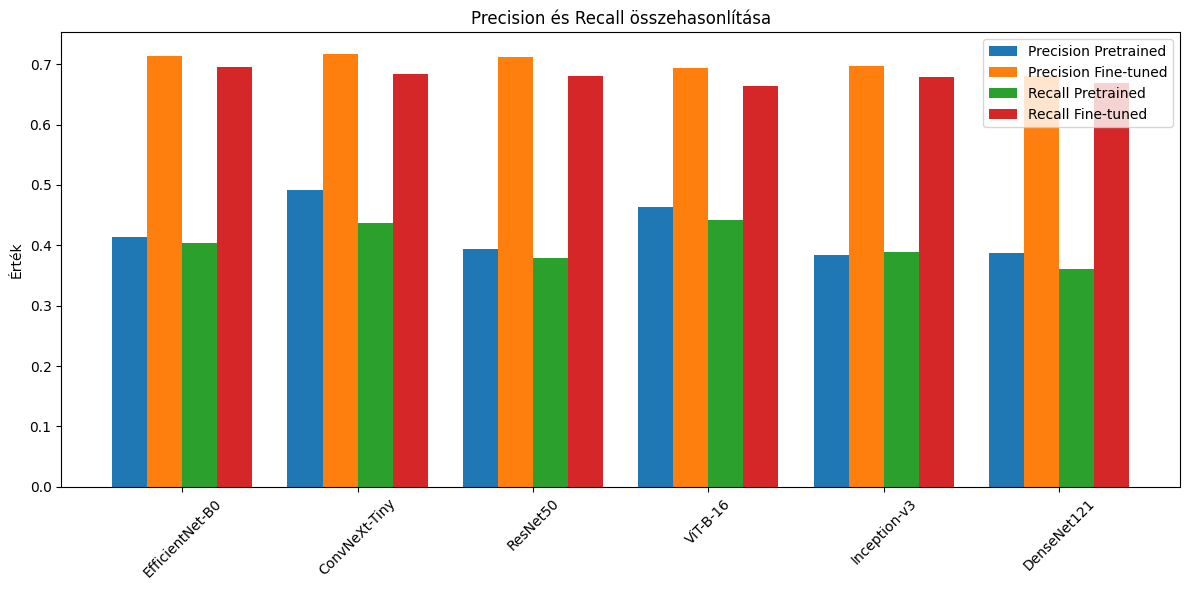
\includegraphics[width=1.0\textwidth]{images/phase02/phase02_summary_prec_vs_rec_pre_vs_fine.png}
        \caption{Precision és Recall összehasonlítása Pretrained és a Finetuned mérések között.}
        \label{fig:phase02_summary_prec_vs_rec_pre_vs_fine}
    \end{figure}

\subsection{F1 score összehasonlítása Pretrained és a Finetuned mérések között.}
    \begin{figure}[H]
        \centering
        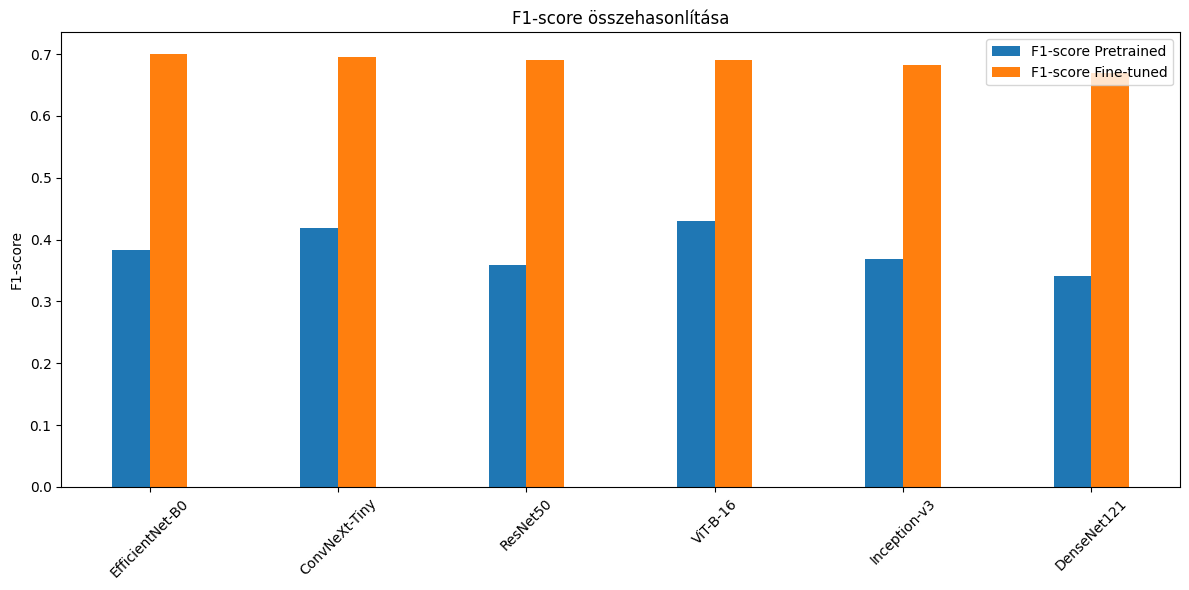
\includegraphics[width=1.0\textwidth]{images/phase02/phase02_summary_F1_pre_vs_fine.png}
        \caption{F1 score összehasonlítása Pretrained és a Finetuned mérések között.}
        \label{fig:phase02_summary_F1_pre_vs_fine}
    \end{figure}

\subsection{A Precision és a Fine-tuned modellek értékelése}
    A fenti eredmények alapján megállapítható, hogy a finomhangolt (fine-tuned) modellek jelentős teljesítményjavulást mutatnak a kiindulási, előképzett (pretrained) állapothoz képest. Különösen az EfficientNet-B0 és a ConvNeXt-Tiny modellek emelkednek ki, amelyek a legmagasabb Top-1 és Top-5 pontosságot érték el a finomhangolás után.

    A Precision, Recall és F1-score metrikák szintén javulást mutatnak minden modell esetében a finomhangolás hatására. Ez arra utal, hogy a modellek nemcsak pontosabbak lettek, hanem jobban képesek felismerni a releváns jellemzőket az adathalmazon.

    Az inference idő tekintetében a ViT-B-16 modell jelentősen hosszabb időt igényel

\subsection{Tanítási ciklusok elemzése}
Általános megfigyelések:
Tanítási pontosságban (Train Accuracy) ResNet50 (96.51\%) és ConvNeXt-Tiny (95.77\%) szerepeltek kiemelkedően.
Validációs pontosságban (Validation Accuracy) az EfficientNet-B0 (76.58\%) és NASNet (75.98\%) mutatták a legjobb eredményt.
A legtöbb modellnél overfitting (túlilleszkedés) jelentkezett: a Train Loss nagyon lecsökkent, miközben a Val Loss magas maradt (1 körül vagy felette).
NASNet csak 3 epoch alatt futott, mégis a legjobb vagy közel legjobb validációs eredményt érte el, ami hatékony tanulásra utal.
ViT-B/16 (Vision Transformer) és Inception-v3 bár jól tanultak (magas train acc), a validációs loss alapján nem tudtak igazán generalizálni.

Modellenként:
ResNet50: 
Nagyon erős tanítási eredmény, de látványos overfitting.
DenseNet121: 
Stabil fejlődés, viszont a validációs eredmény nem nőtt jelentősen a vége felé.
EfficientNet-B0: 
Legjobb tradeoff: relatíve jó tanulás + legjobb validáció.
ConvNeXt-Tiny: 
Nagyon jól tanult, de a validáció során hullámzó teljesítményt mutatott.
ViT-B/16: 
Transformer alapú architektúra itt nem volt erősebb, mint a CNN-ek.
Inception-v3: 
Stabil, de szintén overfitting jelei.
NASNet: 
Gyors, kevés epoch alatti hatékony tanulás. Figyelemre méltóan jó validációs pontosság.

\subsection{A Train és Validation loss alakulása modellenként.}
    \begin{figure}[H]
        \centering
        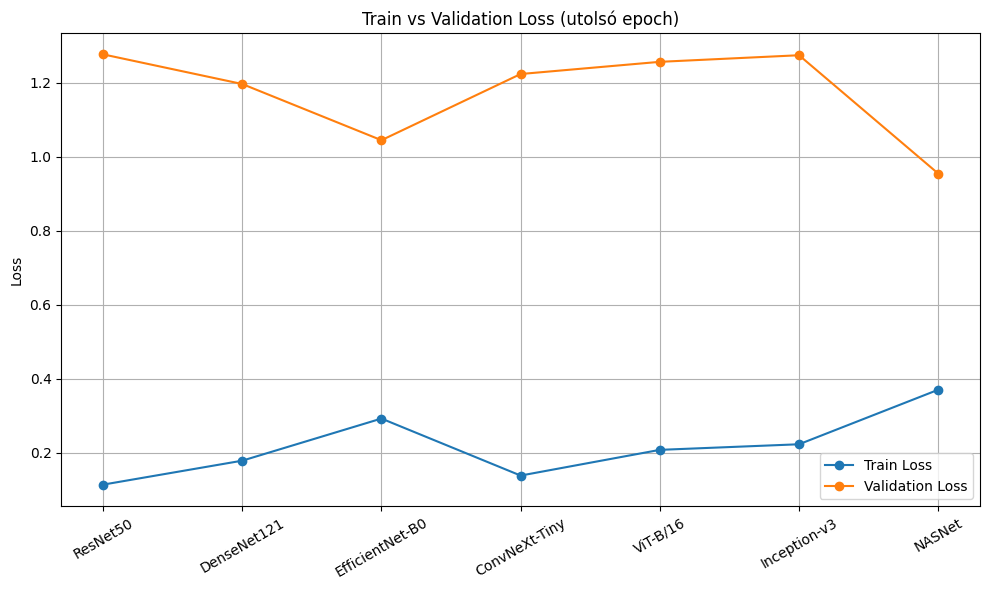
\includegraphics[width=1.0\textwidth]{images/phase02/phase2_summary_learning_stat_last_01.png}
        \caption{A Train és Validation loss alakulása modellenként.}
        \label{fig:phase2_summary_learning_stat_last_01.png}
    \end{figure}

\subsection{A Train és Validation accuracy alakulása modellenként.}
    \begin{figure}[H]
        \centering
        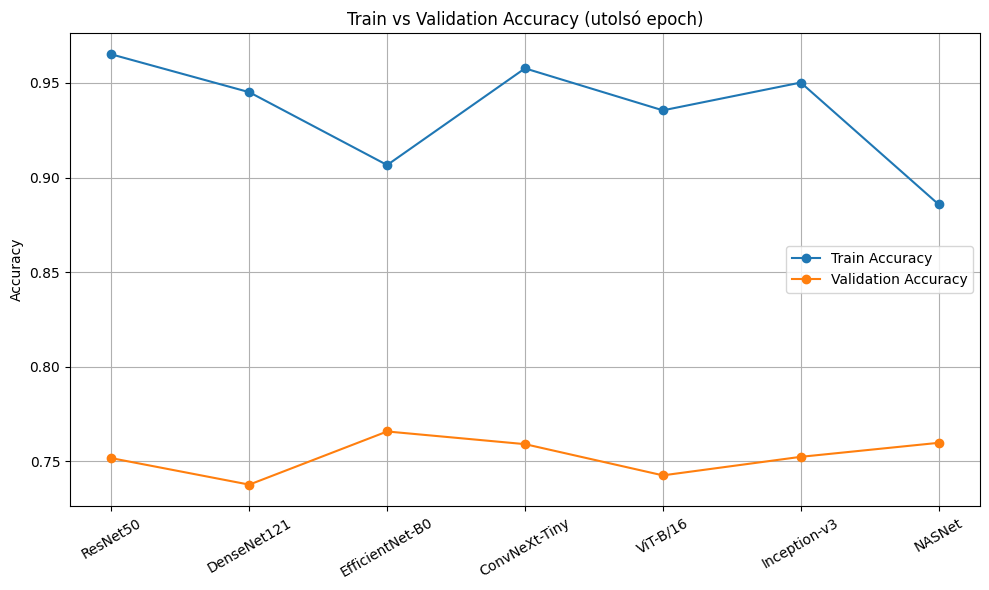
\includegraphics[width=1.0\textwidth]{images/phase02/phase2_summary_learning_stat_last_02.png}
        \caption{A Train és Validation accuracy alakulása modellenként.}
        \label{fig:phase2_summary_learning_stat_last_02.png}
    \end{figure}

\subsection{A Train és Validation loss alakulása modellenként epoch-ok szerint.}
    \begin{figure}[H]
        \centering
        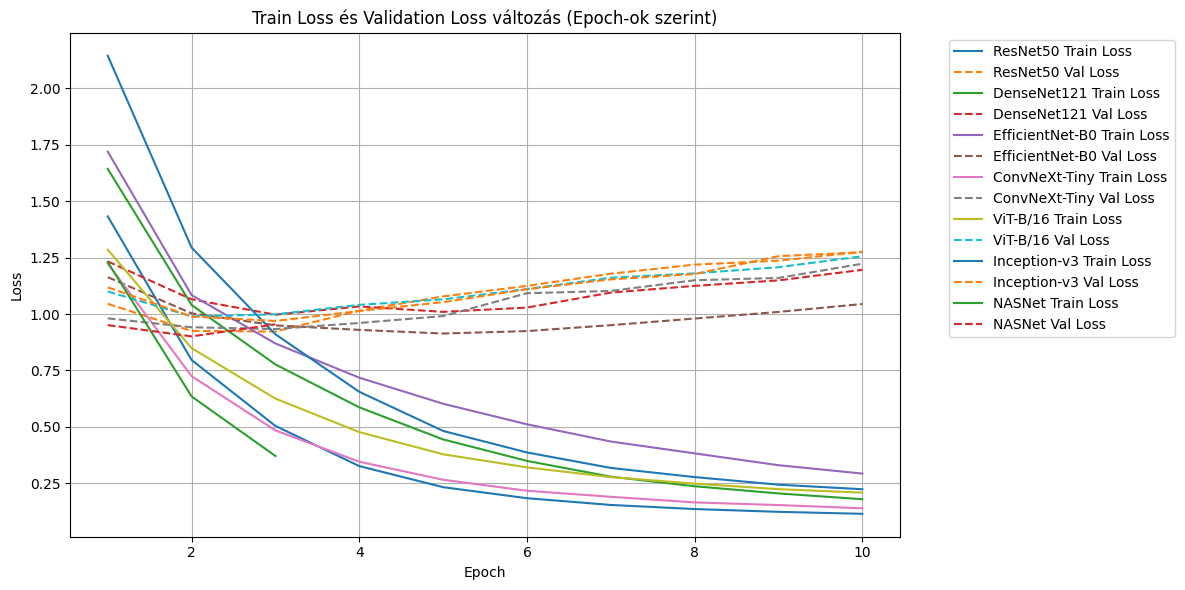
\includegraphics[width=1.0\textwidth]{images/phase02/phase2_summary_learning_stat_full_01.png}
        \caption{A Train és Validation loss alakulása modellenként epoch-ok szerint.}
        \label{fig:phase2_summary_learning_stat_last_01.png}
    \end{figure}

\subsection{A Train és Validation accuracy alakulása modellenként epoch-ok szerint.}
    \begin{figure}[H]
        \centering
        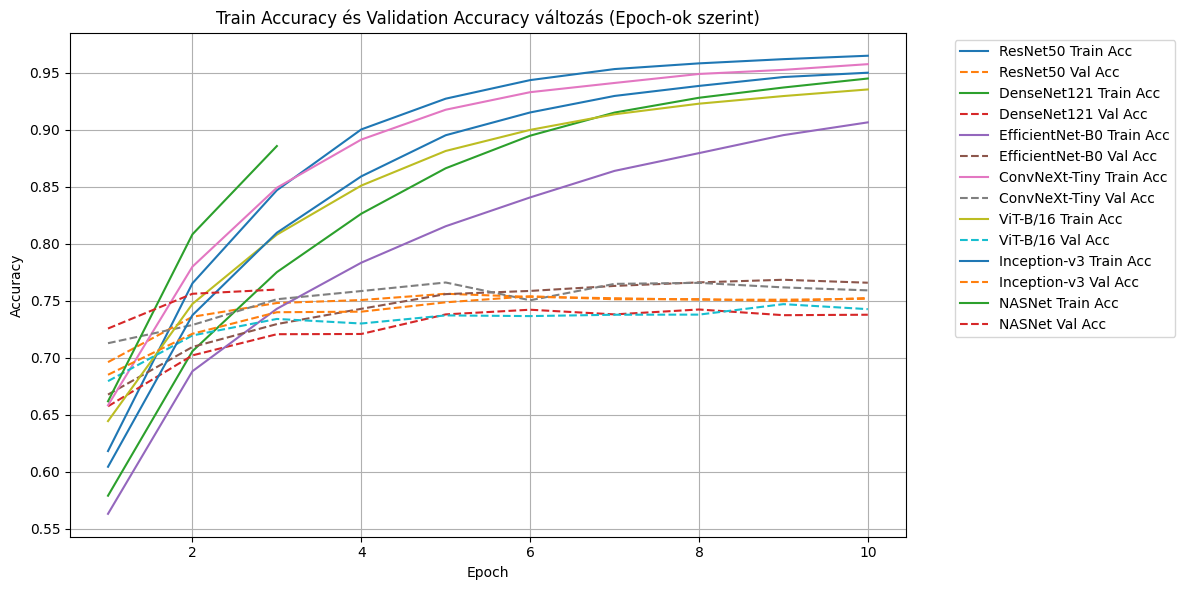
\includegraphics[width=1.0\textwidth]{images/phase02/phase2_summary_learning_stat_full_02.png}
        \caption{A Train és Validation accuracy alakulása modellenként epoch-ok szerint.}
        \label{fig:phase2_summary_learning_stat_last_02.png}
    \end{figure}

\subsection{A második fázis rövid szöveges értékelése}
    A második mérési fázis során a SBphotothemes180k [ImageNet114] adathalmazon végzett teljes tanítási folyamat után a különböző modellek teljesítményét értékeltük. Az alábbi megállapítások születtek:

    EfficientNet-B0 érte el a legmagasabb Top-1 pontosságot (76.49\%) és F1-score-t (70.01\%), miközben az inference ideje is versenyképes maradt. Ez alátámasztja az EfficientNet architektúra hatékonyságát és pontosságát, különösen a korlátozott erőforrásokkal rendelkező környezetekben.

    NASNet kiemelkedett a Top-5 pontosság terén (94.70\%) és a legmagasabb precizitást (71.80\%) érte el, ami a modell mély és összetett architektúrájának köszönhető. Azonban az inference ideje megegyezett más modellekével, ami azt jelzi, hogy a komplexitás nem feltétlenül jár együtt hosszabb feldolgozási idővel.

    ConvNeXt-Tiny és ResNet50 modellek kiegyensúlyozott teljesítményt mutattak, mind a pontosság, mind az inference idő tekintetében. Ez teszi őket megbízható választássá általános célú alkalmazásokhoz.

    ViT-B/16, bár transformer alapú modellként ígéretes, a jelenlegi adathalmazon nem tudta felülmúlni a CNN alapú modelleket. Az inference ideje is jelentősen hosszabb volt, ami korlátozhatja a valós idejű alkalmazásokban való használatát.

    Inception-v3 stabil teljesítményt nyújtott, különösen az F1-score (69.08\%) és az inference idő (25.11 sec) tekintetében, ami a modell érettségét és optimalizáltságát tükrözi.

    DenseNet121 hasonlóan jó eredményeket ért el, különösen a recall értékben (68.08\%), ami a modell hatékony információáramlását és mély kapcsolatokat kihasználó architektúráját mutatja.

    Összefoglalva, a teljes tanítási folyamat jelentős javulást eredményezett minden modell esetében a tanítás nélküli állapothoz képest. Az eredmények alapján az EfficientNet-B0 és a NASNet modellek kiemelkednek a pontosság és hatékonyság terén, míg a ConvNeXt-Tiny és a ResNet50 modellek megbízható és kiegyensúlyozott teljesítményt nyújtanak. A választás során figyelembe kell venni az alkalmazás specifikus igényeit, beleértve a pontosságot, a feldolgozási időt és az erőforrás-korlátokat.


\chapter{III. Fázis: Iteratív tanítás}

    \section{ResNet50}

    \section{DenseNet121}

    \section{EfficientNet-B0}

    \section{ConvNeXt-Tiny}

    \section{ViT-B/16}

    \section{Inception-v3}

    \section{NASNet}
    
    \section{Összefoglaló}


\chapter{IV. Fázis: Saját modell fejlesztése}

A méréssorozat negyedik fázisában egy egyedileg kialakított neurális háló kifejlesztésére és kiértékelésére került sor. A cél olyan modell létrehozása volt, amely a nagy, erőforrás-igényes hálózatok (pl. ViT, ConvNeXt, EfficientNet) pontosságát megközelíti, de lényegesen kisebb számítási igény mellett. Ez lehetővé teszi a modell lokális, valós idejű, alacsony költségű alkalmazását is.

A fejlesztés alapját a jól bevált \textbf{ResNet18} architektúra képezte, amely megfelelő egyensúlyt nyújt a taníthatóság és a teljesítmény között. A modell \texttt{backbone} része változatlan maradt, míg az utolsó teljesen összekapcsolt (fully-connected) réteg helyére különféle saját fejrészek (head-ek) kerültek.

A következőkben részletesen bemutatjuk az alkalmazott ResNet18 modellt, valamint a négy vizsgált fejváltozatot: \textbf{Baseline, Deep, Hybrid-v1, Hybrid-v2}.

\section{A ResNet18 ismertetése}
A személyes kötődés miatt választottam ezt a modellt. Ez volt az első amivel az egyetemen dolgoztam, így jól ismerem.
A ResNet18 az egyik legismertebb és legszélesebb körben alkalmazott konvolúciós neurális hálózat, melyet a \textit{Microsoft Research} fejlesztett ki. A modell fő innovációja a \textbf{residual connection} használata, amely lehetővé teszi a mély hálók hatékony tanítását a gradiens-visszaterjedés során fellépő problémák enyhítésével.

A ResNet18 a következő fő komponensekből áll:
\begin{itemize}
  \item Kezdeti konvolúciós réteg + batch normalizáció + max pooling
  \item Négy egymásra épülő blokk (2-2 residual egységgel)
  \item Átlagos leképezés (global average pooling)
  \item Fully connected kimeneti réteg (ez került eltávolításra a vizsgálathoz)
\end{itemize}

A \texttt{fc} és \texttt{avgpool} rétegek helyére került be az egyedileg tervezett fejrészek egyike.

\section{A Baseline fej ismertetése}

A Baseline fej a legegyszerűbb, mégis hatékony megoldás. Lényege egy kétlépcsős, lineáris osztályozó blokk, amely gyors konvergenciát és stabil tanulást biztosít, különösen kis méretű adathalmazokon. Ez a fej alacsony paraméterszámú és kevéssé túlilleszkedésre hajlamos, ezért kiváló kiindulópontként szolgált.

\begin{verbatim}
nn.Sequential(
    nn.Linear(in_features, 256),
    nn.ReLU(),
    nn.Dropout(0.3),
    nn.Linear(256, num_classes)
)
\end{verbatim}

A Dropout alkalmazása segít a generalizációs képesség javításában, míg a ReLU aktiváció gyors tanulást tesz lehetővé.

\section{A Deep fej ismertetése}

A Deep fej mélyebb, háromrétegű architektúra, amely nagyobb reprezentációs kapacitással bír. Célja a tanulási képesség növelése mélyebb jellemzők segítségével, különösen bonyolultabb osztályok esetén.

\begin{verbatim}
nn.Sequential(
    nn.Linear(in_features, 512),
    nn.ReLU(),
    nn.Dropout(0.3),
    nn.Linear(512, 256),
    nn.ReLU(),
    nn.Dropout(0.3),
    nn.Linear(256, num_classes)
)
\end{verbatim}

Ez a fejváltozat kifejezetten akkor bizonyult előnyösnek, ha nagyobb adathalmazon (pl. 25k train minta) történik a tanítás, mivel képes mélyebb döntési határokat megtanulni.

\section{A Hybrid-v1 fej ismertetése}

A Hybrid-v1 fej egy újszerű megközelítést alkalmaz: a ResNet18 utolsó konvolúciós kimenetére egy 1x1-es konvolúciós réteg kerül, amely lekicsinyíti a csatornaszámot. Ezután jön egy adaptív átlagolás, normalizálás és egy nemlineáris aktiváció (GELU). A végeredményt egy teljesen összekapcsolt réteg végzi el.

\begin{verbatim}
nn.Sequential(
    nn.Conv2d(512, 256, kernel_size=1),
    nn.AdaptiveAvgPool2d((1, 1)),
    nn.LayerNorm([256, 1, 1]),
    nn.GELU(),
    nn.Flatten(),
    nn.Linear(256, num_classes)
)
\end{verbatim}

A LayerNorm javítja a tanítási stabilitást, míg a GELU finomabb nemlinearitást biztosít. Ez a fejváltozat nagyon jó egyensúlyt mutatott a teljesítmény és a számítási igény között.

\section{A Hybrid-v2 fej ismertetése}

A Hybrid-v2 fej a v1 továbbfejlesztett változata. Itt a 1x1-es konvolúciót lecseréltük két egymásra épülő, klasszikus 3x3-as konvolúciós blokkra (BatchNorm + GELU aktivációval), így a fej mélyebb, de még mindig könnyen tanítható maradt.

\begin{verbatim}
nn.Sequential(
    nn.Conv2d(512, 256, kernel_size=3, padding=1),
    nn.BatchNorm2d(256),
    nn.GELU(),
    nn.Conv2d(256, 128, kernel_size=3, padding=1),
    nn.BatchNorm2d(128),
    nn.GELU(),
    nn.AdaptiveAvgPool2d((1, 1)),
    nn.Flatten(),
    nn.Linear(128, num_classes)
)
\end{verbatim}

Ez a kialakítás a legjobb teljesítményt nyújtotta a saját modellek között, miközben továbbra is gyorsan futott és jól skálázódott GPU-n és akár CPU-n is.

\bigskip

Mind a négy fej logikusan kapcsolódott a ResNet18 backbone-hoz, és jól illeszkedett a projekt céljához: egy könnyű, de pontos modell kifejlesztéséhez. A fázis eredményei azt mutatták, hogy megfelelő architektúra választásával a mély modellek pontosságát akár egy ResNet18-alapú saját háló is megközelítheti.


    \section{Mérések}

        \subsection{I. Fázis: Tanítás nélküli tesztelés}

        \subsection{II. Fázis: Teljes tanítás}

        \subsection{III. Fázis: Iteratív tanítás}
        
    \section{Összefoglalás}

\chapter{Legfontosabb eredmények}
Ebben a zárófejezetben a teljesség igénye nélkül megismétlem a legfontosabb mérési eredményeket a négy fázisból és ezeket elemzem szövegesen a teljes kép érdekében.

\section{Következtetések tanítás nélküli tesztek után kapott eredményekből.}

    \subsubsection{Összehasonlító Top-1 és Top-5 diagram a tanítás nélküli tesztekről.}
    \begin{figure}[H]
    \centering
    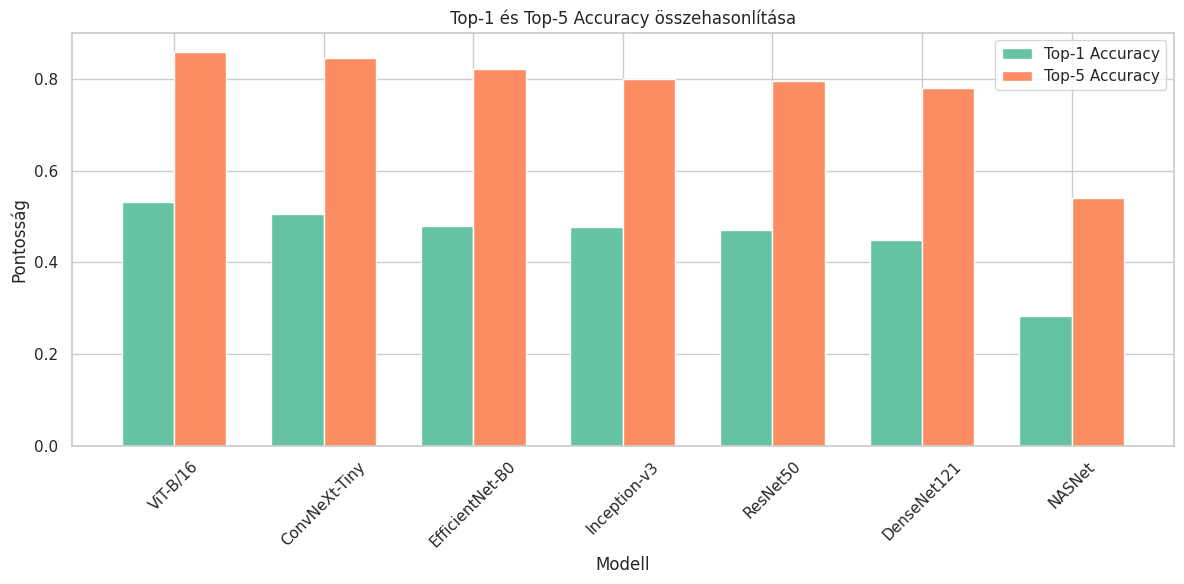
\includegraphics[width=1.0\textwidth]{images/phase01/summary01.png}
    \caption{sszehasonlító Top-1 és Top-5 diagram a tanítás nélküli tesztekről.}
    \label{fig:top1zop5phase12}
    \end{figure}

    \subsubsection{Összehasonlító Precision, Recall, F1 diagram a tanítás nélküli tesztekről.}
    \begin{figure}[H]
    \centering
    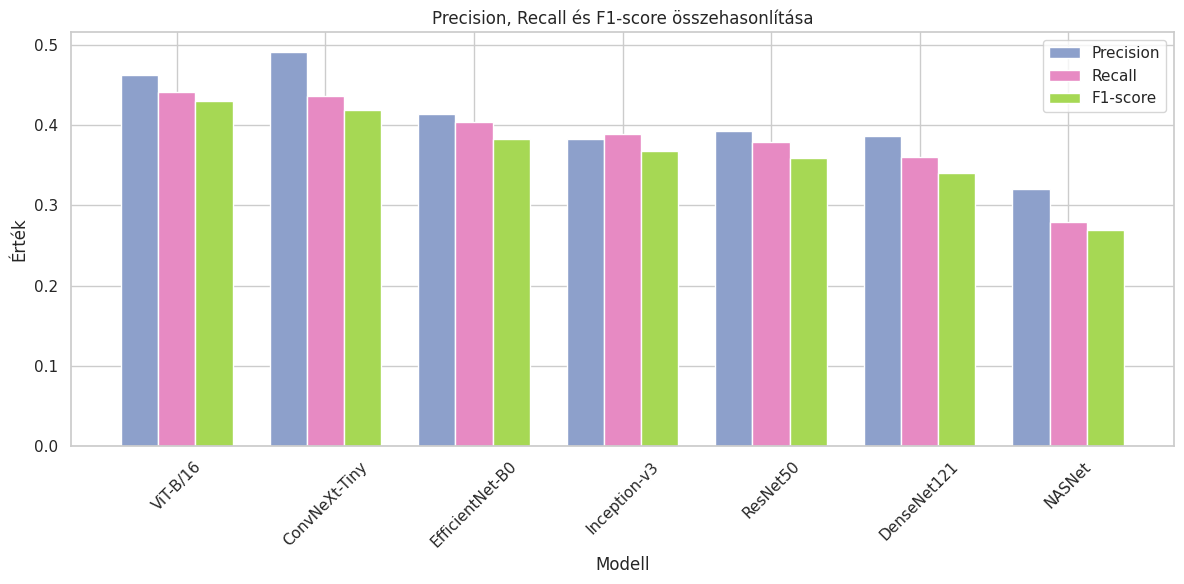
\includegraphics[width=0.75\textwidth]{images/phase01/summary02.png}
    \caption{sszehasonlító Precision, Recall, F1 diagram a tanítás nélküli tesztekről.}
    \label{fig:top1zop5phase1}
    \end{figure}

    \subsubsection{Összehasonlító idő diagram a tanítás nélküli tesztekről.}
    \begin{figure}[H]
    \centering
    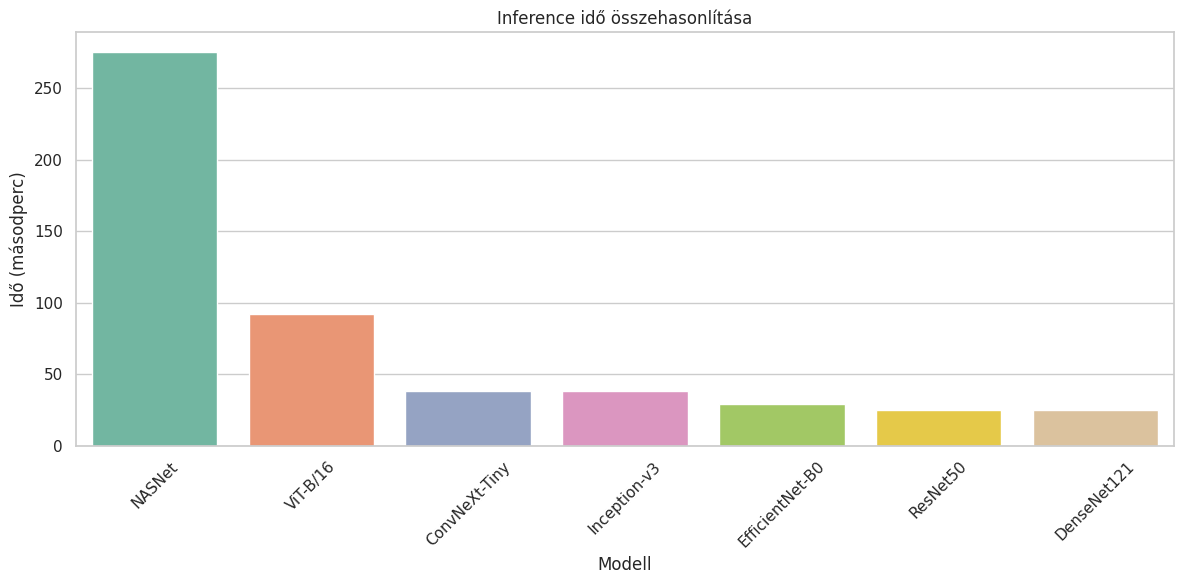
\includegraphics[width=0.75\textwidth]{images/phase01/summary03.png}
    \caption{sszehasonlító idő diagram a tanítás nélküli tesztekről.}
    \label{fig:timephase1}
    \end{figure}

    \begin{table}[H]
        \centering
        \caption{Tanítás nélküli modellek teljesítménye (Top-1 szerint csökkenő sorrendben)}
        \begin{tabular}{|l|c|c|c|c|c|c|}
        \hline
        \textbf{Modell} & \textbf{Top-1} & \textbf{Top-5} & \textbf{Prec.} & \textbf{Recall} & \textbf{F1} & \textbf{Idő (s)} \\
        \hline
        ViT-B/16 & 0.5308 & 0.8582 & 0.4629 & 0.4419 & 0.4307 & 92.13 \\
        ConvNeXt-Tiny & 0.5048 & 0.8471 & 0.4917 & 0.4369 & 0.4194 & 38.40 \\
        EfficientNet-B0 & 0.4802 & 0.8217 & 0.4137 & 0.4039 & 0.3829 & 28.89 \\
        Inception-v3 & 0.4763 & 0.8008 & 0.3833 & 0.3896 & 0.3683 & 38.06 \\
        ResNet50 & 0.4698 & 0.7962 & 0.3934 & 0.3797 & 0.3592 & 25.21 \\
        DenseNet121 & 0.4498 & 0.7806 & 0.3874 & 0.3611 & 0.3408 & 25.15 \\
        NASNet-A-Large & 0.2820 & 0.5408 & 0.3204 & 0.2799 & 0.2696 & 275.30 \\
        ResNet18 + Hybrid v2 & 0.0054 & 0.0379 & 0.0026 & 0.0063 & 0.0020 & 17.89 \\
        ResNet18 + Baseline & 0.0052 & 0.0304 & 0.0093 & 0.0072 & 0.0011 & 18.48 \\
        ResNet18 + Deep & 0.0050 & 0.0265 & 0.0003 & 0.0071 & 0.0006 & 15.54 \\
        ResNet18 + Hybrid v1 & 0.0047 & 0.0286 & 0.0041 & 0.0076 & 0.0014 & 15.54 \\
        \hline
        \end{tabular}
    \end{table}
    
    A vizsgálat során különféle előre betanított, tanítás nélküli (zero-shot) képklasszifikáló modellek teljesítményét értékeltem az SBPhotoThemes180k adathalmazon. A cél az volt, hogy felmérjem, mennyire képesek ezek a modellek az adathalmaz vizuális és tematikus sokszínűségének általános értelmezésére anélkül, hogy azokat kifejezetten ezen osztályokra tanítottuk volna.
    \\\\
    A Vision Transformer (ViT-B/16) érte el a legmagasabb Top-1 pontosságot (53,1\%) és F1-mutatót is (43,1\%), jelezve, hogy a nagy figyelmi mezővel dolgozó architektúra jól általánosít a komplex, valósághű témákon. Ezt szorosan követte a ConvNeXt-Tiny (F1: 41,9\%) és az EfficientNet-B0 (F1: 38,3\%), melyek hatékonyan egyensúlyozták a pontosságot és a számítási teljesítményt. A klasszikusabb modellek, mint ResNet50, DenseNet121 és Inception-v3, kissé alacsonyabb mutatókkal szerepeltek, de így is 35–38\% közötti F1-értéket produkáltak.
    \\\\
    A NASNet-A-Large különösen alacsony Top-1 pontosságot (28,2\%) mutatott, miközben számítási ideje kiugróan magas volt (275 s), ami gyenge hatékonyságra és a feladattal való inkompatibilitásra utal tanítás nélkül (tanítással nagyon hatékony). Ezzel szemben a saját fejlesztésű, ResNet18-alapú kísérleti modellek (Baseline, Hybrid, Deep variánsok) tanítás nélkül szinte semmilyen értelmezhető teljesítményt nem nyújtottak – F1-értékeik rendre 1\% alatt maradtak. Ez alátámasztja, hogy ezek a modellek jelenleg nem rendelkeznek megfelelő reprezentációs kapacitással, illetve nincs előzetes tudásuk az osztályozandó témákról.
    \\\\
    Összességében a tanítás nélküli tesztek alapján egyértelmű, hogy az erősebb, modern, pretrainelt architektúrák képesek hasznos predikciókat adni még finomhangolás nélkül is, míg a saját modellek kizárólag tanítással válhatnak versenyképessé.

\section{Következtetések az iteratív tanítás után kapott eredményekből.}

    \subsubsection{Összehasonlító Top-1 heatmap az iteratív tanításáról}
    \begin{figure}[H]
    \centering
    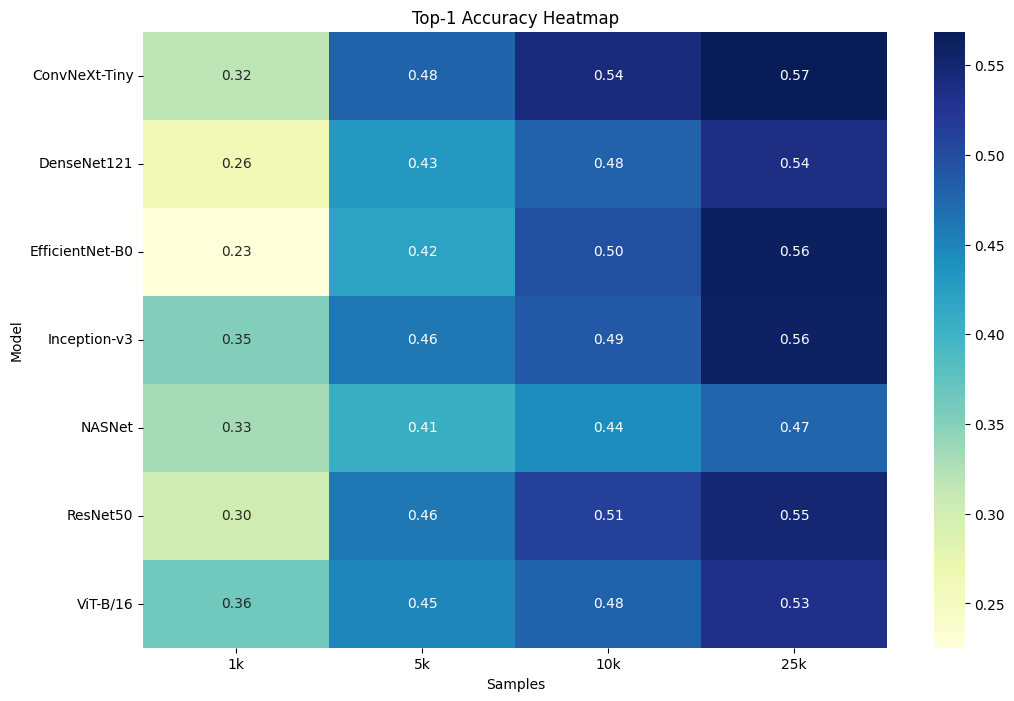
\includegraphics[width=0.8\textwidth]{images/phase03/top-1-heatmap.png}
    \caption{Összehasonlító Top-1 heatmap az iteratív tanításáról.}
    \label{fig:top1_heatmap}
    \end{figure}

    \subsubsection{Összehasonlító precision heatmap az iteratív tanításáról}
    \begin{figure}[H]
    \centering
    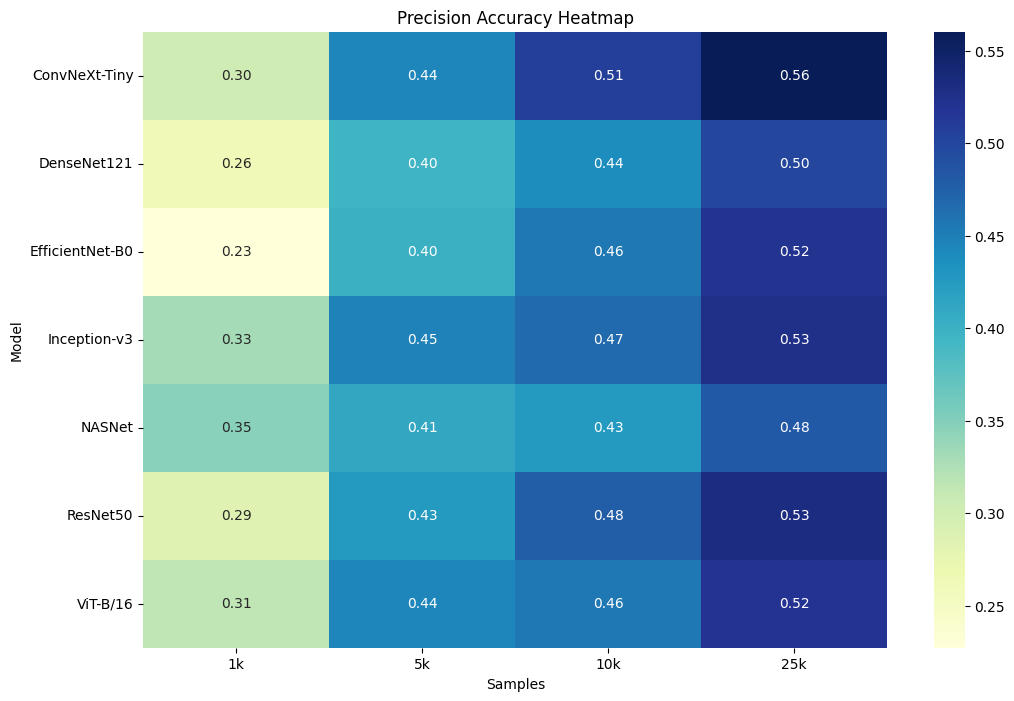
\includegraphics[width=0.8\textwidth]{images/phase03/precision_heatmap.png}
    \caption{Összehasonlító precision heatmap az iteratív tanításáról.}
    \label{fig:precision_heatmap}
    \end{figure}

    \begin{center}
        \begin{longtable}{llllllll}
        \caption{Összehasonlító táblázat az összes modell iteratív tanításáról.}\label{tab:phase4_summary_table}\\
        \toprule
        Modell & Minták & Top-1 & Top-5 & Precision & Recall & F1 & Time(s) \\
        \midrule
        \endfirsthead
        \toprule
        Modell & Minták & Top-1 & Top-5 & Precision & Recall & F1 & Time(s) \\
        \midrule
        \endhead
        ResNet50 & 1k & 0.302 & 0.650 & 0.285 & 0.315 & 0.282 & 31.490 \\
        ResNet50 & 5k & 0.460 & 0.777 & 0.425 & 0.476 & 0.432 & 31.720 \\
        ResNet50 & 10k & 0.513 & 0.818 & 0.478 & 0.542 & 0.490 & 31.710 \\
        ResNet50 & 25k & 0.550 & 0.838 & 0.531 & 0.598 & 0.544 & 31.820 \\
        DenseNet121 & 1k & 0.265 & 0.551 & 0.264 & 0.286 & 0.254 & 25.090 \\
        DenseNet121 & 5k & 0.431 & 0.751 & 0.396 & 0.449 & 0.405 & 24.870 \\
        DenseNet121 & 10k & 0.479 & 0.785 & 0.439 & 0.506 & 0.454 & 25.020 \\
        DenseNet121 & 25k & 0.537 & 0.821 & 0.500 & 0.574 & 0.517 & 24.710 \\
        EfficientNet-B0 & 1k & 0.225 & 0.477 & 0.227 & 0.249 & 0.218 & 24.750 \\
        EfficientNet-B0 & 5k & 0.421 & 0.750 & 0.401 & 0.463 & 0.412 & 24.640 \\
        EfficientNet-B0 & 10k & 0.498 & 0.806 & 0.455 & 0.526 & 0.473 & 24.670 \\
        EfficientNet-B0 & 25k & 0.563 & 0.846 & 0.521 & 0.607 & 0.546 & 24.780 \\
        ConvNeXt-Tiny & 1k & 0.317 & 0.623 & 0.303 & 0.345 & 0.303 & 25.450 \\
        ConvNeXt-Tiny & 5k & 0.478 & 0.794 & 0.444 & 0.490 & 0.452 & 25.450 \\
        ConvNeXt-Tiny & 10k & 0.542 & 0.827 & 0.508 & 0.566 & 0.514 & 25.270 \\
        ConvNeXt-Tiny & 25k & 0.569 & 0.849 & 0.560 & 0.623 & 0.568 & 25.330 \\
        ViT-B/16 & 1k & 0.364 & 0.665 & 0.314 & 0.353 & 0.314 & 41.850 \\
        ViT-B/16 & 5k & 0.448 & 0.733 & 0.444 & 0.480 & 0.436 & 41.930 \\
        ViT-B/16 & 10k & 0.478 & 0.764 & 0.456 & 0.507 & 0.454 & 41.930 \\
        ViT-B/16 & 25k & 0.533 & 0.819 & 0.519 & 0.591 & 0.531 & 42.080 \\
        Inception-v3 & 1k & 0.352 & 0.681 & 0.331 & 0.358 & 0.322 & 33.270 \\
        Inception-v3 & 5k & 0.460 & 0.787 & 0.447 & 0.486 & 0.447 & 33.300 \\
        Inception-v3 & 10k & 0.489 & 0.799 & 0.467 & 0.519 & 0.473 & 33.680 \\
        Inception-v3 & 25k & 0.560 & 0.844 & 0.525 & 0.582 & 0.534 & 33.460 \\
        NASNet & 1k & 0.332 & 0.613 & 0.346 & 0.369 & 0.326 & 81.040 \\
        NASNet & 5k & 0.406 & 0.691 & 0.410 & 0.428 & 0.384 & 81.540 \\
        NASNet & 10k & 0.444 & 0.766 & 0.425 & 0.474 & 0.413 & 81.460 \\
        NASNet & 25k & 0.475 & 0.806 & 0.481 & 0.529 & 0.469 & 81.430 \\
        \bottomrule
        \end{longtable}
    \end{center}
    \cleardoublepage
    
    A különböző képosztályozó modellek iteratív tanítása során egyértelműen kirajzolódik, hogy a mintaszám növelésével minden architektúra esetében fokozatos teljesítményjavulás tapasztalható. Ez jól mutatja a tanítási adathalmaz méretének meghatározó szerepét a hálózatok tanulóképességében és általánosító erejében.
    \\\\
    A ResNet50, mint klasszikus és stabil alapmodell, kiegyensúlyozott fejlődést mutatott: 1 000 mintával még csak 30,2\%-os Top-1 pontosságot ért el, míg 25 000 mintával ez az érték 54,9\%-ra nőtt. A DenseNet121 szintén hasonló mintázatot mutatott, bár teljesítménye némileg elmaradt a ResNet50-től. A NASNet, noha relatív jól szerepelt kis mintaszám mellett, a későbbi fázisokban lassabban fejlődött, és végül alacsonyabb F1-értékkel zárt, miközben a számítási ideje (81 s) lényegesen magasabb maradt.
    \\\\
    A ConvNeXt-Tiny és az EfficientNet-B0 modern architektúrák kiváló skálázódást mutattak: utóbbi különösen 25k mintával ért el kiemelkedő Top-1 pontosságot (56,3\%) és F1-mutatót (54,6\%), miközben megtartotta alacsony számítási igényét (~25 s). A ConvNeXt-Tiny 25k mintával a legjobb F1-értéket érte el (56,8\%), ami kiemelkedő arányosságot jelez a precizitás és a recall között. A ViT-B/16, bár Transformer-alapú modellként magasabb számítási igényt igényelt (~42 s), fokozatos és stabil növekedést mutatott, viszont nem ugrotta meg a legjobb CNN-ek pontosságát. A legkiegyensúlyozottabb teljesítményt az Inception-v3 nyújtotta, amely konzisztensen fejlődött, és 25k mintával 56\%-os Top-1 pontosságot ért el, F1-mutatója pedig elérte az 53,3\%-ot.
    \\\\
    Általánosságban elmondható, hogy minden modell profitált az iteratív tanításból, de a teljesítményük különböző sebességgel és hatékonysággal skálázódott. A modern, könnyű modellek (pl. EfficientNet-B0, ConvNeXt-Tiny) különösen hatékonynak bizonyultak kisebb számítási költség mellett is, míg a ViT és NASNet architektúrák több erőforrást igényeltek, de nem tudtak arányosan jobban teljesíteni. A mért F1-értékek jó képet adnak arról, mennyire tudtak a modellek kiegyensúlyozottan teljesíteni a helyes pozitív felismerések és a teljes visszakeresés aránya között.
    \\\\
    Ezek az eredmények megerősítik, hogy az adatmennyiség növelése kulcsfontosságú, ugyanakkor a modellválasztás – a számítási költségek és a pontosság fényében – szintén meghatározó tényező a gyakorlati alkalmazhatóság szempontjából.

\section{Következtetések a teljes tanítás után kapott eredményekből.}

    \begin{table}[H]
        \centering
        \caption{Teljes tanítás után elért eredmények (Top-1 szerint csökkenő sorrendben)}
        \begin{tabular}{|l|c|c|c|c|c|c|}
        \hline
        \textbf{Modell} & \textbf{Top-1} & \textbf{Top-5} & \textbf{Prec.} & \textbf{Recall} & \textbf{F1} & \textbf{Idő (s)} \\
        \hline
        EfficientNet-B0 & 0.7649 & 0.9421 & 0.7130 & 0.6950 & 0.7001 & 25.26 \\
        NASNet-A-Large & 0.7626 & 0.9470 & 0.7180 & 0.6875 & 0.6955 & 34.03 \\
        ConvNeXt-Tiny & 0.7624 & 0.9357 & 0.7168 & 0.6841 & 0.6947 & 25.67 \\
        ResNet50 & 0.7553 & 0.9351 & 0.7110 & 0.6808 & 0.6908 & 25.11 \\
        Inception-v3 & 0.7518 & 0.9320 & 0.6963 & 0.6787 & 0.6827 & 33.62 \\
        ViT-B/16 & 0.7414 & 0.9257 & 0.6935 & 0.6636 & 0.6730 & 42.40 \\
        DenseNet121 & 0.7400 & 0.9266 & 0.6811 & 0.6680 & 0.6696 & 25.23 \\
        ResNet18 + Baseline & 0.7303 & 0.9099 & 0.6777 & 0.6490 & 0.6568 & 18.54 \\
        ResNet18 + Hybrid v1 & 0.7276 & 0.9074 & 0.6828 & 0.6369 & 0.6536 & 16.13 \\
        ResNet18 + Deep & 0.7247 & 0.9000 & 0.6673 & 0.6336 & 0.6455 & 16.01 \\
        ResNet18 + Hybrid v2 & 0.7236 & 0.9011 & 0.6669 & 0.6391 & 0.6469 & 15.62 \\
        \hline
        \end{tabular}
    \end{table}

    \subsubsection{Teljes tanítás utáni összesítő Top-1 pontosság.}
    \begin{figure}[H]
    \centering
    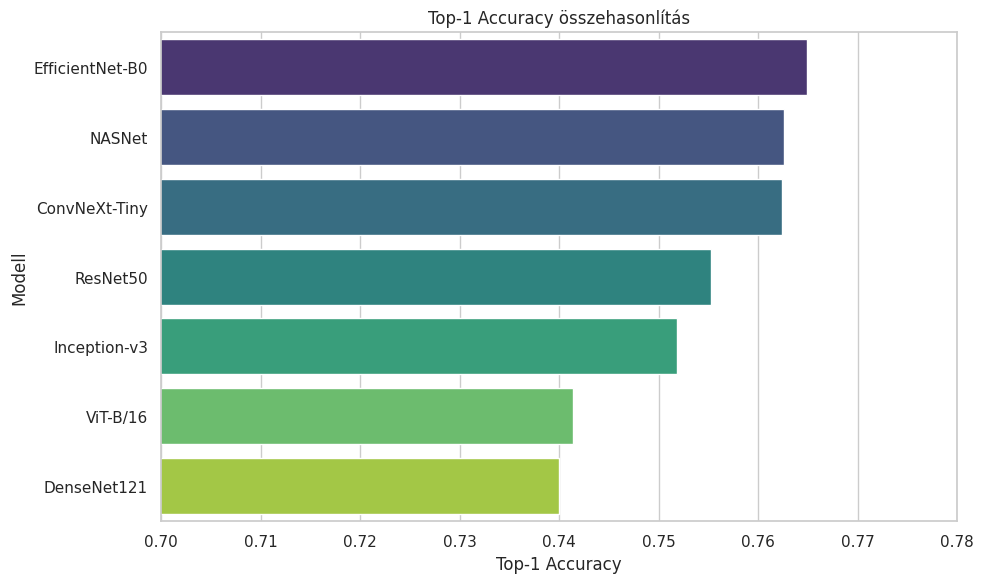
\includegraphics[width=0.7\textwidth]{images/phase02/phase02_summary_top1.png}
    \caption{Teljes tanítás utáni összesítő Top-1 pontosság.}
    \label{fig:phase02_01}
    \end{figure}

    \subsubsection{Teljes tanítás utáni összehasonlító Top-1 és Top-5 pontosság.}
    \begin{figure}[H]
    \centering
    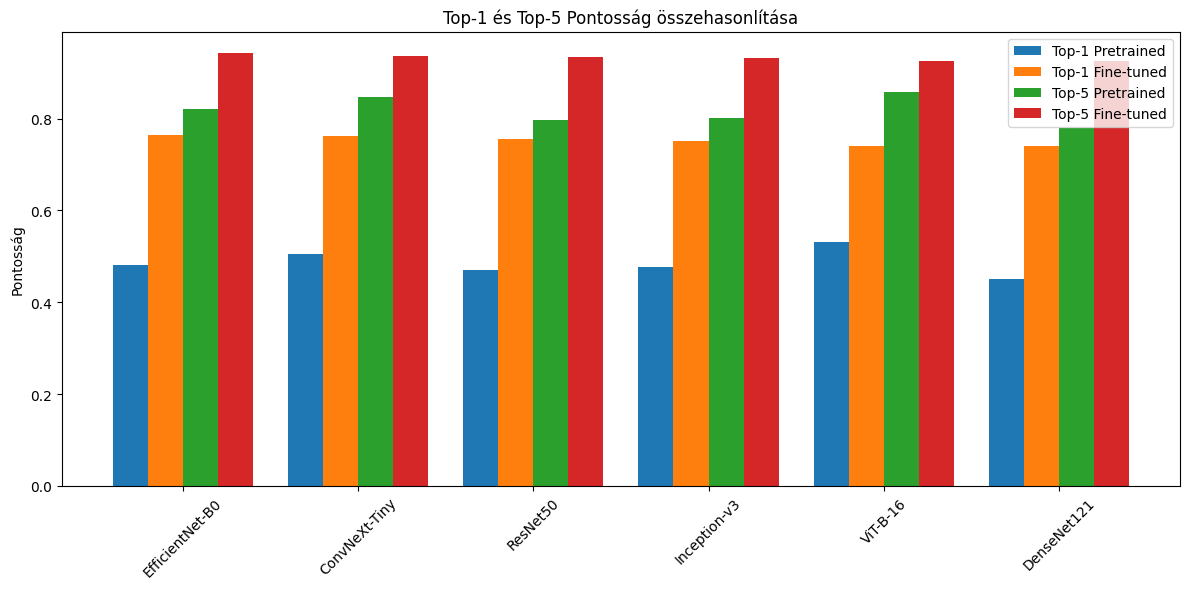
\includegraphics[width=0.7\textwidth]{images/phase02/phase02_summary_top1_vs_top5_pre_vs_fine.png}
    \caption{Teljes tanítás utáni összehasonlító Top-1 és Top-5 pontosság.}
    \label{fig:phase02_02}
    \end{figure}

    \subsubsection{Teljes tanítás utáni összesítő Top-1 pontosság.}
    \begin{figure}[H]
    \centering
    
\includegraphics[width=1.0\textwidth]{images/sum.png}
    \caption{Teljes tanítás utáni összesítő Top-1 pontosság.}
    \label{fig:phase02_03}
    \end{figure}

	A teljes tanítással végzett modellek elemzése alapján több fontos és meglepő megfigyelés is levonható:
	\\\\
    EfficientNet-B0 vezeti a mezőnyt: Bár eredetileg egy kompakt, mobilbarát hálózatként lett tervezve, az EfficientNet-B0 a legmagasabb Top-1 pontosságot (0.7649) és egyben az egyik legjobb F1-score értéket (0.7001) érte el. Ez kiemeli az architekturális hatékonyság és a méretezés szerepét a transfer learning során.
	\\\\
    NASNet-A-Large jelentős javulása: Tanítás nélkül a NASNet alulteljesített (0.2820 Top-1), de tanítással 0.7626 Top-1 pontosságot ért el. Ez azt mutatja, hogy bizonyos hálózatok „alvó potenciállal” rendelkeznek, és megfelelő finomhangolással rendkívül versenyképesek lehetnek.
	\\\\
    Transformer-alapú modellek stabilak, de nem verhetetlenek: A ViT-B/16 transformer modell jó teljesítményt mutatott (0.7414 Top-1), de nem emelkedett ki a többi CNN modell közül. Ez arra utal, hogy nagyobb adattömeg vagy hosszabb tanítási idő szükséges a transzformerek kiemelkedő teljesítményéhez a közepes méretű feladatokon.
	\\\\
    Könnyű fejekkel rendelkező ResNet18-alapú modellek is versenyképesek: A ResNet18 + különböző fejek kombinációja (Baseline, Deep, Hybrid v1/v2) 0.7236–0.7303 Top-1 pontosságot hozott. Ez figyelemre méltó, tekintve az alacsony számítási igényt és egyszerű architektúrát. A Baseline fej valamivel jobb eredményt produkált, mint a Deep vagy Hybrid fejek – valószínűleg az egyszerűbb modell kevésbé hajlamos az overfittingre a futási ideje viszont jelentősen jobb lett, így a Hybrid-v1 versenyképes eggyensúlyt tart a gyorsaság és a pontosság között és felveszi a versenyt a nagy modellekkel.
	\\\\
    Inference idő és teljesítmény kompromisszuma: A ViT és NASNet modellek jelentősen lassabbak (42–275 másodperc!), míg a ResNet18 alapú modellek gyorsak (15–18 másodperc). Ebből adódóan alkalmazás-specifikusan a legjobb választás nem mindig a legpontosabb modell – valós idejű rendszerekhez például egy ResNet18 + Hybrid fej lehet ideális kompromisszum.
	\\\\
    Top-5 pontosság is szoros versenyt mutat: A legtöbb modell 0.90 fölé emelkedett tanítás után, ami azt mutatja, hogy a modellek már nemcsak az első, hanem a legvalószínűbb néhány osztály közé is gyakran eltalálják a helyes címkét. Ez fontos többválaszos vagy javaslat-alapú rendszerek esetén.

\chapter{Összefoglaló}
\label{ch:summary}

A dolgozat célja a fotó osztályozási probléma vizsgálata volt neurális hálózatokkal saját nagyméretű címkézett adatbázison. 
A vizsgálat során összegyűjtöttem 180750 egyedi fotót az elmúlt 20 év saját készítésű képeiből, ebből címkézett adatbázist készítettem SBphotothemes180k néven kétféle címkézéssel.
Az ImageNet1K címkékből 114 kategória adta az első osztályozást a 300 képnél kisebb osztályok megszüntetése után, a Places365 címkékből 121 kategória adta a második osztályozást. Ezek után 80-10-10 arányban felosztottam tanító, validáló és tesztelő adathalmazra az adatbázist. Az adathalmaz képeit 224*244 méretű négyzetes jpg 80 tömörítésű képekké konvertáltam. Így a közel 2TB mennyiségű forrásképből nagyjából 10GB méretű adatbázis készült.
Az elkészült adatbázison vizsgáltam az osztályozási eloszlásokat, és az EXIF adatokat. Az osztályozások estén az átlagos osztályméret 1500 kép körül alakult, a medián 1000 kép körül alakult ami jó, de mivel természetes adatokról beszélünk, így az aszimmetria magas, 8.4 és a szórás is magas 3200 körüli tehát tipikus Long-tail eloszlást mutat.
Az EXIF adatok konverzió közbeni megőrzése és elemzése különösen fontos volt a részletes statisztikák elvégzéséhez és a későbbi vizsgálatok lehetőségeinek biztosításához. 
Az így elkészített adatbázis segítségével három fázisos vizsgálatot végeztem hét ismert és gyakran használt modellen. Ezek a modellek a ResNet50, DenseNet121, EfficientNet-B0, ConvNeXt-Tiny, ViT-B/16, Inception-v3, NASNet voltak. 
Az alkalmazott metrikák a következőek lettek: Top-1 és Top-5 pontosság, Precision, Recall, F1-score. Ezeken túl vizsgáltam a tanítás közbeni validációs és tanítási pontosságokat.
Mindhárom vizsgálatot ugyanazon az teszt adathalmazon végeztem, de más-más tanítóhalmazzal tanítottam. A három vizsgálati fázis a tanítás nélküli tesztelés, majd a teljes tanítás utáni vizsgálat volt, végül az iteratívan növekvő tanítóhalmaz vizsgálata következett. 
A vizsgálat első lépése a tanítás nélküli modellek tesztelése volt a beépített súlyokkal. Ekkor a modellek 50\% körüli Top 1 és 80\% körüli Top 5 pontosságot és 40\% körüli Precision-t nyújtottak. Itt a ConvNeXt-Tiny és ViT-B/16 emelkedtek ki.
A második fázis során a teljes 144000 képes tanítóhalmazon tanítottam minden modellt 10 epoch-on keresztül. Ekkor a modellek 75\% körüli Top 1 és 90\% körüli Top 5 pontosságot és 70\% körüli Precision-t nyújtottak a EfficientNet-B0 és NASNet emelkedtek ki.
Az utolsó vizsgálat során mindig a tanítatlan modellről indulva 1000, 5000, 10000, 25000 képes tanítóhalmazon vizsgáltam a modelleket szintén 10 epoch-on keresztül.
Az adataink alapján a ConvNeXt-Tiny és az EfficientNet-B0 modellek kiemelkedtek 25000 mintaszámmal történő tanítás után, míg a ResNet50 és DenseNet121 modellek gyengébben teljesítettek az alacsonyabb mintaszámokon, de növekvő mintaszámmal jelentős javulást mutattak. Eközben az Inception-v3 és a ViT-B/16 pedig a kis adathalmazon mutatott pontosság terén emelkedtek ki.
Ezután megkíséreltem elkészíteni egy kis méretű, lokális alkalmazásra optimalizált erőforrástakarékos modellt a ResNet18-ra építve egy saját fejrész kifejlesztésével. 
Ennek során 4 modellt készítettem, egy egyrétegű, egy mély, és két modern fejrésszel rendelkezőt. Ezen a négy modellen is elvégeztem a fent ismertetett három mérési fázist. Az egyrétegű fej meglepően jól teljesített, a mély fejrész viszont jelentősen alulmaradt a fenti metrikákban, a modern fejrész csak kicsit nyújtott nagyobb pontosságot, mint az egyrétegű, de jelentősen gyorsabban futott. Összességében a kifejlesztett modell csak kis mértékben maradt alul a vizsgált hatalmas modellektől, de futási teljesítménye sokkal jobb azokénál így nem pontosságkritikus, de erőforráskímélő megoldásokhoz, például hordozható eszközök számára ideális.
Összességében a nagyméretű adathalmaz, a többféle osztályozás, a nagy mennyiségű mért adat és a saját modellek további vizsgálatok alapját képezhetik a jövőben.

\chapter{ További lehetőségek}
A dolgozat során számos lépést sikerült megvalósítani, azonban több irány is kínálkozik a munka továbbfejlesztésére. Az SBPhotoThemes180k adatbázis Places365 szerinti osztályozásának részletes vizsgálata eddig nem történt meg, pedig ez értékes kiegészítő információkat nyújthatna az adathalmaz tematikus és vizuális jellemzőiről, valamint új szempontokat nyithatna a modellalkalmazásban.

Emellett a dolgozatban bemutatott Hybrid-v2 modell is további fejlesztési lehetőségeket rejt magában. A hálózati architektúra finomhangolása, további adataugmentációs eljárások integrálása vagy alternatív veszteségfüggvények alkalmazása mind hozzájárulhatnának a modell robusztusságának és általánosítási képességének javításához.

A jövőben ezen irányok célzott vizsgálata és továbbfejlesztése lehetőséget nyújthat nemcsak a meglévő eredmények elmélyítésére, hanem új, alkalmazásorientált megközelítések kidolgozására is a képosztályozás területén.

\chapter{ Befejezés}
A dolgozat során valós fotókból kiindulva egy egyedi képadatbázist állítottam össze, amelyet részletesen elemeztem. A munkához saját szoftveres eszközkészletet fejlesztettem, amelynek segítségével meglévő konvolúciós neurális hálózatokat teszteltem, majd az így szerzett tapasztalatokra építve saját modellt terveztem és optimalizáltam.

A diplomamunka elkészítése során lehetőségem nyílt arra, hogy elméleti ismereteimet gyakorlati tapasztalatokkal mélyítsem el egy összetett, több lépésből álló feladaton keresztül. A képfeldolgozás, az adatbázis-építés és a neurális hálózatokkal való munka során nemcsak technikai tudásom fejlődött, hanem rendszerszemléletem, problémamegoldó készségeim és az önálló munkavégzéshez szükséges attitűdöm is formálódott.

Ez a projekt számomra különleges jelentőséggel bírt, mivel lehetőséget adott arra, hogy összekapcsoljam a fotózás iránti szenvedélyemet a tanulmányaimmal, a mesterséges intelligencia iránti szakmai érdeklődésemmel éa a vizualitásaL \\
Örömmel és büszkeséggel tekintek vissza erre az útra, amely nemcsak szakmailag gazdagított, hanem személyesen is sokat nyújtott. Örülök, hogy végigcsinálhattam.

\cleardoublepage

% Main content END--------------------------------------------------

% Bibliography (mandatory)
\phantomsection
\addcontentsline{toc}{chapter}{\biblabel}
\printbibliography[title=\biblabel]
\cleardoublepage

% List of figures (optional) - useful over 3-5 figures
\phantomsection
\addcontentsline{toc}{chapter}{\lstfigurelabel}
\listoffigures
\cleardoublepage

% List of tables (optional) - useful over 3-5 tables
\phantomsection
\addcontentsline{toc}{chapter}{\lsttablelabel}
\listoftables
\cleardoublepage

% List of codes (optional) - useful over 3-5 code samples
\phantomsection
\addcontentsline{toc}{chapter}{\lstcodelabel}
\lstlistoflistings
\cleardoublepage

\appendix

% --- Melléklet A kezdete ---
%\chapter*{Melléklet A: Mérési napló}
%\addcontentsline{toc}{chapter}{Melléklet A: Mérési napló}
%
\includepdf[pages=-]{measurement_log.pdf}

%\chapter*{Melléklet B: Az elkészített szoftverek}
%\addcontentsline{toc}{chapter}{Melléklet B: Az elkészített szoftverek}
%
\includepdf[pages=-]{software_log.pdf}

\end{document}
